%%
%% $Id$
%%
%% Document: Hauptdokument des `makeindex4'-Projektes
%%

%%
%% $Id$
%%
%% Document:
%%


%%\documentclass[11pt]{article}
\documentclass[11pt]{report}

\usepackage{oldgerm}
\usepackage{a4}
\usepackage{xspace}
\usepackage{afterpage}
\usepackage{theorem}
\usepackage{fancyheadings}
\usepackage{ifthen}
%%\usepackage{shortvrb}
\usepackage[hang,bf,small]{caption}

%\usepackage{multicol}

\usepackage{epsfig}

% its absolutely necessary to include german AFTER epsfig
\usepackage{german}
\usepackage[isolatin]{inputenc}


%% These are my styles

%% Need to set \ReportMode=1 because of the incompatibilities with
%% foil.cls. See stdwrk.sty for further details.

\newcommand{\ReportMode}{1}
\usepackage{stdwrk}

\usepackage{xindy}
\usepackage{figsect}
\usepackage{environments}
\usepackage[help,level4]{tableofcontents}
\usepackage[help,ParagraphLikeSections]{sectioning}
\usepackage{footnotelist}


%%%%% Here comes stuff from Guy Steele..

%%\makeatletter
%%% The \null in the following is intended to suppress hyphenation
%%% in code words not already containing hyphens.  The \leavevmode
%%% is needed to prevent vertical mode from swallowing the \null.
%%%%%\def\cd#1{\leavevmode{\cf \null#1}}
%%\def\cd{\leavevmode\begingroup\cf\@cd}
%%\def\@cd#1{\null#1\endgroup}
%%\def\cf{\ttfamily\frenchspacing}
%%\makeatother

%%%%% stuff from Guy Steele ends here.


%\makeindex

%%
%% $Id$
%%
%% Document: Praeambel mit Definitionen
%%

\hyphenation{%
  Lo-ka-tions-re-fe-renz
  Lo-ka-tions-re-fe-ren-zen
  In-de-xes In-de-xen
  Do-ku-ment-alpha-bet
  Do-ku-ment-alpha-bets
  Do-ku-ment-alpha-be-tes
  Sor-tier-alpha-bet
  Sor-tier-alpha-bets
  Sor-tier-alpha-bet-es
  Sor-tier-ungs-alpha-bet
  Sor-tier-ungs-alpha-bets
  Sor-tier-ungs-alpha-be-tes
  Kon-fi-gu-ra-tion
  Ba-sis-alpha-bet
  Ba-sis-alpha-bets
  Ba-sis-alpha-be-tes
  Sym-bol-alpha-bet
  Sym-bol-alpha-bets
  Sym-bol-alpha-be-tes
  Ka-te-go-rie-attri-but
  Ka-te-go-rie-attri-buts
}

%% Local Variables:
%% mode: latex
%% TeX-master: "makeindex4.tex"
%% End:

%%
%% $Log$
%% Revision 1.3  1995/11/03 15:53:17  kehr
%% Neuformulierung der join-range()-Funktion.
%%
%% Revision 1.2  1995/10/20  11:57:33  kehr
%% Korrektur nach Klaus' Durchsicht.
%%
%% Revision 1.1  1995/10/16  17:31:52  kehr
%% Initial checkin of Report and Presentation.
%%
%% Revision 1.21  1995/10/06  23:05:18  kehr
%% Korrektur nach der Durchsicht von Karin.
%%
%% Revision 1.20  1995/09/22  01:12:08  kehr
%% Zweite �berarbeitung nch der inhaltlichen Korrektur. Au�erdem habe
%% ich das Logo zu MacIndex ver�ndert. Hat jetzt mehr pepp !
%%
%% Revision 1.19  1995/09/21  00:05:48  kehr
%% Erste Ver�nderungen nach der inhaltlichen Korrektur durch Joachim am
%% 20.Sep.95. Fast alle Dateien d'sind davon betroffen. Au�erdem sind noch zwei
%% neue Abbildungen hinzugekommen.
%%
%% Revision 1.18  1995/09/06  18:52:52  kehr
%% Made final changes before giving for correction.
%%
%% Revision 1.17  1995/08/28  18:08:19  kehr
%% Neue Einspielung der xfig-Dateien
%%
%% Revision 1.16  1995/07/04  09:46:31  kehr
%% Weitere �nderungen. Bin aber fast fertig.
%%
%% Revision 1.15  1995/07/04  00:46:54  kehr
%% Bald ist's soweit ;-)
%% Ich habe heute die generelle Umstrukturierung vorgenommen und einige
%% Teile herausgeschmissen. Die Indexverarbeitung mu� noch �berarbeitet werden.
%%
%% Revision 1.14  1995/06/18  23:32:25  kehr
%% Schlu� f�r heute. Genug geschafft.
%%
%% Revision 1.13  1995/06/17  20:36:31  kehr
%% Habe die Lokationsreferenzverarbeitung umstrukturiert und besser
%% definiert. DIe Buchstabengruppen m�ssen noch beendet werden und der
%% Algorithmus zum Mischen und Sortieren der Lokationsreferenzen mu�
%% fertiggestellt werden.
%%
%% Revision 1.12  1995/06/13  21:55:17  kehr
%% Habe heute die Formulierung des Algorithmus controlled-jojo-traverse
%% fertiggestellt. Desweiteren Fehler in der Anwendung der \lindent-Umgebung
%% gefunden. Ich mu� noch die Matrix f�r die Definition der Ausgabekommandos
%% und der Angabe im Indexstyle entwickeln.
%%
%% Revision 1.11  1995/06/09  20:59:52  kehr
%% Superviel gemacht heute ;-)
%%
%% Revision 1.10  1995/06/08  20:19:48  kehr
%% Bibliographie erweitert.
%%
%% Revision 1.9  1995/06/06  23:50:15  kehr
%% Modellentwurf weitergebracht.
%%
%% Revision 1.8  1995/06/06  11:50:36  kehr
%% Weitere Bearbeitung des Modellentwurfs.
%%
%% Revision 1.7  1995/05/31  16:14:59  kehr
%% Dokumant- und Sortierungsalphabet entwickelt. Makefile�nderungen und
%% Stylever�nderungen.
%%
%% Revision 1.6  1995/05/28  21:37:12  kehr
%% Neue �berarbeitete Version.
%% Inhaltliche �nderungen:
%%   Glossar hinzugenommen. Einleitung mit Datenflu�graph. Kleinere
%%   �nderungen an der Beschreibung des International Makeindex.
%% System�nderungen:
%%   Makefile-�nderungen, Stil�nderungen, Titelseite
%%
%% Revision 1.5  1995/05/05  23:07:15  kehr
%% Ge�nderte Datenstrukturen mit enumerate und neuen labels f�r enumerate
%%
%% Revision 1.4  1995/05/05  22:25:06  kehr
%% Ge�nderte Struktur mit einleitung.tex
%% Zwischenspeicherung vor der Umstellung der Definitionen
%%
%% Revision 1.3  1995/04/30  16:14:11  kehr
%% Trennung in Einleitung, Einf�hrung und Analyse. Evtl. sollten die Filenamen
%% entsprechend anepa�t werden. Dar�berhinaus Analyse weitergef�hrt.
%%
%% Revision 1.2  1995/04/25  01:09:40  kehr
%% Analyse und Modellentwurf weitergebracht.
%%
%% Revision 1.1  1995/04/22  21:05:41  kehr
%% Erstes Setup der Studienarbeit des Makeindex4-Projektes
%%

%%% Local Variables:
%%% mode: plain-tex
%%% TeX-master: t
%%% End:

\input{words.tex}

\tolerance=1000
\emergencystretch=20pt
%\parskip=6pt

\overfullrule 2mm

%
% aktivieren der fancyheadings
%
\pagestyle{fancy}
\newcommand{\titleshape}[1]{\textbf{#1}}
%
% falls die Headings �ber die Marginalien hinausragen sollen
%
%\addtolength{\headwidth}{\marginparsep}
%\addtolength{\headwidth}{\marginparwidth}
%
% Korrektur um overfull vbox zu unterbinden
%
\addtolength{\headheight}{2pt}
%
% section und subsection im Kopf redefinieren
%
\renewcommand{\chaptermark}[1]{\markright{\textbf{\thechapter}\ %
      \titleshape{#1}}}
\renewcommand{\sectionmark}[1]{\markright{\textbf{\thesection}\ %
      \titleshape{#1}}}
%
% linken und rechten Kopf definieren
%
\lhead{\fancyplain{}{\let\uppercase\relax\bfseries\rightmark}}
\rhead{\fancyplain{}{\bfseries\thepage}}
\cfoot{}

%% Aktivieren des Pipe-Zeichens als Abbrev f�r \verb|...|
%% Dies mu� an den gew�nschten Stellen im Text geschehen, da eine
%% globale Definiton nicht m�glich ist.
%\MakeShortVerb{\|}
%\DeleteShortVerb{\|}

\overfullrule 1mm

\begin{document}

%% Local Variables:
%% mode: latex
%% TeX-master: "makeindex4.tex"
%% End:

%%
%% $Log$
%% Revision 1.1  1995/10/16 17:31:56  kehr
%% Initial checkin of Report and Presentation.
%%
%% Revision 1.15  1995/10/06  23:05:18  kehr
%% Korrektur nach der Durchsicht von Karin.
%%
%% Revision 1.14  1995/09/22  01:12:09  kehr
%% Zweite �berarbeitung nch der inhaltlichen Korrektur. Au�erdem habe
%% ich das Logo zu MacIndex ver�ndert. Hat jetzt mehr pepp !
%%
%% Revision 1.13  1995/09/21  00:05:48  kehr
%% Erste Ver�nderungen nach der inhaltlichen Korrektur durch Joachim am
%% 20.Sep.95. Fast alle Dateien d'sind davon betroffen. Au�erdem sind noch zwei
%% neue Abbildungen hinzugekommen.
%%
%% Revision 1.12  1995/09/06  18:52:53  kehr
%% Made final changes before giving for correction.
%%
%% Revision 1.11  1995/07/04  00:46:55  kehr
%% Bald ist's soweit ;-)
%% Ich habe heute die generelle Umstrukturierung vorgenommen und einige
%% Teile herausgeschmissen. Die Indexverarbeitung mu� noch �berarbeitet werden.
%%
%% Revision 1.10  1995/06/17  20:36:31  kehr
%% Habe die Lokationsreferenzverarbeitung umstrukturiert und besser
%% definiert. DIe Buchstabengruppen m�ssen noch beendet werden und der
%% Algorithmus zum Mischen und Sortieren der Lokationsreferenzen mu�
%% fertiggestellt werden.
%%
%% Revision 1.9  1995/06/09  20:59:53  kehr
%% Superviel gemacht heute ;-)
%%
%% Revision 1.8  1995/06/08  00:35:55  kehr
%% Was soll ich blo� schreiben ???
%%
%% Revision 1.7  1995/06/07  20:59:14  kehr
%% Und weiter am Modellentwurf. Spezifikation des Indexstyles vorerst
%% fertig. Es fehlt noch die Eingabegrammatik.
%%
%% Revision 1.6  1995/06/06  17:51:03  kehr
%% Commit um die �nderungen festzuhalten.
%%
%% Revision 1.5  1995/05/29  00:22:44  kehr
%% Die Einleitung ist somweit fertig und die Analyse mu� jetzt noch
%% beendet werden. Mir fehlt da noch eine vern�nftige Idde f�r die
%% Alphabete und deren Definitionen.
%%
%% Revision 1.4  1995/05/28  21:37:12  kehr
%% Neue �berarbeitete Version.
%% Inhaltliche �nderungen:
%%   Glossar hinzugenommen. Einleitung mit Datenflu�graph. Kleinere
%%   �nderungen an der Beschreibung des International Makeindex.
%% System�nderungen:
%%   Makefile-�nderungen, Stil�nderungen, Titelseite
%%
%% Revision 1.3  1995/05/05  22:25:06  kehr
%% Ge�nderte Struktur mit einleitung.tex
%% Zwischenspeicherung vor der Umstellung der Definitionen
%%
%% Revision 1.2  1995/04/25  01:09:41  kehr
%% Analyse und Modellentwurf weitergebracht.
%%
%% Revision 1.1  1995/04/22  21:05:41  kehr
%% Erstes Setup der Studienarbeit des Makeindex4-Projektes
%%


%%
%% $Id$
%%
%% Document: Titelseite
%%

\begin{titlepage}

\vspace*{\stretch{1}}

%\HRule

\vspace*{2mm}

\begin{center}

\MKXVIER

\vspace*{2.5mm}

\rule{9cm}{0.7pt}

\vspace*{5mm}

{\Large\textrm{Ein Flexibles Indexierungssystem}}

\vspace*{2mm}

\vspace*{\stretch{0.7}}

\large
Studienarbeit
\\[2mm]
{\scshape Roger Kehr}
\\[2mm]
November 1995

\vspace*{\stretch{0.3}}

% kludge to get athene-logo printed (displays wrong)
\font\athenefont=athenes scaled 800
\def\athene{{\athenefont\char0}}
{\athene}

\vspace*{\stretch{0.3}}
Institut f�r Theoretische Informatik
\\[2mm]
FG Systemprogrammierung
\\[2mm]
Technische Hochschule Darmstadt
\end{center}

\vspace*{\stretch{0.5}}

\end{titlepage}

%% Local Variables:
%% mode: latex
%% TeX-master: "makeindex4.tex"
%% End:

%%
%% $Log$
%% Revision 1.5  1995/11/20 17:57:02  kehr
%% Allerletzte �nderungen.
%%
%% Revision 1.4  1995/11/14  16:05:59  kehr
%% Made two more corrections on the report.
%%
%% Revision 1.3  1995/11/08  16:17:11  kehr
%% New correction.
%%
%% Revision 1.2  1995/10/26  16:05:37  kehr
%% Ver"anderung des Titels und Hinzunahme des Abstracts und der Danksagung.
%%
%% Revision 1.1  1995/10/16  17:31:57  kehr
%% Initial checkin of Report and Presentation.
%%
%% Revision 1.11  1995/10/06  23:05:19  kehr
%% Korrektur nach der Durchsicht von Karin.
%%
%% Revision 1.10  1995/09/22  01:12:09  kehr
%% Zweite �berarbeitung nch der inhaltlichen Korrektur. Au�erdem habe
%% ich das Logo zu MacIndex ver�ndert. Hat jetzt mehr pepp !
%%
%% Revision 1.9  1995/09/21  00:05:49  kehr
%% Erste Ver�nderungen nach der inhaltlichen Korrektur durch Joachim am
%% 20.Sep.95. Fast alle Dateien d'sind davon betroffen. Au�erdem sind noch zwei
%% neue Abbildungen hinzugekommen.
%%
%% Revision 1.8  1995/08/28  18:08:19  kehr
%% Neue Einspielung der xfig-Dateien
%%
%% Revision 1.7  1995/07/04  00:46:56  kehr
%% Bald ist's soweit ;-)
%% Ich habe heute die generelle Umstrukturierung vorgenommen und einige
%% Teile herausgeschmissen. Die Indexverarbeitung mu� noch �berarbeitet werden.
%%
%% Revision 1.6  1995/06/13  21:55:18  kehr
%% Habe heute die Formulierung des Algorithmus controlled-jojo-traverse
%% fertiggestellt. Desweiteren Fehler in der Anwendung der \lindent-Umgebung
%% gefunden. Ich mu� noch die Matrix f�r die Definition der Ausgabekommandos
%% und der Angabe im Indexstyle entwickeln.
%%
%% Revision 1.5  1995/05/31  19:18:54  kehr
%% Fertigstellung des Analyse-Abschnitts (Hoffentlich ;-).
%%
%% Revision 1.4  1995/05/28  21:37:13  kehr
%% Neue �berarbeitete Version.
%% Inhaltliche �nderungen:
%%   Glossar hinzugenommen. Einleitung mit Datenflu�graph. Kleinere
%%   �nderungen an der Beschreibung des International Makeindex.
%% System�nderungen:
%%   Makefile-�nderungen, Stil�nderungen, Titelseite
%%
%% Revision 1.3  1995/04/30  16:14:12  kehr
%% Trennung in Einleitung, Einf�hrung und Analyse. Evtl. sollten die Filenamen
%% entsprechend anepa�t werden. Dar�berhinaus Analyse weitergef�hrt.
%%
%% Revision 1.2  1995/04/25  01:09:41  kehr
%% Analyse und Modellentwurf weitergebracht.
%%
%%

\newpage

\pagenumbering{roman}

\tableofcontents

\newpage
\listoffigures
\listoftables

%% %%
%% $Id$
%%
%% Document: Abstract
%%

\begin{abstract}

  \noindent Dieser Bericht beschreibt die Ergebnisse einer
  Studienarbeit, die 1995 am Institut f"ur Theoretische Informatik an
  der Technischen Hochschule Darmstadt erstellt wurde. Ziel des
  Projektes war eine theoretische Analyse der Anforderungen an
  Indexierungssysteme und eine prototypische Implementierung.

  Indexierungssysteme verarbeiten die von einem Textsatzsystem
  erzeugten Indexierungsinformationen, um daraus einen sortierten und
  mit Ausgabeinformationen versehenen Index zu generieren. Dieser wird
  in der Regel dann wieder dem Textsatzsystem zugef"uhrt. Gegenstand
  der Studienarbeit war eine Analyse der Leistungsf�higkeit
  bestehender Systeme und eine darauf aufbauende Entwicklung eines
  theoretischen Gesamtmodells der Indexverarbeitung. Besonderen Wert
  wurde dabei auf die Verarbeitung von Lokationsreferenzen und die
  Ausgabeformatierung gelegt. Hohe Benutzerkonfigurierbarkeit und
  Flexibilit"at waren weitere Ziele bei der Entwicklung. Eine
  Teilimplementierung der Kernaspekte des Modells wurde vorgenommen,
  um die wesentlichen Aspekte zu "uberpr"ufen.


\end{abstract}


%%% Local Variables:
%%% mode: latex
%%% TeX-master: t
%%% End:


\newpage
\pagenumbering{arabic}

%%
%% $Id$
%%
%% Document: Einleitung f�r das `makeindex4' - Projekt
%%

\chapter{Vorwort}

\remark{Index als Bestandteil von Literatur}%
Die Qualit�t von guten Lehr- und Sachb�chern ist in erster Linie eine
Frage der methodischen und didaktischen Vermittlung von Wissen.
Weiterhin kann man auf die Funktion eines Buches als Nachschlagewerk
besonderen Wert legen. Es sollte m�glich sein, durch Nachschlagen nach
Stichw�rtern und Begrif"|fen schnell an gew�nschte Informationen zu
gelangen. Lehrb�cher sind in der Regel ohne einen gut stukturierten
Index nicht als Nachschlagewerk verwendbar.
%% Oft genug hat man den Eindruck, als ob die Autoren den Leser nach dem Motto
%% \flqq\textit{Suchet, so werdet ihr finden.}\frqq{} arbeiten lassen.
Viele Lehrb�cher weisen leider einen sehr unvollst�ndigen Index auf,
in welchem wichtige Begrif"|fe fehlen oder die Verweise auf die
entsprechenden Seiten im Buch fehlerhaft oder ungen�gend sind. Sie
enthalten dadurch ein schlecht strukturiertes und un�bersichtliches
Stichwortverzeichnis und verlieren dadurch entscheidend an Qualit�t.

\remark{M�ngel bestehender Systeme}%
Grund f�r diese M�ngel sind oft nicht ausreichende Systeme zur
Erstellung solcher Indexe. Ist es bei maschinell lesbaren Texten
meistens m�glich, durch entsprechende Suche nach bestimmten
Begrif"|fen ansatzweise trotzdem an die gew�nschten Textstellen zu
gelangen, ist dies prinzipiell bei gedruckter Literatur nicht m�glich,
und der Leser ist grunds�tzlich immer auf das Stichwortverzeichnis
angewiesen.

\remark{Besondere Bed�rfnisse}%
Weiterhin trifft man insbesondere in den Naturwissenschaften immer
h�ufiger auf spezielle W�nsche der Autoren. Zu diesen W�nschen z�hlen
Indexe mit mehrsprachigen Eintr�gen, die Verwendung verschiedenartiger
Indexverweise auf Seitenummern, Gliederungsebenen, Anh�nge, Symbole
\etc, welche mit herk�mmlichen Indexierungssystemen nicht
zufriedenstellend erf�llt werden k�nnen. Prinzipiell sollte ein
Indexierungsprogramm auch in der Lage sein, spezielle
In\-dex\-in\-for\-ma\-tion\-en wie HyperText-Links o.�.\ zu verwalten.
Viele der existierenden Systeme sind in einzelnen Details sehr
leistungsf�hig, aber ein �bergreifendes Konzept fehlt meist und sie
sind deshalb nur begrenzt einsetzbar. Beispiele f�r solche Systeme
sind das \Makeindex-System~\cite{Chen:SPE-19-9-897} in Verbindung mit
dem \TeX{}- \cite{texbook} \bzw{} \LaTeX-System~\cite{latex} oder
moderne interaktive Textverarbeitungssysteme wie {\slshape
  StarWriter\/}~\cite{starwriter} oder {\slshape
  Word\,f�r\,Windows\/}~\cite{winword}.

Die grunds�tzliche Problematik, welche Begrif"|fe und Stichw�rter in
einen Index aufzunehmen sind, auf welche Stellen im Text verwiesen
werden soll, wie Referenzen optisch unterschiedlich hervorzuheben sind
\usw, ist nicht Gegenstand dieser Arbeit. Diese Aufgabe wird
�blicherweise vom Autor eines Buches �bernommen, denn sie erfordert
Kenntnis von den Inhalten und der Struktur des Textes und soll auch
auf Schwerpunkte innerhalb des Buches hinweisen. Weitere Betrachtungen
zu diesem Themenaspekt finden sich in \cite{Lamb:EPODD-6-1-23} und
\cite{chicago}.

%\remark{Text-Tagging}%
%Wir betrachten hier diese als \emph{Text-Tagging} bezeichnete Aufgabe
%als bereits gel�st und erwarten als Eingabedaten f�r unser Modell
%einen irgendwie strukturierten Datenstrom von einzelnen ungeordneten
%Indexeintr�gen, die von dem zu entwerfenden System aufbereitet,
%gemischt und sortiert werden, und anschlie�end zu einem fertigen Index
%zusammengef�gt werden.

\remark{Gegenstand der Studienarbeit}%
Gegenstand der Arbeit ist eine grunds�tzliche Analyse der
Erfordernisse an ein Indexierungssystem und die Entwicklung eines
m�glichst universellen Modells der Indexverarbeitung. Dieses Modell
soll den \oa Anspr�chen in m�glichst vielen Bereichen gerecht werden.
Neue erweiterte Mechanismen zur Generierung eines Indexes werden
vorgestellt und entsprechende Algorithmen eingef�hrt.

Basierend auf diesem Modell wird dann eine Implementierung der
grundlegenden Verfahren des Modells vorgenommen, um die
grunds�tzlichen Mechanismen in der Praxis zu verifizieren.


\chapter{Einf�hrung}
\label{sec:ana:Einfuehrung}

Wir werden in dem nun folgenden Abschnitt die grunds�tzliche Funktion
eines Indexierungssystems und seine Einbettung in den Textsatzproze�
darlegen.  In Abschnitt~\ref{sec:analyse} werden wir eine vertiefte
Analyse bestehender Systeme durchf�hren. Eigene Erkenntnisse werden
dargelegt und insbesondere die Lokationsreferenzen werden als
Schwerpunkt dieser Arbeit in
Abschnitt~\ref{sec:ana:Lokationsreferenzen} vertieft untersucht. In
Abschnitt~\ref{sec:modellentwurf} werden wir die aus der Analyse
gewonnenen Informationen in ein Modell der Indexverarbeitung abbilden.
Es folgt ein �berblick �ber die Verarbeitungsvorg�nge innerhalb des
Modells in Abschnitt~\ref{sec:indexverarbeitung}. In
Abschnitt~\ref{sec:implementierung} finden sich Informationen �ber die
erfolgte Implementierung des Systems. Den Abschlu� bilden die
Zusammenfassung in Abschnitt~\ref{sec:zusammenfassung} und ein Glossar
in Abschnitt~\ref{sec:glossar}.


\section*{Datenflu� in einem Indexierungssystem}

Der Datenflu�, an welchem ein Indexierungssystem beteiligt ist, ist in
Abbildung~\ref{fig:datenfluss} dargestellt. Das Textsatzsystem liefert
die Rohdaten der Indexeintr�ge in einem festgelegten Format. Das
Indexsystem liest zun�chst s�mtliche f�r den Verarbeitungsproze�
ben�tigten Informationen aus der Indexstyle-Datei\remark{Indexstyle}
ein. Anschlie�end werden die Rohdaten des Indexes eingelesen. Die
Indexeintr�ge werden daraufhin gemischt und sortiert. Dieser Proze"s
besteht aus der Verarbeitung der Stichw"orter und den dazugeh"origen
Verweisen auf das Dokument. Diese Verweise werden mit
\emph{Lokationsreferenz} bezeichnet. Die entsprechenden Misch- und
Sortierregeln sind im Indexstyle angegeben. Zuletzt wird der komplette
Index mit einem Markup versehen und dem Textsatzsystem zur
Weiterverarbeitung zugef�hrt.

Besondere Wichtigkeit liegt dabei auf der benutzerdefinierbaren
Konfiguration \remark{Benutzer\-definierbare Konfiguration}des
Indexstyles. M�glichst viele Parameter des Systems sollten von
Benutzer einstellbar sein, um eine m�glichst hohe Anpassungsf�higkeit
zu gew�hrleisten.

Wie man aus diesem Konzept erkennen kann, ist unser System eine Art
\emph{Indexprozessor}. Ein Index wird in einem kompletten Durchlauf
erzeugt. Eine inkrementelle Einbindung in ein System, welches durch
Einf�ge- oder L�schoperationen eine dynamische Ver�nderung des Indexes
erzeugt, ist nicht vorgesehen. Dies ist normalerweise auch nicht
erforderlich, da ein Index nie direkt bearbeitet werden sollte,
sondern immer aus einem Generierungsproze� mit vohergehendem
generischen Markup der Indexbegrif"|fe hervorgehen sollte.

Auch typische interaktive Textverarbeitungssysteme wie \textsl{Word
  f�r Windows}~\cite{winword} oder
\textsl{StarWriter}~\cite{starwriter} verwenden diese Methode, indem
zuerst Begrif"|fe im Dokument f�r den Index speziell markiert werden
und das System sp�ter auf expliziten Befehl hin Indexe erstellt.

\begin{tfigure}
  {Datenflu� in einem Indexierungssystem}
  {fig:datenfluss}
  \vspace*{-1mm}
  \centering
  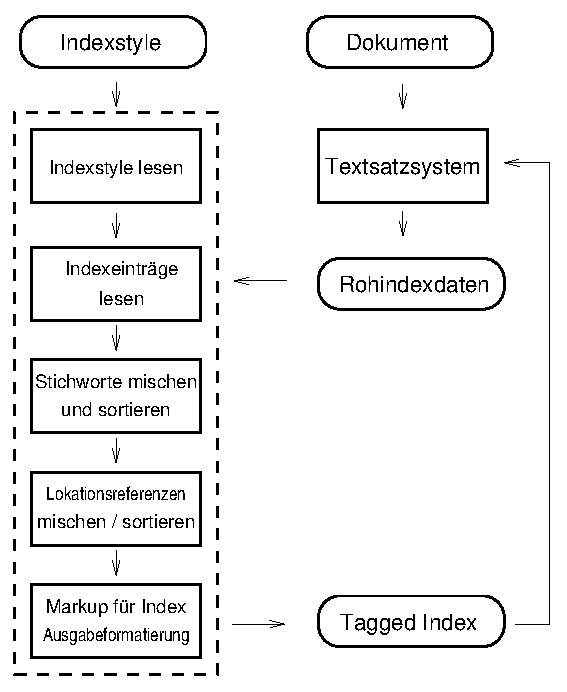
\epsfig{file=datenfluss.eps}
\end{tfigure}


%% Local Variables:
%% mode: latex
%% TeX-master: "makeindex4.tex"
%% End:

%%
%% $Log$
%% Revision 1.2  1995/10/20 11:57:32  kehr
%% Korrektur nach Klaus' Durchsicht.
%%
%% Revision 1.1  1995/10/16  17:31:50  kehr
%% Initial checkin of Report and Presentation.
%%
%% Revision 1.18  1995/10/06  23:05:12  kehr
%% Korrektur nach der Durchsicht von Karin.
%%
%% Revision 1.17  1995/09/22  01:12:01  kehr
%% Zweite �berarbeitung nch der inhaltlichen Korrektur. Au�erdem habe
%% ich das Logo zu MacIndex ver�ndert. Hat jetzt mehr pepp !
%%
%% Revision 1.16  1995/09/21  00:05:42  kehr
%% Erste Ver�nderungen nach der inhaltlichen Korrektur durch Joachim am
%% 20.Sep.95. Fast alle Dateien d'sind davon betroffen. Au�erdem sind noch zwei
%% neue Abbildungen hinzugekommen.
%%
%% Revision 1.15  1995/09/06  18:52:48  kehr
%% Made final changes before giving for correction.
%%
%% Revision 1.14  1995/08/28  18:08:12  kehr
%% Neue Einspielung der xfig-Dateien
%%
%% Revision 1.13  1995/07/04  09:46:28  kehr
%% Weitere �nderungen. Bin aber fast fertig.
%%
%% Revision 1.12  1995/07/04  00:46:48  kehr
%% Bald ist's soweit ;-)
%% Ich habe heute die generelle Umstrukturierung vorgenommen und einige
%% Teile herausgeschmissen. Die Indexverarbeitung mu� noch �berarbeitet werden.
%%
%% Revision 1.11  1995/06/17  20:36:28  kehr
%% Habe die Lokationsreferenzverarbeitung umstrukturiert und besser
%% definiert. DIe Buchstabengruppen m�ssen noch beendet werden und der
%% Algorithmus zum Mischen und Sortieren der Lokationsreferenzen mu�
%% fertiggestellt werden.
%%
%% Revision 1.10  1995/06/09  20:59:48  kehr
%% Superviel gemacht heute ;-)
%%
%% Revision 1.9  1995/06/08  20:19:46  kehr
%% Bibliographie erweitert.
%%
%% Revision 1.8  1995/06/08  00:35:53  kehr
%% Was soll ich blo� schreiben ???
%%
%% Revision 1.7  1995/05/31  19:18:51  kehr
%% Fertigstellung des Analyse-Abschnitts (Hoffentlich ;-).
%%
%% Revision 1.6  1995/05/29  00:22:42  kehr
%% Die Einleitung ist somweit fertig und die Analyse mu� jetzt noch
%% beendet werden. Mir fehlt da noch eine vern�nftige Idde f�r die
%% Alphabete und deren Definitionen.
%%
%% Revision 1.5  1995/05/28  21:37:09  kehr
%% Neue �berarbeitete Version.
%% Inhaltliche �nderungen:
%%   Glossar hinzugenommen. Einleitung mit Datenflu�graph. Kleinere
%%   �nderungen an der Beschreibung des International Makeindex.
%% System�nderungen:
%%   Makefile-�nderungen, Stil�nderungen, Titelseite
%%
%% Revision 1.4  1995/05/05  22:25:03  kehr
%% Ge�nderte Struktur mit einleitung.tex
%% Zwischenspeicherung vor der Umstellung der Definitionen
%%
%% Revision 1.3  1995/04/30  16:14:09  kehr
%% Trennung in Einleitung, Einf�hrung und Analyse. Evtl. sollten die Filenamen
%% entsprechend anepa�t werden. Dar�berhinaus Analyse weitergef�hrt.
%%
%% Revision 1.2  1995/04/25  01:09:39  kehr
%% Analyse und Modellentwurf weitergebracht.
%%
%% Revision 1.1  1995/04/22  21:05:39  kehr
%% Erstes Setup der Studienarbeit des Makeindex4-Projektes
%%



%%
%% $Id$
%%
%% Document: Analyse der Indexverarbeitung `makeindex4' - Projekt
%%

\chapter{Grundanalyse und Begriffsdefinitionen}
\label{sec:analyse}


In diesem Abschnitt werden die grunds�tzlichen Aspekte und Verfahren
der Indexverarbeitung zusammengefa�t und die Funktionsweisen
verschiedener Systeme untersucht. Um einen leichteren Einstieg in die
generelle Problematik der Indexverarbeitung zu erreichen, nehmen wir
als Beispiel einen Index, anhand dessen wir die prinzipiellen
Grundgedanken der Indexverarbeitung vermitteln wollen.


\section{Stichwort}

%\afterpage{%
  \begin{tfigure}%
    {Index mit Seitennummern aus einem Sachbuch �ber Algorithmen}%
    {fig:indEinleitung}%
    \centering%
    \begin{minipage}{9cm}%
      \begin{mkindex}
        \idx B�ume
        \subidx AVL, \textbf{23}, 22--25, 38
        \subidx nat�rliche, {\bfseries 20}, 18--21
        \idx Fibonacci Queues, \emph{siehe} Priority Queues
        \idx Suche
        \subidx bin�re, {\bfseries 5}, 4--7, 11
        \subidx sequentielle, {\bfseries 7}, 6--8, 10
        \subidx geordnete, 6, \emph{siehe auch} ungeordnete Suche
        \subidx ungeordnete, 7
        \idx Priority Queues
        \subidx Fibonacci, {\bfseries 35--36}, 41\emph{f.}%
      \end{mkindex}%
    \end{minipage}%
  \end{tfigure}%
%}

\remark{Hierarchische Struktur}%
Wir untersuchen nun anhand eines Beispielindexes die Grundstruktur von
Indexen. Schauen wir uns Abbildung~\ref{fig:indEinleitung} an, so
k�nnen wir allgemein sagen, da� ein Index eine hierarchisch
gegliederte, vertikal angeordnete und sortierte Struktur aus
Stichw�rtern und Unterstichw�rtern mit jeweils dazugeh�rigen
Referenzen wie Seiten- und Abschnittsnummern ist. Unter einem
\emph{Stichwort}\remark{Stichwort} verstehen wir einen hierarchisch
untergliederten Begriff wie \zB \sym{B�ume, nat�rliche}. Die Struktur
von Stichw�rtern ergibt sich aus der
\emph{vertikalen}\remark{Vertikale Anordnung} Anordnung, in welche die
Unterstichpunkte gem�� vorgegebener Sortierreihenfolge eingeordnet
werden. Im folgenden verwenden wir die Notation
%
\begin{center}
{\tt (}
    \Arg{Ebene$_{1}$} {\tt :} \Arg{Ebene$_{2}$} {\tt :}
    \ldots{} {\tt :} \Arg{Ebene$_{n}$}
{\tt )}\ ,
\end{center}
%
\noindent um die hierarchische Untergliederung von Stichw�rtern zu
beschreiben. In dieser Notation werden Ebenen durch Doppelpunkte
getrennt, und ihre oberste Gliederungsstufe wird zuerst angef�hrt. Die
einzelnen Hierarchieebenen eines Stichworts bestehen aus
Zeichenketten. Wir werden in Abschnitt \ref{def:Zeichenkette} noch auf
die genaue Definition einer Zeichenkette eingehen.

\section{Lokationsreferenz}

Zu jedem Stichwort geh�rt eine Menge von
\emph{Lokationsreferenzen}\remark{Lokationsreferenz}. Diese Referenzen
liegen in einer \emph{horizontalen} Anordnung vor.  Im Beispiel
besitzt das Stichwort \Hierzwei{B�ume}{nat�rliche} die Referenzmenge
$\{\mbox{\bfseries 20}, \mbox{18--21}\}$. Die optische Hervorhebung
der Seitennummer \sym{20} wird oft benutzt, um auf besonders wichtige
Stellen im Text hinzuweisen. Im folgenden wird der Begriff
\emph{Referenz}\remark{Referenz} nahezu synonym zu
\emph{Lokationsreferenz} und \emph{Lokation}\remark{Lokation}
verwendet, da wir im weiteren nicht zwischen der Lokation selbst (also
einer bestimmten Seite oder einem Abschnitt in einem Dokument) und der
Referenz auf diese Lokation (\zB aus dem Stichwortverzeichnis heraus)
im einzelnen unterscheiden m�ssen.\footnote{Trotzdem benutzen wir den
  Begriff \emph{Lokation} eher dann, wenn die reale Lokation --- also
  die Seite oder der Abschnitt --- gemeint ist.}

Lokationsreferenzen wie \sym{\ldots\emph{siehe}\ldots} oder
\sym{\ldots\emph{siehe auch}\ldots} bilden einen speziellen Typ von
Referenzen. Diesen Referenztyp bezeichnen wir mit
\emph{Verweisreferenz}. \remark{Verweisreferenz} Eine Verweisreferenz
besteht aus einem Typ (\emph{siehe}, \emph{siehe
  unter}, \emph{siehe auch} \etc) und dem verwiesenen Stichwort,
welches wir mit \emph{Verweisstichwort} \remark{Verweisstichwort}
bezeichnen. Wir notieren Verweisreferenzen in der Form
\begin{center}
  \VwRef{\Arg{Verweisart}}{\Arg{Verweisstichwort}}.
\end{center}
Im Beispiel ist also bei \VwRef{\emph{siehe}}{Priority Queues}
\sym{\emph{siehe}} der Verweisreferenztyp und \sym{Priority Queues}
das zugeordnete Verweisstichwort.

\remark{Attributierte Lokationsreferenz}%
Die Referenz \sym{41\emph{f.}} aus unserem Beispiel bildet noch einen
weiteren Referenztyp. Hierbei handelt es sich um eine Lokation, der
noch ein zus�tzliches Attribut zugeordnet ist. Die Schreibweise
\sym{\Arg{Lokation}\emph{f.}} bezeichnet in einem Index �blicherweise
einen Verweis auf die angegebene und die ihr folgenden Seiten \bzw
Lokationen. Die beigef�gte Markierung \sym{\emph{f.}} stellt damit
eine zus�tzliche Eigenschaft einer Referenz dar. Da es sich um ein der
Lokation zugeordnetes Attribut handelt, bezeichnen wir diesen
Lokationstyp im folgenden als \emph{Attributierte Lokationsreferenz}.
Wir werden sp�ter noch weitere solcher Attribute einf�hren. Zun�chst
jedoch definieren wir auch hier eine eigene Notation der Form
\begin{center}
  \AttrStruk{\Arg{Lokationsreferenz}}{\Arg{Attribut}}
\end{center}
f�r diese Referenzart.

\remark{Bereiche}%
�blicherweise fa�t man aufeinander folgende Lokationsreferenzen zu
einem \textit{Bereich} zusammen. Solche Bereiche findet man meistens
in der Form \Arg{Lok$_1$}--\Arg{Lok$_2$}. Ein Bereich stellt damit die
Abk�rzung einer Liste von Lokationsreferenzen dar. In unserem Beispiel
hat das Stichwort \Hierzwei{B�ume}{nat�rliche} den Bereich 18--21.
Wir verwenden im folgenden die Notation
\begin{center}
  \Range{Lok$_1$}{Lok$_2$} ,
\end{center}
um einen Bereich zu notieren.

\section{Indexklassen}
\label{sec:ana:Indexklassen}

Nach den Betrachtungen zu Stichw�rtern und Lokationsreferenzen wenden
wir uns dem Thema \emph{Indexklassen}\remark{Indexklassen} zu.
Umfangreichere wissenschaftliche Werke besitzen heute neben einem
Stichwortverzeichnis h�ufig noch Indexe f�r Autoren, Symbole \etc\ In
\cite{griechen} werden beispielsweise insgesamt vier verschiedene
Indexe unter den Oberbegrif"|fen \emph{Mythologische Namen},
\emph{Geographische Namen}, \emph{W�rter} und \emph{Sachen} gef�hrt.
Separate Indexe f�r Befehle und Kommandos sind in vielen technischen
Handb�chern �blich. Diese verschiedenen Indexe sind dar�ber hinaus
noch nach Bedarf unterschiedlich im Layout, k�nnen aber prinzipiell
aus einem einzigen Ursprungs-Datenstrom von Indexeintr�gen stammen.
Unser Modell sollte also die Verarbeitung von verschiedenen
Indexklassen mit unterschiedlichen Eigenschaften wie Lokationsklassen,
Ausgabeformatierung \usw{} grunds�tzlich erm�glichen. Jeder
Indexeintrag mu� also Informationen �ber seine Klassenzugeh�rigkeit
enthalten. Eine gleichzeitige Zuordnung zu mehreren Klassen ist
m�glich.  Beispielsweise findet sich zu verschiedenen thematisch
gegliederten Indexen noch ein Gesamt- oder Master-Index, in dem
nochmals alle Begrif"-fe der Teilindexe zusammengefa�t sind.


\section{Stichwortverarbeitung}
\label{sec:ana:Stichwortverarbeitung}

Wie wir bereits in Abschnitt~\ref{sec:ana:Einfuehrung} erw�hnt haben,
f�hrt jedes Stichwort eine Liste von Lokationsreferenzen mit sich. Wir
haben also als Oberordnung eines Indexes die hierarchische Ordnung der
Stichw�rter, die im folgenden beschrieben wird. Die Ordnung der
Lokationsreferenzen wird in Abschnitt~\ref{sec:ana:RefOrdnung}
behandelt.

Dadurch ist der Indexierungsproze� grunds�tzlich in die beiden
Aufgaben \emph{Stichwortverarbeitung} und
\emph{Lokationsreferenzverarbeitung} zerlegbar. Beide Arbeitsprozesse
sind getrennt voneinander durchf�hrbar. Wir analysieren zun�chst die
Mischung und Sortierung von Stichworthierarchien.

\subsection{Hierarchiestruktur}
\label{sec:ana:StwHierarchiestruktur}

An unserem Beispiel in Abbildung~\ref{fig:indEinleitung} ist die
hierarchische Struktur der Stichw�rter of"|fensichtlich zutage
getreten.  Zwar gibt es verschiedene Beispiele f�r Indexe, welche
keine Untergliederung aufweisen, aber solche \emph{flachen} Indexe
sind eher die Ausnahme als die Regel. Es ist aber nicht immer so, da�
die Untergliederung auch in einer entsprechenden optischen
Form sichtbar wird, wie in unserem Beispiel.\remark{Ausgabestile von
  Indexeintr�gen} So definiert das \emph{Chicago Manual of
  Style}~\cite{chicago}%\textsl{Kap.\,18.18}%
\ua{} den Stil \emph{flush-and-hang style}, welcher unserem Beispiel
entspricht, und \emph{run-in indended style}, welcher Substrukturen
nicht explizit optisch hervorhebt, um dadurch eine Platzersparnis zu
erreichen.  Weitere Arten von unterschiedlichen Ausgabestilen wie \zB
in \cite{BGB} sind dar�ber hinaus denkbar.

Prinzipiell �ndert sich aber nur die Art der Ausgabe des fertigen
Indexes. Dieser Vorgang wird �blicherweise als
\emph{Ausgabeformatierung} bezeichnet und meint das Anheften von
Formatierungsinformationen an den generierten Index, aus welchem dann
das Satz-, Text- oder Informationssystem ein formatiertes Dokument
erzeugt.


\subsection{Sortieren und Mischen von Stichw�rtern}
\label{sec:ana:StwSortierung}

Als grunds�tzliches Problem stellt sich nun die Frage nach der
Sortierung der Stichw�rter. In \cite{chicago}%\textsl{Kap.\,18.98}%
und \cite{Lamb:EPODD-6-1-23} wird auf die Alphabete eines Indexes und
damit auf die Ordnungsrelationen zwischen Stichw�rtern eingegangen.
Die Sortierungsfrage wird dort durch das Beispiel von englischen \bzw
amerikanischen Sortierregeln aufgeworfen.\remark{nationale
  Sortierregeln} Als Beispiel wird das Stichwort \quasi{St.\ Louis}
nach amerikanischen Sprachregeln so sortiert, als ob es ausgeschrieben
w�rde. Es taucht also im Index an der Position von \quasi{Saint Louis}
auf. Es werden weitere Beispiele f�r die Einsortierung von Namen in
einen Index aufgef�hrt, wobei man als Beispiel entsprechende
Sortierregeln f�r das Spanische und Vietnamesische analysiert.
Grunds�tzlich l��t sich also festhalten, da� die Sortierung der
Stichw�rter von Sprachen und deren orthographischen Regeln abh�ngt.

Im \Makeindex-System%~\cite{Chen:SPE-19-9-897}%
wird das Problem teilweise gel�st, indem zum Sortierschl�ssel
\emph{sort key} ein weiterer Druckschl�ssel\remark{Druckschl�ssel}
\emph{actual key} eingef�hrt wird, welcher beim der abschlie�enden
Ausgabeformatierung den Sortierschl�ssel substituiert. Dieses
Verfahren umgeht die \quasi{St.\ Louis}-Problematik, indem man in
einem solchen Fall die Substitution separat angibt, ist aber
prinzipiell sehr unbequem zu handhaben.  Man bedenke, da� in der Regel
viele spezielle nationale Zeichens�tze\remark{nationale Alphabete} mit
Umlauten nicht innerhalb des lateinischen Alphabets sortierbar sind.
Nach deutschen Orthographieregeln wird der Buchstabe \quasi{�} je nach
Fall wie \quasi{ae} oder auch wie \quasi{a} einsortiert. Es gibt also
noch nicht einmal einheitliche Standardregeln, nach denen ein
Indexierungssystem sortieren k�nnte. F�r alle diese Stichw�rter immer
separat den Druckschl�ssel angeben zu m�ssen, ist f�r den Benutzer
eine unakzeptable L�sung.

In \emph{International MakeIndex}~\cite{Schrod:CG-10-81} wird die
Problematik durch ein regelbasiertes Substitutionsschema angegangen.
Innerhalb dieses Substitutionsschemas k�nnen Sortierregeln f�r
beliebige Alphabete angegeben werden. Dort kann der Benutzer Regeln
definieren, um in einem deutschen Text den Buchstaben \quasi{�} vor
der Sortierung \zB auf die Buchstaben \quasi{ae} abzubilden. Diese
Regeln werden verwendet, um aus dem Stichwort einen Sortierschl�ssel
zu generieren, welcher implizit zur Sortierung verwendet wird. Die
Abbildung des Stichworts in den Sortiersch�ssel wird als \emph{sort
  mapping}\remark{sort mapping} bezeichnet. Dar�ber hinaus ist dieses
Konzept allgemein genug, da� es auch auf die Sortierung von Zahlen,
Symbolen, Formeln \etc angewendet werden kann. Sollten diese Regeln in
Einzelf�llen nicht gen�gen, so kann immer noch auf die explizite
Angabe des Sortierschl�ssels ausgewichen werden.

Durch die Einf�hrung der Sortierungsabbildung treten weitere
grunds�tzliche Probleme auf, die durch die zus�tzliche Einf�hrung
einer Mischabbildung (\emph{merge mapping}\remark{merge mapping})
gel�st werden konnten. Sie generiert auf analoge Weise einen
Mischschl�ssel, der entscheidet, welche Eintr�ge als \Quasi{gleich}
angesehen werden.  Man erreicht mit dieser Abbildung eine
\emph{Normalisierung}\remark{Normalisierung} des Mischschl�ssels, um
von einer konkreten Repr�sentation eines Schl�ssels zu einer
abstrakten Repr�sentation zu gelangen. Eine ausf�hrliche technische
Beschreibung der beiden Abbildungsverfahren findet sich in
\cite{Schrod:Makeindex30}.

Eine M�glichkeit, den Index zu erweitern, besteht in der Hinzunahme
von \emph{Permutierten Indexschl�sseln}\remark{Permutierter
  Index}.\label{index:permutierter} Darunter versteht man das
automatische Generieren eines Stichwortes \Hierzwei{bin�re}{Suche} aus
dem Stichwort \Hierzwei{Suche}{bin�re} durch Wortpermutationen. Diese
sind in \cite{Bentley:EPODD-1-1-3} implementiert, gelingen jedoch
teilweise lediglich deshalb, weil die englische Sprache eine
Permutation \zB von \quasi{\textsl{sorting a book index; a book index,
    sorting; book index, sorting a; index, sorting a book\/}} erlaubt,
diese jedoch nicht ohne weiteres auf die deutsche oder andere Sprachen
�bertragbar ist.


\section*{Zusammenfassung}%
Wir haben also anhand unseres Beispiels festgestellt, da� ein Index
eine hierarchische Struktur besitzt.  Wir haben eine vertikale
Struktur von Stichw�rtern und eine horizontale Struktur von
Lokationsreferenzen erkannt und grunds�tzlich dargelegt.  Des weiteren
haben wir verschiedene Lokationstypen ausgemacht.  Diese Typen werden
im sp�teren Verlauf als Lokationsklassen weiterbehandelt werden.
Lokationsreferenzen k�nnen bestimmte Attribute zugeordnet werden. Wir
unterscheiden attributierte Lokationsreferenzen und Verweisreferenzen.

%%Die Sortierung der Stichw�rter unterliegt sehr stark dem intuitiven
%%Verst�ndnis des Menschen von alphabetischer Ordnung und
%%Strukturierung. Der Leser w�nscht sich einen Index, in welchem er
%%gew�nschte Informationen m�glichst schnell und ef"|fektiv findet. Diese
%%Vorgaben f�hren konsequenterweise zu einer einfachen, hierarchischen
%%und �bersichtlichen Struktur der Stichw�rter.


\chapter{Analyse}
\label{sec:ana:Lokationsreferenzen}
\label{sec:ana:RefOrdnung}

\section{Strukturelle Analyse}

\subsection{Klassen von Lokationsreferenzen}
\label{sec:klassenlokationsreferenzen}

Nachdem wir uns einen �berlick �ber die Stichw�rter verschafft haben,
gehen wir nun dazu �ber, die Lokationen in vertiefter Weise zu
untersuchen. Hierzu greifen wir unseren Index aus
Abbildung~\ref{fig:indEinleitung} auf und erweitern ihn mit neuen
Lokationsreferenzen, anhand derer wir den Lokationsbegriff neu
klassifizieren. Um den Blick auf das Wesentliche zu lenken, sind die
Seitennummern des vorigen Indexes gr��tenteils entfernt worden. Der so
ver�nderte Index ist in Abbildung~\ref{fig:indErweitert} dargestellt.

\begin{tfigure}%
  {Index mit Abschnittsnummern aus einem Sachbuch �ber Algorithmen}%
  {fig:indErweitert}%
  \centering%
  \begin{minipage}{9cm}%
    \begin{mkindex}
      \idx B�ume
      \subidx AVL, {\sffamily 2.3}
      \subidx nat�rliche, A-1, {\sffamily 2.1}
%%      \idx Fibonacci Queues, \emph{siehe} Priority Queues
      \idx Suche
      \subidx bin�re, 11, 11a, {\sffamily 1.3}
      \subidx sequentielle, A-2, {\sffamily 1.2}
%%      \subidx geordnete, {\sffamily 1.2.1}, \emph{siehe auch} ungeordnete Suche
      \subidx ungeordnete, {\sffamily 1.2.2}
      \idx Priority Queues
      \subidx Fibonacci, {\sffamily 3.3}
    \end{mkindex}%
  \end{minipage}%
\end{tfigure}
%
Wie man sehen kann, sind in diesen Index Abschnittsnummern neu
hinzugekommen. Abschnittsnummern (hier \textsf{serifenlos} gedruckt)
bilden eine weitere M�glichkeit auf Lokationen innerhalb eines
Dokuments zu verweisen.
\remark{Hierarchien\-struktur}%
Die Abschnittsgliederung \quasi{{\sffamily 2.1}} ist eine hierarchisch
in Kapitel und Abschnitt zerlegte Lokation mit dem Trennzeichen
\quasi{{\sffamily .}}$\:$. Die Referenz \quasi{\mbox{A-1}} ist
gleichfalls eine mehrstufige Referenz. Sie bildet sich aus dem
Buchstaben \quasi{A} (sie soll auf den Anhang des Buches verweisen)
und der Nummer des Abschnitts (in diesem Fall~\quasi{1}). Dieses
Beispiel demonstriert die Unterschiedlichkeit\remark{Unterschiedliche
  Lokationstypen} von Lokationstypen. Eine Lokation bezeichnet eine
bestimmte Dokumentstelle. Ein Dokument kann von verschiedenen
Lokationsstrukturen durchzogen sein. Beispielsweise l��t sich ein
Dokument nach Seiten einteilen, was eine
\emph{externe}\remark{externe} --- also nicht dem Dokument
innewohnende --- Strukturierung darstellt. Im Gegensatz dazu bilden
Gliederungen eine \emph{interne}\remark{interne Dokument\-struktur},
das Dokument betreffende Strukturierung. Auf welche Weise nun auf ein
Dokument verwiesen werden soll, ist insbesondere eine Frage, ob auf
die interne oder externe Struktur oder beides verwiesen werden soll.

Die Verschiedenheit von Lokationen wird in den untersuchten Systemen
\cite{Chen:UCB-TR-87-347,starwriter,winword,Bentley:EPODD-1-1-3,Lamb:EPODD-6-1-23}
nicht beachtet. Diese Systeme sind nur in der Lage, Seitennummern und
Verweisreferenzen %%wie \VwRef{Fibonacci Queues}{Priority Queues}%%
zu verwalten. Hierzu finden sich weitere Lokationstypen:

Beispielsweise werden im \emph{System Management
  Guide}~\cite{AIXmanual} die Seitennummern kapitelweise gez�hlt, so
da� sich die Seitennummern aus einer zweistufigen Nummer der Form
\quasi{\Arg{Kapitel}--\Arg{Kapitelseite}} wie \zB{} \quasi{7--13}
bilden.
%F�r diese Numerierung versagen die \oa{} Systeme, da
%sie nicht in der Lage sind Strukturen und Hierarchien innerhalb von
%Lokationen zu verarbeiten.

Des weiteren ist die Referenz auf Seite \quasi{11a} des Stichworts
\Hierzwei{Suche}{bin�re} auch eine hierarchisch strukturierte
Lokationsreferenz. H�ufig werden Manuals durch Hinzunahme von Seiten
wie \quasi{11a} erweitert, um bei nachtr�glichen Korrekturen die
urspr�ngiche Seitenfolge nicht zu st�ren. Dabei sollen bei
verschiedenen Versionen eines Manuals m�glichst alle Numerierungen
gleichbleibend sein.
%%Beispiel f�r ein solches Manual ist \cite{AIXmanual}.

Im juristischen Umfeld gibt es h�ufig B�cher, die nach Gesetzb�chern
und Paragraphen strukturiert sind \cite{BGB}. Dort wird nach den
Stichw�rtern die Nummer des Gesetzbuches angegeben und anschlie�end
werden die zugeh�rigen Paragraphen aufgez�hlt. Als Beispiel soll der
folgende Auszug dienen.\footnote{Fette Nummern bezeichnen hier die
  Nummer des Gesetzbuches, w�hrend die normalen Nummern auf die
  zugeh�rigen Paragraphen hinweisen.}
  \label{bsp:BGB}
\begin{center}
  \textbf{Lasten} beim Kauf \textbf{1} \S436, \S446; auf der Mietsache
  \textbf{1} \S546; \ldots
\end{center}

\noindent Grunds�tzlich k�nnen wir also nach diesen Betrachtungen sagen, da�
eine Lokationsreferenz eine hierarchische
Struktur\remark{Lokations\-struktur} aufweist. Die Struktur besteht
aus einzelnen Hierarchieebenen wie Kapitelnummer, Abschnittsnummer
\usw oder zus�tzlichen Aufz�hlungen wie \quasi{11}, \quasi{11a}.
Dr�cken wir diese Hierarchiestruktur auch durch eine spezielle
Notation aus, so m�ssen wir beachten, da� hierbei noch Trennzeichen
wie Bindestriche oder Punkte zwischen den Hierarchien auftreten
k�nnen. Wir definieren also die Notation
\begin{center}
\Strukvier{\textsl{Ebene$_{1}$}}{\textsl{Trenner$_{1}$}}%
        {\textsl{Ebene$_{2}$}}{\textsl{Trenner$_{2}$}}%
        {\ldots{}}     {\textsl{Trenner$_{n-1}$}}%
        {\textsl{Ebene$_{n}$}} ,
\end{center}
um eine Hierarchie von Lokationen zu beschreiben. In dieser Notation
wird die Lokation \textsf{1.2.2} als
\textsf{\Strukdrei{1}{.}{2}{.}{2}} geschrieben. Im folgenden
bezeichnen wir diesen Typ von Lokationsreferenz mit
\emph{Strukturreferenz}\remark{Strukturreferenz}. Eine
Strukturreferenz besteht aus allen Hierarchieebenen inklusive der
Trennzeichen. Des weiteren bezeichen wir eine Ebene einer
Strukturreferenz mit \emph{Strukturebene}.


\subsection{Alphabete}
\label{sec:alphabete}

Wir haben im vorangehenden Abschnitt die Struktur der
Lokationsreferenzen dargelegt und wollen uns jetzt mit der Zuordnung
von Lokationsreferenzen zu Lokationsklassen befassen. Da unser System
--- wie man aus dem Datenflu�diagramm in
Abbildung~\ref{fig:datenfluss} erkennen kann --- nichts �ber die
Interna des Textsatzsystems wei�, mu� unser System in der Lage sein,
aus Zeichenfolgen mittels der Angaben im Indexstyle die
Lokationsreferenzen zu erkennen. Wir bezeichnen das der
Indexverarbeitung zugrundeliegende Alphabet von Zeichen als das
\emph{Dokumentalphabet}\remark{Dokument\-alphabet}. Dieses Alphabet
ist der gemeinsame Zeichenvorrat des Satzsystems und des
Indexsystems.\footnote{�blicherweise wird dort das ASCII-Alphabet, die
  ISO-Latin--Familie oder Unicode~\cite{Unicode:US91} Verwendung
  finden.} Die Rohindexdaten und damit auch die Lokationsreferenzen
liegen also im Format dieses Dokumentalphabets vor, und das
Indexsystem mu� daraus die Lokationsreferenzen in ihre Struktur
zerlegen.

Wir unterscheiden die einzelnen Strukturkomponenten einer Lokationsreferenz
in zwei Kategorien:
%
\begin{enumerate}
\item \emph{Aufz�hlbare Typen} wie \zB Seiten-, Abschnitts-  oder
  Kapitelnummern.
\item \emph{Endliche Typen} wie \zB alphabetische Aufz�hlungen von
  Abschnitten. So enth�lt die Lokationsreferenz
  \Strukzwei{Anhang}{--}{A} in der zweiten Strukturkomponente das
  Alphabet der Gro�buchstaben.
\end{enumerate}
%
Wir definieren also zusammenfassend:

\begin{Def}
  Ein \emph{Dokumentalphabet} ist eine endliche Menge von Zeichen.%
  \label{def:dokumentalphabet}%
\end{Def}

\begin{Def}
  Ein \emph{Symbol} ist ein Wort �ber einem Dokumentalphabet.%
  \label{def:symbol}%
\end{Def}

\begin{Def}
  Eine \emph{Aufz�hlung} ${\cal I}$ ist eine unendliche linear
  geordnete Menge von Symbolen. Insbesondere existiert eine bijektive
  Abbildung\ \mbox{$\psi: {\cal I} \rightarrow $ \mathZ{}} des
  Alphabets auf die Menge \mathZ{} der Ganzen Zahlen oder der Menge
  \mathN{} der Nat�rlichen Zahlen.%
  \label{def:aufzaehlung}%
\end{Def}

\begin{Def}
  Ein \emph{Alphabet} ${\cal A}$ ist eine endliche Aufz�hlung von
  Symbolen. Insbesondere existiert eine bijektive Abbildung $\phi :
  {\cal A} \rightarrow $ \mathN{} des Alphabets auf ein endliches
  Intervall
  der Nat�rlichen Zahlen.%
  \label{def:alphabet}%
\end{Def}

\newcommand{\mq}[1]{\mbox{\quasi{#1}}}

\noindent Wir folgern daraus:
%
\begin{Lem}
  Die Strukturkomponenten einer Lokationsreferenz bestehen aus Symbolen.
\end{Lem}
%
\newcommand{\SalphaSymbol}{{\cal S}}%
\newcommand{\Salpha}[2]{\mbox{\(\SalphaSymbol{}^{#1}_{#2}\)}}%
\newcommand{\Dalpha}[1]{\mbox{\({\cal D}_{#1}\)}}%
\newcommand{\TotOrd}[1]{\mbox{\(\sigma_{#1}\)}}%
%
Betrachten wir als Beispiel Seitennummern im Dokumentalphabet
\Dalpha{} vom Typ ISO-Latin, so ist die Seitennummer~\quasi{13} ein
Wort des Dokumentalphabets und damit nach Definition~\ref{def:symbol}
ein Symbol. Die Seitennummern bilden sich nun aus einer Untermenge
\Dalpha{sn} $= \{\mq{0},\ldots,\mq{9}\}$\footnote{also die der
  Zif"|fern des arabischen Zahlensystems} des Dokumentalphabets
\Dalpha{}. Die Menge aller Worte �ber \Dalpha{sn} bilden nach
Definition~\ref{def:aufzaehlung} eine Aufz�hlung. Wir definieren:
%
\newcommand{\TotOrdSortAlphabet}{%
  \mbox{$<_{\mbox{\scriptsize\textit{alph}}}$}\xspace}%
%
\begin{Def}
  \label{def:sortierungsalphabet}
  Ein \emph{Sortierungsalphabet} \Salpha{}{} ist eine Aufz�hlung oder
  ein Alphabet. Die Symbole des Sortierungsalphabets sind W�rter �ber
  einer Untermenge \Dalpha{\SalphaSymbol} $\subseteq$ \Dalpha{} des
  Dokumentalphabets.
\end{Def}
%
Wir bringen mit dieser Definition zum Ausdruck, da� ein
Sortierungsalphabet sowohl ein endliches Alphabet (wie die Menge der
Gro�buchstaben) als auch eine unendliche Aufz�hlung (wie im Falle der
Seitennummern) sein kann.
%
\begin{Def}
  \label{def:sortierungsalphabet:ordnung}
  Auf jedem Sortierungsalphabet \Salpha{}{} ist gem�� der
  Definitionen~\ref{def:aufzaehlung} und \ref{def:alphabet} eine
  bijektive Abbildung
  $\TotOrd{\SalphaSymbol}\,:~\SalphaSymbol\,\rightarrow\,\mathZ$
  definiert. Diese Abbildung stellt eine \emph{lineare Ordnung}
  \TotOrdSortAlphabet bez�glich paarweiser Elemente
  $s_1,s_2\in\Salpha{}{}$ auf dem Sortierungsalphabet dar.  Die
  Ordnungsrelation $s_1\,\TotOrdSortAlphabet\,s_2$ gilt genau dann,
  wenn $\TotOrd{\SalphaSymbol}(s_1)\,<\,\TotOrd{\SalphaSymbol}(s_2)$.
  %%Die Menge \Salpha{}{} bildet mit dieser Ordnung einen
  %%\emph{vollst�ndigen Verband} \mbox{$(\SalphaSymbol,
  %%\TotOrdSortAlphabet)$}.
\end{Def}
%
\begin{Def}
  Ein \emph{Basisalphabet} \Dalpha{\SalphaSymbol} eines
  Sortierungsalphabets \Salpha{}{} ist die kleinste Untermenge des
  Dokumentalphabets\, \Dalpha{}, aus der die Worte des
  Sortierungsalphabets\, \Salpha{}{} vollst�ndig gebildet werden
  k�nnen.%
  \label{def:basisalphabet}
\end{Def}

\noindent Betrachten wir nun folgendes Beispiel: Die Strukturreferenz
\Strukzwei{\emph{Gro�buchstabe}}{--}{\emph{Abschnittsnummer}} mit dem
Dokumentalphabet \Dalpha{} hat auf der ersten Strukturkomponente das
Sortierungsalphabet \Salpha{1}{} mit den Symbolen \Salpha{1}{1} $=$
\mq{A},\ \Salpha{1}{2} $=$ \mq{B}, \ldots{}, \Salpha{1}{26} $=$
\mq{Z}.  Daraus ergibt sich das Basisalphabet
\Dalpha{\SalphaSymbol{}^{1}}$\,=\{\mq{A},\ldots,\mq{Z}\}$. Auf der
zweiten Ebene haben wir das Sortierungsalphabet
\Salpha{2}{}$\,=\{\mq{1},\mq{2},\ldots{},\mq{9},\mq{10},\ldots\}$ mit
dem Basisalphabet
\Dalpha{\SalphaSymbol{}^2}$\,=\{\mq{0},\ldots{},\mq{9}\}$.


\subsection{Komponententypen}
\label{sec:basistypen}

Wir betrachten nun diverse
\emph{Komponententypen}\remark{Komponenten\-typen} von
Strukturkomponenten. Ein Komponententyp ist ein Tupel $B = ( {\cal S},
{\cal B} )$ mit ${\cal S}$ Symbolalphabet und ${\cal B}$
Basisalphabet.  Tabelle~\ref{tab:LokationsKomponententypen} zeigt uns
einen Teil der �blicherweise verwendeten Komponententypen. Sie sind
nach Aufz�hlungen und Alphabeten geordnet. Um die Komponententypen mit
einfachen Bezeichnungen zu identifizieren, benennen wir sie auf
geeignete Weise.

\begin{ttable}%
  {Tabelle mit Komponententypen von Strukturkomponenten}%
  {tab:LokationsKomponententypen}%
  \centering
  \begin{tabular}{|l|l|c|c|}

    \hline
    \multicolumn{4}{|c|}{Aufz�hlungen\medrule}\\
    \hline
    \smallrule
    \smallrule\textsl{Komponententyp} & \textsl{Symbolalphabet}&
    \textsl{Basisalphabet} & \textsl{Name}\\
    \hline

    numerisch & 0, 1,\ldots, 10,\ldots & $\{0\ldots 9\}$ & \Lokklasse{num}\\

    r�misch (klein) & i, ii,\ldots,x, \ldots & $\{$i,v,x,l,c,d,m$\}$ &
    \Lokklasse{roman}\\

    r�misch (gro�)  & I, II,\ldots,X,\ldots& $\{$I,V,X,L,C,D,M$\}$ &
    \Lokklasse{ROMAN}\\

    Indexaufz�hlung & $x_{1}, x_{2},\ldots, x_{9},\ldots$ & $\{x,
    0,\ldots,9\}$ &\\

    \hline
    \multicolumn{4}{c}{}\\
    \hline

    \multicolumn{4}{|c|}{Alphabete\medrule}\\
    \hline
    \smallrule\textsl{Komponententyp} & \textsl{Symbolalphabet}&
    \textsl{Basisalphabet} & \textsl{Name}\\
    \hline

    alphabetisch (klein) & a, b, c,\ldots, z & $\{$a,\ldots,z$\}$ &
    \Lokklasse{alpha}\\

    alphabetisch (gro�) & A, B, C,\ldots, Z & $\{$A,\ldots,Z$\}$ &
    \Lokklasse{ALPHA}\\

    griechisch (klein) & $\alpha, \beta, \gamma, \delta,\ldots,
    \omega$ & $\{\alpha,\ldots,\omega\}$ & \\

    & {\small Kapitel, Anhang} & {\small $\{$a,A,e,g,h,i,K,l,n,p,t$\}$} &\\
    \hline%
  \end{tabular}%
\end{ttable}

Grunds�tzlich mu� f�r jeden Basishierarchietyp eine Ordnung definiert
sein, damit man die Elemente des Typs in einer numerischen Form
sortieren kann. Aus den Definitionen \ref{def:aufzaehlung} und
\ref{def:alphabet} geht bereits hervor, da� entsprechende Abbildungen
von der Symbolmenge auf eine Zahlenmenge definiert sein m�ssen. F�r
arabische und r�mische Zif"|fernfolgen ist diese Abbildung bereits
durch das �blicherweise benutzte Zahlensystem gegeben.\footnote{Man
  beachte, da� die \oa \quasi{Zahlen} zun�cht einmal nur Zeichenfolgen
  (also Worte �ber dem Dokumentalphabet) darstellen, deren Abbildung
  in das Zahlensystem zuerst definiert werden mu�.} Die hier
aufgef�hrten Komponententypen decken bereits einen Gro�teil aller
Erfordernisse ab. Trotzdem m�ssen wir zulassen, da� besondere
Alphabete, wie das griechische Alphabet oder die numerische
Indexierung, prinzipiell benutzerdefinierbar und frei verwendbar sind,
auch wenn deren Verwendung nur in Spezialf�llen n�tig sein wird.

Wesentlich h�ufiger dagegen ist die Verwendung von festgelegten Worten
wie \quasi{Kapitel}, \quasi{Anhang}, \quasi{Glossar} \usw als
Symbolalphabet, welche in unserer Hierarchieebene ebenfalls eine Ebene
belegen k�nnen. Hierbei mu� dann ebenfalls eine geeignete
Ordnungsrelation definiert werden. Dies k�nnte durch eine einfache
Aufz�hlung der Symbole geschehen wie in der letzten Zeile der Tabelle
dargestellt. Dort sind die Worte \quasi{Kapitel} und \quasi{Anhang}
Symbole des Symbolalphabets, denen aufgrund der Aufz�hlungsreihenfolge
eine Ordnungsrelation zugewiesen wurde.\footnote{Insbesondere kann man
  auch Trennzeichen als Alphabete ansehen, die nur aus einem einzigen
  Symbol bestehen.}


\subsection{Komposition}


Aus den Komponententypen bilden wir nun durch Komposition die
Lokationsklassen. \remark{Lokationsklassen}Mit ihnen beschreiben wir
dem System die Struktur der vorkommenden Lokationsreferenzen und
k�nnen die Erkennung und Zuordnung von Zeichenstr�men zu
Lokationsreferenzen formal beschreiben.

Betrachten wir erneut die in der Praxis verwendeten Lokationstypen, so
k�nnen wir grunds�tzlich die folgenden beiden Klassen unterscheiden:
\begin{enumerate}
\item \emph{Standardklassen},\remark{Standardklassen} deren Struktur
  immer gleich ist, wie \zB Seitennummern der Form
  \Strukeins{\texttt{num}}.
\item \emph{Varklassen},\remark{Varklassen} deren Struktur sich
  variabel aus mehreren Strukturkomponenten zusammensetzt. Dazu
  geh�ren Gliederungsnummern der Form
  \Braces{\Strukebene{\texttt{num}}\texttt{.}\Strukebene{\texttt{num}}\texttt{.}\Strukebene{\texttt{num}}\ldots}.
  Beispielsweise geh�ren die Lokationsreferenzen \Strukeins{2},
  \Strukzwei{2}{.}{1} und \Strukdrei{2}{.}{1}{.}{4} der gleichen
  Gliederungsstruktur an. Man kann hier auch argumentieren, da� jede
  der vorkommenden Strukturen eine eigene Lokationsklasse bildet.
  Prinzipiell bilden diese Varklassen jedoch eine Menge von
  Lokationsklassen, denen wir in den folgenden Abschnitten noch
  weitere gemeinsame Eigenschaften zuordnen k�nnen.
\end{enumerate}
Um dem System ad�quate Beschreibungen zu liefern, m�ssen wir ihm f�r
jede Klassendefinition deren Typ --- Standard- oder Varklasse ---
mitteilen, da wir f�r beide Klassen unterschiedliche
Zuordnungsstrategien anwenden m�ssen.

Wir werden im folgenden die Standard-Lokationsklassen analog zur
Schreibweise von Lokationsreferenzen in der Form
\Strukzwei{\texttt{num}}{\texttt{.}}{\texttt{num}} notieren, und die
Varklassen durch das Anf�gen eines \quasi{\texttt{*}} wie in
\Metaclass{\Strukzwei{\texttt{num}}{\texttt{.}}{\texttt{num}}}. Bei
Varklassen wird durch die Strukturdefinition auch gleichzeitig die
maximale Tiefe festgelegt.


%%Aus den Komponententypen lassen sich nun komplette Strukturen zu einer
%%Lokationsklasse zusammen"-stellen. Au�erdem w�nschen wir f�r die
%%Definition von Klassen der Art
%%\Braces{\Strukebene{\texttt{num}}\texttt{.}\Strukebene{\texttt{num}}\texttt{.}\Strukebene{\texttt{num}}\ldots}
%%eine Beschreibungsform, die es erlaubt, am Ende beliebig viele
%%Wiederholungen von Strukturkomponenten zuzulassen. Wir k�nnen damit
%%verschiedene Klassendefinitionen zu einer Varklasse zusammenfassen,
%%der wir besondere Eigenschaften zuordnen k�nnen. Eine Definition einer
%%Klassenstruktur\remark{Klassenstruktur} wird durch folgende
%%grammatikalische Beschreibung vorgenommen:
%%%
%%\begin{center}
%%  \slshape
%%  \begin{tabular}{lll}
%%    locclass    &::=& \verb="("= prefix \opt{postfix}\verb=")"= \\
%%    prefix      &::=& basetype \opt{layerlist}\\
%%    postfix     &::=& \verb="{"= layerlist \verb="}"=\\
%%    layerlist   &::=& \argplus{separator basetype}\\
%%    basetype    &::=& \Lokklasse{num} \verb=|= \Lokklasse{alpha}
%%    \verb=|= \Lokklasse{ALPHA} \verb=|= \Lokklasse{roman} \verb=|=
%%    \Lokklasse{ROMAN}\\
%%    &&\verb=|= \Lokklasse{userdefined} \verb=|= \Lokklasse{empty}\\
%%    separator   &::=& \textbf{String}
%%  \end{tabular}
%%\end{center}
%%%
%%Wir k�nnen mit dieser Beschreibungsform die Strukturkomponenten am Ende
%%klammern und lassen von diesen Ebenen beliebig viele
%%aufeinanderfolgende Wiederholungen zu. Wir k�nnen \zB die Klasse der
%%Abschnittsnummern mit beliebiger Tiefe in Punktnotation eines Dokumentes in der Form
%%%
%%\begin{center}
%%  \Metaclass{\Strukebene{num}}{\texttt{.}\Strukebene{num}}
%%\end{center}
%%%
%%beschreiben.\footnote{Entscheidend ist, da� alle Loaktionsreferenzen
%%  der Form \Lokklasse{num}\textbf{.}\Lokklasse{num}\ldots zur selben
%%  Klasse geh�ren.} Eine dadurch definierte Klasse unterscheidet sich
%%in der Semantik gegen�ber der Definition von separat definierten
%%Lokationsklassen, wie wir im folgenden Abschnitt beschreiben werden.


\subsection{Vertr�glichkeit}

Um Strukturkomponenten zu Hierarchien zu verkn�pfen, mu� die
Komposition von Komponententypen zu einer kompletten Hierarchie
inklusive aller Trennzeichen speziell untersucht werden. Insbesondere
mu� ein System in der Lage sein, einem Zeichenstrom die richtige
Lokationsklasse zuzuordnen.\remark{Zuordnungs\-problem} Die folgenden
Beispiele sollen in die Problemstellung einf�hren:
%
\begin{enumerate}

\item \Strukzwei{\texttt{num}}{\textbf{.}}{\texttt{num}}

  definiert eine Lokationsklasse, deren erste und zweite
  Hierarchiestufe durch arabische Zahlen repr�sentiert werden. G�ltige
  Repr�sentanten dieser Klasse sind beispielsweise die folgenden,
  aufsteigend sortierten Referenzen 1.1, 1.2, 1.3, \ldots{}, 2.0, 2.1,
  \ldots{}, 2.20, \ldots{} .

  Die Sortierung erfolgt demnach streng von der obersten
  Hierarchiestufe bis zur untersten. Insbesondere ist das Trennzeichen
  \quasi{\textbf{.}} unbedingt erforderlich, da sonst nicht zwischen
  den Z�hlebenen unterschieden werden kann (12 kann sein 1.2 oder
  \textsl{zw�lf\/}).

\item \Strukzwei{\texttt{num}}{}{\texttt{roman}}

  definiert eine Aufz�hlungsform, die nicht unbedingt ein Trennzeichen
  verlangt, da das Basisalphabet von \Lokklasse{num} und das der
  r�mischen Zif"|fern \Lokklasse{roman} disjunkt und damit eindeutig
  unterscheidbar sind. Beispiele f�r solche Klassenvertreter sind 1i,
  1ii, 1iii, 1iv, \ldots{}, 2i, \ldots{} .

\item \Strukzwei{\texttt{roman}}{}{\texttt{alpha}}

  In diesem Fall ist das Basisalphabet des Komponententyps
  \Lokklasse{roman} echte Untermenge des Komponententyps
  \Lokklasse{alpha}, da alle r�mischen Zif"|fern ebenfalls Elemente
  des lateinischen Alphabets sind. Im Fall der Zeichenkette
  \quasi{ivi} kann man sowohl auf die Lokationsreferenz
  \Strukzwei{iv}{}{i} als auch \Strukzwei{i}{}{vi} schlie�en, wobei
  letztere genau genommen einen Fehler darstellen w"urde. Man kann
  demnach keine exakte Hierarchieebene ermitteln, wenn keine
  eindeutigen Trennzeichen verwendet werden und die Zeichenmengen
  nicht disjunkt sind.

\end{enumerate}

\smallskip

\noindent Aus diesen �berlegungen k�nnen wir also folgern:

\begin{Lem} Zwei Sortierungsalphabete ${\cal A}$ und ${\cal B}$ sind
  grunds�tzlich miteinander \emph{vertr�glich}, wenn f�r deren
  Basisalphabete \Dalpha{A} und \Dalpha{B} gilt:
  \Dalpha{A}~$\cap$~\Dalpha{B} $=~\emptyset$.
\end{Lem}

\noindent Verwenden wir geeignete Trennzeichen, die mit den Basisalphabeten
der Komponententypen disjunkt sind, so k�nnen wir das
Vertr�glichkeitsproblem\remark{Vertr�glichkeit} explizit umgehen. Alle
Kompositionen von Komponententypen, welche nicht vertr�glich sind,
m�ssen durch implizite Konventionen oder spezielle eindeutige
Festlegungen spezifiziert werden.


\subsection{Zuordnungsstrategien}

Um einen Zeichenstrom anhand der Beschreibungen der Komponententypen und
Lokationsklassen genau einer Lokationsklasse zuzuordnen, m�ssen wir
geeignete Zuordnungsstrategieen entwerfen.

Standard-Lokationsklassen sind duch ihre gleichbleibende Struktur
definiert. Wir verlangen daher, da� ein Zeichenstrom auf alle
Komponententypen und Trennzeichen einer Lokationsklasse passen mu�, um
akzeptiert zu werden. Wir nennen diese Erkennungsstrategie
\emph{Exaktes Zuordnen}\remark{Exaktes Zuordnen}.

Varklassen definieren eine Menge von Lokationsklassen und die
Zuordnungsstrategie mu� in der Lage sein, alle m�glichen Teilklassen
f�r die Zuordnung heranzuziehen. Wir m�ssen daher auch eine
Teil�berdeckung zulassen. Da eine �berdeckung nur streng von links
nach rechts erfolgen kann, sprechen wir im folgenden von einer
\emph{Pr�fix�berdeckung}. Demnach lassen wir hier eine Zuordnung auch
dann zu, wenn ein Zeichenstrom nur auf den Pr�fix einer Varklasse
pa�t. Wir nennen diese Zuordnungsstrategie
\emph{Pr�fixzuordnung}\remark{Pr�fixzuordnung}.

Kombinieren wir beide Lokationsklassentypen derart, da� wir
Lokationsklassen in der allgemeinen Gestalt
\begin{center}
  \Arg{Standard-Hierarchien}\Arg{Var-Hierarchien}
\end{center}
ausdr�cken, so k�nnen wir noch pr�zisere Erkennungsstrategien f�r
bestimmte Lokationsklassen gewinnen. Jeweils einer der beiden
Hierarchieanteile ist dabei optional. Verwenden wir die
Zuordnungsstrategie Exaktes Zuordnen f�r den Pr�fix-Anteil und die
Pr�fixzuordnung f�r den Var-Anteil, so erhalten wir noch einen
dritten, kombinierten Lokationsklassentyp, der aus einer Mischung von
Standard- und Varklassen besteht.

F�r die in der Praxis vorkommenden Lokationsreferenzen reicht die
einfache Beschreibungsform der separaten Standard- und Varklassen
jedoch grunds�tzlich aus und wir werden sie nicht weiter in die
Untersuchungen mit einbeziehen.


\subsection{Zuordnung zu Lokationsklassen}

Verwenden wir Lokationsklassen, die nicht miteinander vertr�glich
sind, so m�ssen wir heuristische Verfahren untersuchen, um trotzdem
eine Zuordnung nach bestimmten Kriterien zuzulassen. Wir betrachten
nun Tabelle~\ref{tab:Lokationsreferenzmatrix:eins}, die
Lokationsklassen zu der folgenden Referenzmenge enth�lt
\begin{center}
  1, 2, 1a, 1b, 1c, 1i, 1ii, 1iii, 1iv.
\end{center}

\begin{ttable}%
  {Lokationsreferenzmatrix}%
  {tab:Lokationsreferenzmatrix:eins}%
  \centering
  \begin{tabular}{|l|c|c|}
    \hline
    \multicolumn{3}{|c|}{Beispiel 1\medrule}\\ \hline%
    \smallrule \textsl{Lokationsklasse} & \textsl{eindeutig} &
    \textsl{mehrdeutig}\\%%
    \hline \hline
    \Metaclass{\Strukzwei{\texttt{num}}{}{\texttt{alpha}}} & 1a, 1b,
    2a & 1, 2, 1c, 1i\\%%
    \Metaclass{\Strukzwei{\texttt{num}}{}{\texttt{roman}}} & 1ii,
    1iii, 1iv & 1, 2, 1c, 1i\\%%
    \hline \hline%%
    \multicolumn{3}{|c|}{Beispiel 2\medrule}\\ \hline%
    \smallrule \textsl{Lokationsklasse} & \textsl{eindeutig} &
    \textsl{mehrdeutig}\\%%
    \hline \hline%%
    \Strukeins{\texttt{num}} & 1, 2, 3 &\\
    \Metaclass{\Strukzwei{\texttt{num}}{}{\texttt{alpha}}} & 1a, 1b,
    2a & 1c, 1i\\
    \Metaclass{\Strukzwei{\texttt{num}}{}{\texttt{roman}}} &
    1ii, 1iii, 1iv & 1c, 1i\\%%
    \hline
  \end{tabular}

\end{ttable}

\noindent Die Spalte \textsl{eindeutig\/} bezeichnet Referenzen, welche
aufgrund ihrer Struktur als Pr�fix einer einzigen Lokationsklasse
zugeordnet werden k�nnen oder sie auf eine einzige Varklasse passen.
In Beispiel~2 f�hrt dies zu der Zuordnung der Seitenummern 1, 2 und 3
zur Lokationsklasse \Strukeins{\texttt{num}}. Die Referenzen der
Spalte \textsl{mehrdeutig\/} k�nnen nicht eindeutig einer einzigen
Klasse zugeordnet werden.

%%Wir erlauben des weiteren f�r den Mischvorgang nur, da� Referenzen der
%%Spalten \quasi{eindeutig} und \quasi{mehrdeutig} zu Bereichen
%%zusammengemischt werden d�rfen.
%%Kann eine Lokation beim Ermitteln ihrer Lokationsklasse als
%%Pr�fix\remark{Pr�fixzuordnung} mehreren Klassen zugeordnet werden, ist
%%sie gleichzeitig Mitglied in allen Klassen.
%%In diesem Fall gelten au�erdem besondere Mischregeln. Die
%%Referenz darf dann nicht mit Referenzen einer tieferen Hierarchieebene
%%vermischt werden (siehe M�glichkeit~\ref{ana:mischverfahren} des
%%vorigen Abschnitts). Sie unterliegen dann nur einer eingeschr�nkten
%%Mischf�higkeit.
%%Lokationsreferenzen, die mehr als einer Klasse pr�fixambig zuordbar
%%sind, werden entfernt.

Da der Leser die korrekte Zuordnung verstehen mu�, treten solche F�lle
in der Praxis normalerweise nicht auf. Sie sollten deshalb von Autoren
auch nicht zur Dokumentstrukturierung verwendet werden. Man mu� in
diesem Fall davon ausgehen, da� die Angabe der Lokationsklassen
unvollst�ndig ist und der Benutzer korrigierend eingreifen sollte.
Eine Korrektur kann darin bestehen, bestimmte Klassen noch mit
geeigneten Dummy-Pr�fixen zu versehen. F�r die Lokationsklassen
\Strukzwei{\texttt{num}}{}{\texttt{num}} und
\Strukzwei{\texttt{num}}{}{\texttt{alpha}} k�nnte man letztere \zB in
\Strukdrei{Seite}{:}{\texttt{num}}{}{\texttt{alpha}} abwandeln und bei
der Ausgabeformatierung mit geeigneten Markups versehen, die den
Hilfspr�fix unterdr�cken.


\subsection{Kategorien von Lokationsklassen}
\label{sec:kategorieattribute}

Es ist �blich, Lokationsreferenzen, auf die besonders hingewiesen
werden soll, durch eine optische Darstellung hervorzuheben, welche die
Bedeutung ihres Inhaltswerts unterstreicht. Man m�chte Lokationen \zB
mit den Attributen \emph{Definition}, \emph{Verwendung} oder
\emph{wichtige Verwendung} versehen, um deren Bedeutung zu
charakterisieren. Diese Attribute k�nnen dann zum Satzzeitpunkt vom
Textsatzsystem mit beliebigen Darstellungsformen wie \zB
\emph{normal}, \emph{fett} und \emph{kursiv} verkn�pft werden.
Weiterhin sollen solche unterschiedlich attributierten
Lokationsreferenzen unterschiedlich in die Lokationsliste einsortiert
werden. Wir ordnen daher einer Lokationsreferenz ein Attribut zu,
welches f�r verschiedenartige Kategorisierungszwecke verwendet werden
kann.  Wir verwenden hierf�r den Begriff
\emph{Kategorieattribut}\remark{Kategorieattribut}.

In den folgenden Beispielen werden wir diesem Attribut Werte der Form
\texttt{bold} oder \texttt{italic} zuordnen. Es soll helfen, die
Lokationsreferenzen gleichen Kategorieattributs sofort erkennen zu
k�nnen. Trotzdem m�ssen wir beachten, da� die semantische Zuordnung
eines Attributswertes nicht vom Indexierungssystem geleistet wird,
sondern dies erst zur Markup-Zeit vom Textsatzsystem vorgenommen wird
und dort ein Attribut \texttt{bold} mit anderen Markup-Informationen
versehen werden kann, die \zB eine kursive Darstellung bewirken
k�nnten.


\subsection*{Ergebnisse der strukturellen Analyse}

Die strukturelle Analyse von Lokationsreferenzen hat uns zu folgenden
Ergebnissen gef�hrt:
\begin{circleitemize}
\item Es gibt verschiedene Arten von Lokationsreferenzen, die wir als
  Lokationsklassen bezeichnen. Eine Lokationsklasse enspricht dabei
  einem bestimmten Lokationstyp des Dokuments wie \zB Seite, Kapitel,
  Abschnitt, Unterabschnitt.
\item Strukturreferenzen werden durch Kompositionen von
  Komponententypen gebildet. Die verwendenten Komponententypen sind
  \uU nicht miteinander vertr�glich, was besondere Zuordnungsstrategien
  erforderlich macht. Wir m�ssen einen Zeichenstrom einer
  Lokationsklasse zuordnen k�nnen und daraus eine konkrete
  Lokationsreferenz bilden.
\item Wir haben Kategorieattribute charakterisiert, so da� wir
  allgemein die Klasse der \emph{attributierten Strukturreferenzen}
  definieren k�nnen.
\end{circleitemize}

Nach der Analyse der grundlegenden Strukturen kommen wir nun zu den
Prozessen der Indexverarbeitung.



\section{Sortieren und Mischen von Lokationsreferenzen}
\label{sec:sortierenundmischen}

Der nun folgende Abschnitt stellt eines der Kernthemen der Arbeit dar.
Aufgrund der Komplexit�t der Betrachtungen ist es sinnvoll,
schrittweise in das Thema einzuf�hren und die einzelnen Verfahren und
�berlegungen zun�chst getrennt zu erkl�ren, um sie dann sp�ter im
Modellentwurf zusammenzuf�hren.

Das Problem des Sortierens und Mischens von Lokationsreferenzen beruht
auf den folgenden Anforderungen an ein Indexierungssystem:
%
\begin{enumerate}
\item Wir m�chten die zu einem Stichwort geh�renden
  Lokationsreferenzen in einer --- f�r den Leser --- geordneten und
  sortierten Darstellung ausgeben.
\item Das System sollte in der Lage sein, aufeinanderfolgende
  Lokationsreferenzen auf Wunsch zu einem Bereich zusammenzufassen.
\end{enumerate}
%
Diese hier nur unpr�zise formulierten Ziele f�hren uns zu den zugrunde
liegenden Problemen dieses Verarbeitungsprozesses. Sie bestehen aus
den Begriffen der \emph{Totalen Ordung} und des \emph{Nachfolgers}.


\subsection{Totale Ordnung}
\label{sec:totale-ordnung}

Betrachten wir die folgenden unsortierten Lokationsreferenzen
%
\begin{center}
  1.1, 1.2, Anhang--B, 1.3, Anhang--A, 1e, 1c,
\end{center}
%
so m�ssen wir in der Lage sein, eine Sortierreihenfolge festzulegen.
Intuitiv ordnen wir die Referenzen gruppenweise an, wobei sich eine
Gruppe direkt aus einer Lokationsklasse bildet. In unserem Beispiel
sind die Lokationsklassen
\Strukzwei{\texttt{num}}{\texttt{.}}{\texttt{num}},
\Strukzwei{Anhang}{--}{\texttt{Alpha}} und
\Strukzwei{\texttt{num}}{}{\texttt{alpha}} gegeben. Mit dieser
Reihenfolge gelangen wir zur sortierten Ausgabefolge
%
\begin{center}
  1.1, 1.2, 1.3, Anhang--A, Anhang--B, 1c, 1e.
\end{center}
%
Zuerst bestimmen wir also die Reihenfolge der Lokationsklassen. Die
\emph{Totale Ordnung} innerhalb einer Klasse ist bereits implizit
durch die Klassenstruktur\remark{Implizite Totale Ordnung} definiert.
Wir benutzen deshalb die Definition der Totalen Ordnung auf einem
Symbolalphabet in Definition~\ref{def:sortierungsalphabet:ordnung} f�r
die Definition der Totalen Ordnung auf einer Lokationsklasse und
formulieren analog:

\newcommand{\TotOrdLokRefLe}{%
  \mbox{$<_{\mbox{\scriptsize\textit{loc}}}$}\xspace}%
\newcommand{\TotOrdLokRefLeq}{%
  \mbox{$\leq_{\mbox{\scriptsize\textit{loc}}}$}\xspace}%
\newcommand{\TotOrdLokRefEq}{%
  \mbox{$=_{\mbox{\scriptsize\textit{loc}}}$}\xspace}%

\begin{Def}
  Eine \emph{Totale Ordnung} \TotOrdLokRefLe auf einer Lokationsklasse
  $L$ mit der Struktur $S = ([s_1]\ldots{}[s_n])$ mit $s_k$
  Sortieralphabet ist f�r paarweise Lokationsreferenzen $l^1,l^2\in L$
  mit der Struktur $([l_1]\ldots{}[l_n])$ definiert als eine Relation
  \TotOrdLokRefLe f�r die gilt:
  %
  \[l^1 \ \TotOrdLokRefLe \ l^2 \ \equiv \ \exists i : \ (
  l^1_j = l^2_j \ \ \forall j : 1,\ldots{},i-1 ) \quad \wedge \quad (
  l^1_i \ \TotOrdSortAlphabet \ l^2_i ).\]
\end{Def}

\noindent Diese Definition besagt, da� die Strukturen zweier
Lokationsreferenzen bis zu einer bestimmten Strukturkomponente $i-1$
gleich sind und die Strukturkomponente $i$ beide Referenzen
unterscheidet. Die Totale Ordnung der Strukturkomponente $j$ bestimmt
dann die Totale Ordnung der Lokationsreferenzen. Wir verwenden das
Relationssymbol \ \TotOrdLokRefEq, um Gleichheit zweier
Lokationsreferenzen zu notieren.

Wir definieren also alle Elemente der Unterebenen einer
Strukturkomponente als zwischen die einzelnen Symbole des
Sortieralphabetes \emph{eingereiht}\remark{Implizite Einreihung}.
Dieses ist die implizit festgelegte Ordnung auf Lokationsklassen.


\subsection{Direkter Nachfolger}
\label{sec:nachfolger}

Bei der Bereichsbildung von Lokationsreferenzen gen�gt nicht blo�es
Wissen �ber die Totale Ordnung, sondern wir m�ssen genaue Kenntnis
davon haben, ob zwei Lokationsreferenzen direkt aufeinander folgen.

Bei der Einf�hrung von Alphabeten haben wir bijektive Abbildungen
verwendet, aus denen wir nun auch in bestimmten F�llen den Nachfolger
einer Lokationsreferenz bestimmen k�nnen. Ein Alphabet der L�nge $n$
kann in jedem Fall mit einer Abbildung $\phi$ bijektiv auf ein
Intervall $[1\ldots{}n] \in$ \mathN{} abgebildet werden, wobei der
Nachfolger eines Symbols $s$ durch $\phi^{-1}(\phi(s)+1)$ ermittelt
werden kann. Gleiches gilt f�r ein Sortierungsalphabet in Form einer
Aufz�hlung.

Allgemein stellen wir fest, da� wir den Nachfolger anhand geeigneter
bijektiver Abbildungen direkt aus der Totalen Ordnung des
Sortierungsalphabets ermitteln k�nnen, wenn wir Lokationsreferenzen
gleicher Klasse betrachten. Wir definieren dann als den Nachfolger
einer Lokationsreferenz $l^1$ mit der letzten Strukturkomponente $l^1_k$
genau die Referenz $l^2$, die sich nur in der letzten Strukturkomponente
von $l^1$ unterscheidet und dort genau den Nachfolger $l^1_{k+1}$ im
Symbolalphabet von $l^1_k$ enth�lt. Wir werden darauf in
Abschnitt~\ref{ana:sortmisch} noch zur�ckkommen.

%Es fehlen jedoch geeignete Definitionen f�r Nachfolger bei einem
%Strukturkomponentenwechsel.

Das Wissen �ber Nachfolger ist zum Teil direkt im Dokument selbst
verankert. Nehmen wir als Beispiel den Fall von eingef�gten Seiten der
Varklasse \Metaclass{\Strukzwei{\texttt{num}}{}{\texttt{alpha}}}, wie
sie oft in Handb�chern nach �nderungen vorkommen, so wissen wir nicht,
ob auf die Seite 11 nun die Seite 12 oder die Seite 11a folgt.  Dieses
ist \emph{Dokumentwissen}\remark{Dokumentwissen}, welches wir unserem
System explizit mitteilen m�ssen. Andernfalls k�nnte es zu der
Bereichsbildung 11--12 kommen, obwohl Seite 11a existiert und die
entsprechende Lokation dort nicht markiert worden ist. Die
Bereichsbildung w�re demnach ung�ltig.

\newcommand{\Succ}{\mbox{\textit{succ}}}
\newcommand{\NotSucc}{\mbox{\textit{not-succ}}}
\newcommand{\Succp}{\mbox{\textit{succ-p}}}

Wir definieren zus�tzlich zum impliziten Wissen �ber die
Nachfolgerfunktion die Operation \Succ$(l_1,l_2)$,\remark{\Succ()}
welche explizit festlegt, da� $l_2$ direkter Nachfolger von $l_1$ ist,
wenn gilt: $l_1 \ \TotOrdLokRefLe\ l_2$. Analog definieren wir
\NotSucc$(l_1,l_2)$, um explizit die Nachfolgerfunktion au�er Kraft zu
setzten. Sie hat Vorrang vor allen impliziten und expliziten
Nachfolgerfestlegungen. Des weiteren definieren wir das Pr�dikat
\Succp$(l_1,l_2)$\remark{\Succp()}, welches wahr ist, wenn auf
implizite oder explizite Weise \Succ$(l_1,l_2)$ und nicht
\NotSucc$(l_1,l_2)$ definiert wurde.


\subsection{Bereichsbildung}
\label{sec:bereichsbildung}

Nach der Definition des direkten Nachfolgers wollen wir noch kurz eine
formale Beschreibung der \emph{Bereichsbildung} hinzuf�gen.

\begin{Def}
  Seien $l_1,\ldots,l_n$ Lokationsreferenzen gleicher Lokationsklasse
  mit \Succp({$l_i$}) = $l_{i+1}$ mit $i=0,\ldots,n-1$;
  \textit{catattr\/}($l_i$)=\textit{catattr\/}($l_j$), $\forall
  i,j=0,\ldots,n$; so ist \Range{$l_1$}{$l_n$} ein \emph{Bereich}.
\end{Def}

\noindent Wir sagen, da"s $l_1$ die \emph{untere} oder \emph{linke}
Bereichsgrenze ist, und $l_n$ die \emph{obere} oder \emph{rechte}
Bereichsgrenze ist.


\newcommand{\joinrange}[1]{\mbox{\textit{join-range\/}(\mbox{#1})}}

\begin{Def}
  Eine Operation \joinrange{} f�r die Bereichsbildung ist
  folgenderma�en definiert. Seien $L = \Range{$l_l$}{$l_r$}$, $K =
  \Range{$k_l$}{$k_r$}$ Bereiche mit gleichem Kategorieattribut, so
  gilt:

  \newcommand{\tleq}[1]{\TotOrdLokRefLeq{#1}}

  \[
  \joinrange{L,K} = \left\{
    \begin{array}{ll}
      \Range{\textit{min}($l_l,k_l$)\,}{\,\textit{max}($l_r,k_r$)} &
      {\normalfont\textrm{falls}} \quad \left\{
      \begin{array}{l}
        l_l\ \tleq\ k_l\ \tleq\ l_r \ \hfill \vee\\
        l_l\ \tleq\ k_r\ \tleq\ l_r \ \hfill \vee\\
        k_l\ \tleq\ l_l\ \tleq\ k_r \ \hfill \vee\\
        k_l\ \tleq\ l_r\ \tleq\ k_r \ \hfill \vee\\
        \Succp(l_r) = k_l \hfill \vee\\
        \Succp(k_r) = l_l
      \end{array} \right.\\
    \textit{undefiniert} & {\normalfont\textrm{sonst}}.
    \end{array}
  \right.\]
\end{Def}

%\begin{Def}
%  Eine Operation \joinrange{} f�r die Bereichsbildung ist
%  folgenderma�en definiert. Seien $l_1, l_2$ Lokationsreferenzen mit
%  gleichem Kategorieattribut; $P = \Range{$p_1$}{$p_2$}$ und $Q =
%  \Range{$q_1$}{$q_2$}$ Bereiche, so gilt:
%
%  \smallskip
%  \raggedright
%  \begin{tabular}{l@{ }l@{= }lll}
%    1.& \joinrange{$l_1,l_2$} & \Range{$l_1$}{$l_2$} & falls
%    \Succp($l_1,l_2$).\\%%
%    2.& \joinrange{$Q$,$l_2$} &
%    \Range{$q_1$}{$l_2$} & falls  \Succp({$q_2,l_2$}).\\%%
%    3.& \joinrange{$l_1$,$P$} & \Range{$l_1$}{$p_2$} & falls
%    \Succp({$l_1,p_1$}).\\%%
%    4.& \joinrange{$P,Q$} & \Range{$p_1$}{$q_2$} & falls $q_1$
%    \TotOrdLokRefLe $p_2$ \ $\vee$ \ \Succp({$p_2,q_1$}).
%  \end{tabular}
%\end{Def}
%

\noindent Wir lassen bei der Bereichsbildung nur Lokationsreferenzen mit
gleichem Kategorieattribut zu. W�rden wir die Bereichsgrenzen mit
unterschiedlichen Attributen wie \zB \quasi{\textbf{14}--17}
kennzeichnen, so ist nicht einsichtig klar, welche semantische
Bedeutung daraus folgt.  Gleiches gilt f�r die Beschr�nkung auf
Lokationsreferenzen der gleichen Lokationsklasse. Ein Bereich der
Gestalt \quasi{Kapitel-2 -- 1.5.3} w�rde den Leser eher verwirren als
eine Suchhilfe darstellen.\footnote{Dies hat sich bereits bei den
  Diskussionen um dieses Thema gezeigt.}

\subsection{Sortieren und Mischen}

Nach den theoretischen Grundlagen m�ssen wir uns nun den konkreten
Problemen der Sortierung und Mischung von Lokationsreferenzen
zuwenden. Folgende Probleme sind zu l�sen:
%
\begin{enumerate}
\item Wie wirken sich Kategorieattribute auf die Totale Ordnung und
  die Definition des Nachfolgers aus?
\item Wie erweitern wir das Modell der Totalen Ordnung �ber die
  Grenzen von Klassenstrukturen hinweg und lassen benutzerdefinierte
  �nderungen zu?
\end{enumerate}
%
Wir beginnen zuerst mit der Untersuchung der Sortier- und
Mischvorg�nge innerhalb einer Lokationsklasse fester Struktur.
Anschlie�end erl�utern wir die Modifikationsm�glichkeiten bez�glich
der Totalen Ordnug von Varklassen.


\subsubsection{Sortieren und Mischen mit Attributen}

Kategorieattribute sollen eine verschiedenartige Darstellung von
Lokationsreferenzen bewirken. Wir m�ssen also Regeln definieren, die
das Sortieren und Mischen von Lokationsreferenzen gleichen
Lokationswertes aber mit unterschiedlichem Kategorieattribut steuern,
da bei einer Ausgabe eine Entscheidung f�r einen der Kandidaten
erfolgen mu�.

In Tabelle~\ref{tab:kategorien} sind verschiedene Darstellungsformen
einer Lokationsreferenzliste kategorisiert worden. Wir unterscheiden
prinzipiell 8 verschiedene Kategorien, die durch die Markierungen in
den jeweiligen Spalten unterschieden werden.

Wir bezeichnen im folgenden f�r eine Lokation $l$ das zugeh�rige
Kategorieattribut mit $\textit{catattr\/}(l)$ und die zugeh�rige
Strukturreferenz mit $\textit{strucref\/}(l)$. Folgende
Strukturkategorien existieren.

\begin{description}
\item[separate-sorting]\mbox{}\\ Wir separieren in der Ausgabe alle
  Kategorieattribute. Es werden nach einer fest definierten
  Ausgabereihenfolge \bzgl der Kategorieattribute die jeweiligen
  Lokationsreferenzen ausgegeben.

  Wir notieren eine solche Reihenfolge mit einer Aufz�hlung der
  Kategorieattibute in Listenform wie \zB: \texttt{(default bold
    italic}\ldots\texttt{)}

  Die Kategorien~1--4 der Tabelle entsprechen der Sortierform
  \texttt{(default bold)}.

  F�r die Totale Ordnung $<$ zweier Lokationsreferenzen $x,y$ und der
  Menge der Kategorieattribute $C = \{c_1,\ldots,c_n\}$ soll dann
  gelten:
  %
  \begin{center}
    \[\begin{array}{r}
      \forall x,y: \textit{catattr\/}(x) = c_i\\
      \wedge \ \textit{catattr\/}(y) = c_j
    \end{array}
    \quad\Rightarrow \quad
    \left\{
      \begin{array}{ll}
        x < y & \textrm{falls}\ i < j\\
        y < x & \textrm{falls}\ j < i\\
        x < y & \textrm{falls}\ i = j \ \wedge \ x \ \TotOrdLokRefLe \ y\\
        y < x & \textrm{falls}\ i = j \ \wedge \ y \ \TotOrdLokRefLe \ x\\
        x = y & \textrm{falls}\ i = j \ \wedge \ y \ \TotOrdLokRefEq \
        x .\\
      \end{array}
    \right.\]
  \end{center}

\item[mixed-sorting]\mbox{}\\ Wir fassen alle Vertreter bestimmter
  Kategorieattribute zu einem virtuellen
  Kategorieattribut\remark{virtuelle Kategorie\-attribute} zusammen
  und definieren innerhalb dieses virtuellen Attributs eine gemischte
  Anordnung der unterschiedlichen Attribute. Ein solches virtuelles
  Attribut kann selbst wieder in einer
  \textsf{separate-sorting}-Aufz�hlung enthalten sein. Des weiteren
  definieren wir innerhalb einer solchen Aufz�hlung eine Rangordnung,
  die die Wichtigkeit der Attribute festlegt. Wir notieren solche
  virtuellen Attribute, indem wir in der Aufz�hlung der
  Ausgabereihenfolge die entsprechenden Attribute einklammern.

  Beispiel: \texttt{( (bold default) italic )}

  Innerhalb des virtuellen Attributs \texttt{(bold default)}
  (\emph{siehe} Kategorien~5--8) definieren wir eine Abnahme des
  Vorrangs, die sich in der semantischen Bedeutung des
  \emph{Verdr�ngens} widerspiegelt. In unserem Beispiel wird in
  Kategorie~5 die Lokationsreferenz 15 durch die Referenz \textbf{15}
  ersetzt, wenn die Alternative die Ausgabe beider Lokationsreferenzen
  ist.

  F�r die Totale Ordnung der Lokationsreferenzen eines virtuellen
  Attributes bedeutet dies, da�
  %%
  \[
  \begin{array}{r}
    \forall x,y : \textit{catattr\/}(x) \not= \textit{catattr\/}(y)\\
    \wedge\ \textit{strucref\/}(x) = \textit{strucref\/}(y)
  \end{array}
  \quad\Rightarrow \quad x\ \TotOrdLokRefEq \ y .
  \]
  %%
\end{description}
%
Wir fordern zur Einschr�nkung, da� gemischte Attribute nicht weiter
mit anderen Attributen zusammengefa�t werden d�rfen. Des weiteren darf
ein Kategorieattribut nicht mehrfach in einer solchen Reihenfolge
auftreten.

\begin{ttable}%
  {Kategorien der Darstellung von Lokationsreferenzen}
  {tab:kategorien}%
  \centering%

  \begin{tabular}{|c|c|c|c|c|c|c|l|}
    \hline
    \medrule\textsl{Nr.} & \textsl{Typ} &
    \multicolumn{4}{|c|}{\textsl{Bereiche}} &
    \textsl{Lokationsreferenzen}\\ \hline
    & \textsf{Sep} & ohne & \multicolumn{3}{|c|}{einfach} &\\ \cline{5-6}
    & oder & & & \multicolumn{2}{|c|}{\small zugeordnet} &
    11 13 14 15 17 25\ \textbf{12 15 25}\\ \cline{6-6}
    & \textsf{Mix} & & & &{\footnotesize unterdr�ckt} &\\
    \hline\hline
    1 & \textsf{Sep} &$\circ$& & & & 11 13 14 (15) 17 (25)\ \textbf{12 15 25} \\
    2 & \textsf{Sep} & &$\circ$& & & 11 13--15 17 (25)\ \textbf{12 15 25} \\
    3 & \textsf{Sep} & & &$\circ$& & 11--15 17 (25)\ \textbf{12 15 25} \\
    4 & \textsf{Sep} & & & &$\circ$& 11--15 17 (25)\ \textbf{25} \\
    \hline
    5 & \textsf{Mix} &$\circ$& & & & 11 \textbf{12} 13 14 \textbf{15} 17
    \textbf{25}\\
    6 & \textsf{Mix} & &$\circ$& & & 11 \textbf{12} 13--15 \textbf{15} 17
    \textbf{25}\\
    7 & \textsf{Mix} & & &$\circ$& & 11--15 \textbf{12 15} 17 \textbf{25}\\
    8 & \textsf{Mix} & & & &$\circ$& 11--15 17 \textbf{25} \\
    \hline%
  \end{tabular}%
\end{ttable}

Ohne Bereichsbildung\remark{Bereichsbildung} (Kategorien~1 und 5)
erhalten wir einen listenf�rmige Ausgabe. In allen F�llen k�nnen die
in Klammern dargestellten Lokationsreferenzen auf Wunsch auch
unterdr�ckt werden, da sie doppelt in der Referenzliste auftreten.
Dazu besteht die M�glichkeit einer weiteren Wahlm�glichkeit, die wir
mit \textsf{substitute-if-double} bezeichnen wollen. In Kategorie~5
ersetzt \quasi{\textbf{15}} die Referenz \quasi{15} durch die
implizite Vorrangregelung des \textsf{mixed-sorting}.

Mit einer \emph{einfachen} Bereichsbildung werden aufeinanderfolgende
Lokationsreferenzen eines Kategorieattributs zu einem Bereich
zusammengefa�t (Kategorien~2 und~6).

Mit der \emph{zugeordneten} Bereichsbildung (Kategorien~3 und 7)
werden die Lokationsreferenzen mit Kategorieattribut \texttt{bold}
bei der Bereichsbildung von \texttt{default}-Lokationen mitverwendet.
Solches Verhalten wird erreicht, indem die Definition des Nachfolgers
dahingehend manipuliert wird, so da� gilt:
%
\[%%
\begin{array}{rr}
  \forall \ l_1,l_2 \ \textsl{Lokationsreferenzen mit}\\%%
  \Succp((l_1,\texttt{default}),(l_2,\texttt{default}))
\end{array}
\ \ \Rightarrow\ \
\begin{array}{ll}
  1.\ \Succ((l_1,\texttt{default}),(l_2,\texttt{bold}))\\%%
  2.\ \Succ((l_1,\texttt{bold}),(l_2,\texttt{default})).
\end{array}%%
\]
%
Lokationsreferenzen gleichen Inhalts aber mit unterschiedlichen
Kategorieattributen werden also in der Nachfolgerbehandlung als gleich
angesehen. F�r die Verarbeitungstechnik lassen wir zu, da� Attribute
neben dem \emph{Prim�rattribut},\remark{Prim�r\-attribut} welches der
Lokationsreferenz initial zugeordnet wurde, noch weitere
\emph{sekund�re Attribute}\remark{Sekund�r\-attribute} zugeordnet
werden k�nnen. Wir erzeugen dann \zB aus der Lokationsreferenz
\Braces{\textbf{15};\texttt{bold}} eine Referenz
\Braces{15;\texttt{default};$\{$\texttt{bold}$\}$} mit einem
Sekund�rattribut \texttt{bold}. Die Totale Ordnung bleibt unver�ndert.
Die Nachfolgerbestimmung wird dann auf die Menge der Sekund�rattribute
erweitert. Bei der Ausgabe m�ssen diese Lokationsreferenzen einfach
ignoriert werden, falls sie nicht in einen Bereich aufgenommen werden
konnten,

In den Kategorien~4 und 8, die durch die Spalte \emph{unterdr�ckt}
gekennzeichnet sind, werden alle Lokationsreferenzen, von denen Kopien
--- auf die eben beschreibene Weise --- mit Sekund�rattributen
erfolgreich gemischt werden konnten, bei der Ausgabe in der Kategorie
des Prim�rattributs unterdr�ckt. Man erkennt dies am Vergleich der
Kategorien~7 und~8. In Kategorie~8 sind die Lokationsreferenzen
\textbf{12} und~\textbf{15} weggefallen, weil die virtuellen
Referenzen \Braces{12;\texttt{default};$\{$\texttt{bold}$\}$} und
\Braces{15;\texttt{default};$\{$\texttt{bold}$\}$} in den Bereich
11--15 eingemischt werden konnten.

Nach dieser grunds�tzlichen Klassifizierung werden wir im
Modellentwurf in Abschnitt~\ref{sec:lokationsverarbeitung:regeln}
Regeln angeben, mit denen man die hier vorgestellten Ausgabeformen
steuern kann.


%Wir haben einem Indexeintrag eine Menge von
%Lokationsreferenzen zugeordnet, die sich in ihrer Klassenzugeh�rigkeit
%und ihrem optischen Attribut unterscheiden. Es gilt nun zwei
%prinzipielle Probleme zu l�sen. Das erste Problem besteht darin
%gewisse aufeinanderfolgende Referenzen zu \emph{Bereichen}
%zusammenzufassen. Das zweite Problem besteht darin die Referenzen in
%einer Reihenfolge anzuordnen.

%Um das erste Problem zu l�sen, untersuchen wir zuerst des Spezialfall
%der Bereichsbildung innerhalb einer Lokationsklasse und einer einzigen
%Hierarchiestufe. Zur L�sung des zweiten Problems untersuchen wir
%zun�chst einige Beispiele. F�r die Lokationsreferenzen
%\begin{center}
%  1.11, 1.13, 1.14, 1.15, \textbf{1.12} \ \ der Lokationsklasse \ \
%  \Lokklasse{num}.\Lokklasse{num}
%\end{center}
%eines Indexeintrags sind die folgenden sinnvollen Sortierungen
%denkbar:%
%\newcommand{\SType}[1]{\emph{#1}}%
%%
%\begin{enumerate}

%\item 1.11, \textbf{1.12}, 1.13--1.15 \footnote{Wir gehen davon aus,
%    da� mehr als zwei aufeinanderfolgende Abschnittsnummern in einer
%    solchen Bereichsangabe zusammengefa�t werden.}
%  \label{ana:attr:insertin}

%  Die hervorgehobene Lokation wird in die normalen Lokationen eingef�gt,
%  bleibt aber weiterhin hervorgehoben. Diese Art der Sortierung bezeichnen
%  wir mit \SType{Insert-In}.

%\item 1.11, 1.13--1.15, \textbf{1.12} \ \ bzw.\ \ \textbf{1.12}, 1.11,
%  1.13--1.15
%  \label{ana:attr:insertseparate}

%  Die hervorgehobene Lokation wird nicht in die normalen Lokationen
%  eingef�gt (\SType{Insert-Separate}). Hierbei mu� noch eine
%  eindeutige Sortierreihenfolge der Attribute festgelegt werden.

%\item 1.11--1.15, \textbf{1.12} \ \ bzw.\ \ \textbf{1.12}, 1.11--1.15
%  \label{ana:attr:mergeseparate}

%  Die hervorgehobene Lokation wird nicht eingef�gt, aber separat ausgegeben
%  und au�erdem quasi in ihrer nicht hervorgehobenen Darstellung zu einer
%  Range integriert (\SType{Merge-Separate}). Hier mu� ebenfalls eine
%  Sortierreihenfolge definiert werden.

%\item 1.11--1.15
%  \label{ana:attr:mergedrop}

%  Hier wird die hervorgehobene Lokation quasi zugunsten einer normalen
%  Darstellung fallengelassen (\SType{Merge-Drop}), falls eine
%  Zusammenfassung in der normalen Darstellung m�glich ist.

%\end{enumerate}

%\subsection*{Sortierreihenfolge der optischen Attribute}
%\label{ana:Sortierreihenfolge}

%Da aus stilistischen Gr�nden ein Index f�r die Hervorhebung von
%Lokationsreferenzen das gleiche optische Tagging �ber alle
%Lokationsklassen hinweg benutzen sollte, um den Leser nicht zu
%verwirren, sollte es ausreichen, eine einzige Sortierreihenfolge f�r
%die optischen Attribute �ber alle Lokationsklassen hinweg zu
%definieren.\footnote{Es ist \zB{} sinnvoll die Darstellungsart
%  \quasi{fett} prinzipiell sowohl f�r hervorgehobene Seitenummern als
%  auch Kapitelnummern zu verwenden und nicht besondere Seitenummern
%  fett zu drucken und besondere Kapitel kursiv.} Wir machen also hier
%schon gewisse stilistische Einschr�nkungen um den Umfang des
%Indexmodells auf das Wesentliche und Sinnvolle zu beschr�nken.

%%Eine solche Sortierreihenfolge k�nnte dann etwa wie folgt aussehen:
%%\begin{center}
%%  \texttt{LocationAttributeSortOrder\{ default bold underlined italic
%%    \}}
%%\end{center}
%%Die Lokationen werden dann immer aufgrund dieser Festlegung sortiert
%%und gemischt.


\subsubsection{Sortieren und Mischen in einer Lokationsklasse}
\label{ana:sortmisch}

Nach der Darstellung von attributierten Lokationsreferenzen wollen wir
nun untersuchen, wie das Sortieren und Mischen �ber mehrere
Strukturkomponenten innerhalb einer Lokationsklasse hinweg funktioniert.
Als Beispiel betrachten wir die Lokationen
\begin{center}
  1, 2, 3, 2.1, 2.2, 2.3, 2.2.1\ \ der Varklasse \ \
  \Metaclass{\Strukdrei{\texttt{num}}{\texttt{.}}{\texttt{num}}{\texttt{.}}{\texttt{num}}} .
\end{center}
eines Artikels. Wir haben nun folgende M�glichkeiten zur Auswahl:
%
\begin{denseenumerate}

\item Wir fassen auf bestimmten Hierarchiebenen Bereiche zusammen:

  1--3, 2.1--2.3, 2.2.1 \ \ oder \ \ 1--3, 2.1, 2.2, 2.2.1, 2.3 .

\item Wir lassen bestimmte Unterabschnitte zugunsten Zusammenfassungen
  auf h�herer Ebene wegfallen:
  \label{ana:mischverfahren}

  1--3, 2.1--2.3 \ \ oder nur \ \ 1--3 .

\item Wir fassen nicht alles zu Bereichen zusammen und variieren die
  expliziten Aufz�hlungen:

  1, 2, 2.1--2.3, 3

  1, 2, 2.1--2.3, 2.2.1, 3

  1, 2, 2.1, 2.2, 2.2.1, 2.3, 3 .

\end{denseenumerate}
%
Da \uU{} alle der aufgef�hrten Beispiele durchaus sinnvoll sein
k�nnen, m�ssen wir Regeln und Verfahren angeben k�nnen, wie die
entsprechenden Sortierungen und Zusammenfassungen durchgef�hrt werden
sollen. Wir haben also eine weitere Komplexit�tsstufe erreicht, da wir
prinzipiell beachten m�ssen, da� wir es insgesamt sowohl mit
verschiedenen Hierarchieebenen als auch verschiedenen Attributen zu
tun haben.

Im theoretischen Modell ver�ndern wir hierbei die implizite Definition
der Totalen Ordnung auf einer Lokationsklasse und die
Nachfolger-Vereinbarungen. Um die gew�nschten Ausgabeverfahren zu
erhalten, m�ssen wir den in Abschnitt~\ref{sec:nachfolger}
eingef"uhrten Begriff des Nachfolgers jetzt genauer definieren.
Allgemein l��t sich sagen:
%
\begin{Lem}
  F�r eine Lokationsklasse $C$ mit den Lokationsreferenzen $L =
  (l_1\ldots{}l_n)$, $K = (k_1\ldots{}k_n)$ $\in C$ der Strukturtiefe
  $n$; $l_i, k_i$ Strukturkomponenten gilt: $\Succp(L,K)$ falls
  $\Succp(l_n,k_n)$ und\/ $\forall i = 1\ldots n-1 : l_i = k_i$.
\end{Lem}
%
\newcommand{\NF}{\textsf{NF}}

\begin{ttable}%
  {Beispiele f�r die Sortierung/Mischung innerhalb einer Lokationsklasse}
  {tab:ebenensortierung}%
  \centering%

  \begin{tabular}{|c|c|c|c|l|}
    \hline
    \multicolumn{4}{|c|}{\textsl{Spezifikationen}\medrule} &
    \multicolumn{1}{|c|}{\textsl{Beispiele}}\\
    \cline{1-4}
    \multicolumn{2}{|c|}{Ebene 1\smallrule} & \multicolumn{2}{|c|}{Ebene 2} &\\
    \hline
    \NF&   &     &   & 1--3, 2.1, 2.2, 2.2.1, 2.3 \\
    \NF&   & \NF &   & 1--3, 2.1--2.3, 2.2.1\\
    \NF& 3 & \NF & 3 & 1--3, 2.1--2.3\\
    \NF& 2 &     &   & 1--3\\
       &   & \NF &   & 1, 2, 2.1--2.3, 2.2.1, 3\\
       &   & \NF & 3 & 1, 2, 2.1--2.3, 3\\
    \hline%
  \end{tabular}%
\end{ttable}

\noindent Wir definieren also f�r Lokationsklassen nur eine implizite
Nachfolgerfunktion f�r Elemente der untersten Ebene.\footnote{Also
  \Succ$(3.1.2,3.1.3)$; aber nicht \Succ$(3.1,3.2)$.} F�r Varklassen
mit variabler L�nge der Lokationsstruktur kann somit keine implizite
Nachfolgerbestimmung durchgef�hrt werden. Dies entspricht der
intuitiven Vorstellung eines Nachfolgers, denn wir k�nnen ohne
Dokumentwissen nichts �ber Nachfolger auf den oberen Ebenen aussagen.
Wir k�nnen nun bestimmte Ebenen einer Lokationsklasse zus�tzlich
explizit mit der Nachfolgerfunktion belegen (Fall~1). Des weiteren
ben�tigen wir eine M�glichkeit, bei einer erfolgreichen
Zusammenfassung einer h�heren Ebene niedrigere Ebenen zu �berdecken
(F�lle~2 und 3).

In Tabelle~\ref{tab:ebenensortierung} haben wir die obigen Beispiele
in ein Schema eingeordnet, wobei in jeder Ebene die Eigenschaft der
Nachfolgerbildung (\NF) und die �berdeckung von niedrigeren Ebenen (2
\bzw~3) eingetragen wurde. Ein Eintrag der Form (\NF~3) bedeutet, da�
die Ebene~3 bei einer Zusammenfassung auf der entsprechenden Ebene
unterdr�ckt werden soll. Mit dieser Matrix l��t sich das gew�nschte
Verhalten einfach spezifizieren.


\subsection*{Zusammenfassung}

Die gef�hrten �berlegungen haben die grunds�tzliche Komplexit�t der
Lokationsverarbeitung aufgezeigt. Sinnvolle Konventionen mu�ten
festgelegt werden.  Die Festlegungen, wie im Falle von unvertr�glichen
Lokationsklassen verfahren werden soll, stellen normalerweise eine
Ausnahmesituation dar. Die Ambiguit�t der Zuordnung von
Lokationsreferenzen zu Lokationsklassen bringt auch den Leser eines
Indexes in Verst�ndnisprobleme, die bei einer gut strukturierten
Dokumentgliederung nicht auftreten sollten. Es ging hier um die
Definition eines sinnvollen Standard-Verhaltens in diesem
Ausnahmefall. Die hier eingef�hrte Lokationsmatrix bietet eine
einfachere Sichtweise des Zuordnungsproblems.

Die Klassifizierung von Kategorieattributen mit Hilfe von virtuellen
Attributen liefert uns ein einfaches und sinnvolles Modell f�r die
(Ein-)Sortierung dieser Attribute.

Die Darstellungsformen der Lokationsliste wurden zun�chst aus der
Frage nach m�glichen W�nschen entwickelt. Nach der Erkennung der
tieferliegenden Problematik der Totalen Ordung und des
Nachfolgerbegriffs konnte so eine umfassende Analyse gewonnen werden,
die ein einfaches und �berschaubares Modell der Lokationsverarbeitung
liefert.

Die hier aufgezeigten Analysen werden in die Modellbildung m�nden, die
in Abschnitt~\ref{sec:lokationsverarbeitung:regeln} durchgef�hrt wird.



%Folgende Grundvoraussetzungen sollen gelten:
%\begin{enumerate}
%\item Jede Lokationsklasse kann mit beliebigen optischen Attributen
%  versehen werden.

%\item Zu jeder Lokationsklasse lassen sich f�r die einzelnen Attribute
%  Sortier- und Mischregeln definieren.
%  Innerhalb eines optischen Attributes (auch ein default--Attribut
%  ist hier gemeint) ist theoretisch jeder einzelnen Hierarchiestufe
%  folgende Zuordnung denkbar:

%  \subitem \Arg{attr}+ : \Arg{hier}+ \ \Arg{insertion} \ \Arg{attr}+ \
%  \Arg{hier}+

%  Beispielsweise k�nnten solche Regeln lauten:

%  \begin{itemize}

%\item default: 4- Merge-Drop 1-2

%  Diese Regel besagt, da� alle Ebenen ab der dritten zugunsten einer
%  Zusammenfassung der Ebenen 1 bis 2 fallengelassen werden.

%\item bold: 2 Merge-Separate default, bold 1-2; 3- Merge-Drop default,
%  bold 1

%  Hierbei sollen fett gedruckte Lokationen der Ebene~2 dann separat
%  gedruckt werden, wenn eine Zusammenfassung auf den Ebenen~1--2 der
%  Attribute default und bold erfolgt. Weiterhin soll die 3.~Ebene
%  zugunsten der gleichen Attribute der Ebene~1 fallengelassen werden.

%\end{itemize}

%\end{enumerate}

%Hierbei mu� man sich sinnvolle Standardwerte �berlegen, damit f�r alle
%anderen F�lle eine sinnvolle Zuordnung erm�glicht wird. Es gilt nun die
%Komplexit�t dieser allgemeinen Beschreibungsform den Erfordernissen und der
%Implementierung gerecht zu beschneiden.


%\subsection*{Zusammenfassung}

%Im Hinblick auf die Untersuchung von Merge-- und Sortrules von Lokationen ist
%folgendes zu sagen:

%\begin{itemize}

%\item Sortrules k�nnen genauso wie das Sortmapping der Indexeintr�ge
%durchgef�hrt werden.

%\item Bei den Mergerules haben wir das Problem, da� eine Lokation
%gleichzeitig in mehreren verschiedenen Attributformen vorliegen kann
%(F�lle~2--4). Es gibt zwar immer ein eindeutiges Mapping, wie bereits oben
%gezeigt, aber es mu� nicht immer zur Ausf�hrung kommen. Insbesondere hei�t
%dies, da� m.E.\ der Merge-- nicht vom Sortvorgang trennbar ist, wie dies bei
%den Indexeintr�gen der Fall ist, wo mehrere gemischte Indexeintr�ge einen
%ausgezeichneten Repr�sentanten in die Sortierung mit einbringen.

%\end{itemize}


%%  Standardwerk f�r Stil und Form englischsprachiger Publikationen ist das
%%  {\it Chicago Manual of Style\/}~\cite{chicago}. Dort werden Richtlinien

%%  \begin{deflistNull}{18.98}
%%
%% \item[\textbf{18.2}] Grunds�tzliche Unterscheidung von verschiedenen Indexen.
%%  Die Rede ist \ua von {\it General Index\/}, {\it Author\/}, {\it
%% Words\/}\ldots.
%%
%%  \item[\Textbf{18.3}] Ein Indexeintrag Besteht Aus Einem Paar ({\It Heading\/}
%%  , {\it locator(s)\/}).
%%
%%  \item[\textbf{18.8}] Referenziert werden Seitenzahlen.
%%
%%  \item[\Textbf{18.9}] Die Referenzangaben {\It F.\/}, {\It Ff.\/}, {\it et
%%  seq.\/} sollten nach M�glichkeit vermieden werden.
%%
%%  \item[\textbf{18.10}] Es wird allgemein auf die Cross-Referenzierung
%%  eingegangen.
%%
%%  \item[\Textbf{18.11}] Cross-Referenzierung Durch {\It See\/} und {\it see
%%  under}.
%%
%% \item[\Textbf{18.11}] Cross-Referenzierung Durch {\It See Also\/} und {\it see
%%  also under}.
%%
%%
%%  \end{deflistNull}

%% Local Variables:
%% mode: latex
%% TeX-master: "makeindex4.tex"
%% End:

%%
%% $Log$
%% Revision 1.4  1995/11/03 15:53:16  kehr
%% Neuformulierung der join-range()-Funktion.
%%
Revision 1.3  1995/10/26  16:05:36  kehr
Ver"anderung des Titels und Hinzunahme des Abstracts und der Danksagung.

%% Revision 1.2  1995/10/20  11:57:32  kehr
%% Korrektur nach Klaus' Durchsicht.
%%
%% Revision 1.1  1995/10/16  17:31:45  kehr
%% Initial checkin of Report and Presentation.
%%
%% Revision 1.25  1995/10/06  23:05:10  kehr
%% Korrektur nach der Durchsicht von Karin.
%%
%% Revision 1.24  1995/09/22  01:11:59  kehr
%% Zweite �berarbeitung nch der inhaltlichen Korrektur. Au�erdem habe
%% ich das Logo zu MacIndex ver�ndert. Hat jetzt mehr pepp !
%%
%% Revision 1.23  1995/09/21  00:05:39  kehr
%% Erste Ver�nderungen nach der inhaltlichen Korrektur durch Joachim am
%% 20.Sep.95. Fast alle Dateien d'sind davon betroffen. Au�erdem sind noch zwei
%% neue Abbildungen hinzugekommen.
%%
%% Revision 1.22  1995/09/06  18:52:45  kehr
%% Made final changes before giving for correction.
%%
%% Revision 1.21  1995/08/28  18:08:09  kehr
%% Neue Einspielung der xfig-Dateien
%%
%% Revision 1.20  1995/07/05  13:43:23  kehr
%% Bin jetzt fast fertig un mu� mich nur noch um das verdammte
%% ingnore-for-join und print-qualified-range k�mmern.
%%
%% Revision 1.19  1995/07/04  09:46:26  kehr
%% Weitere �nderungen. Bin aber fast fertig.
%%
%% Revision 1.18  1995/07/04  00:46:47  kehr
%% Bald ist's soweit ;-)
%% Ich habe heute die generelle Umstrukturierung vorgenommen und einige
%% Teile herausgeschmissen. Die Indexverarbeitung mu� noch �berarbeitet werden.
%%
%% Revision 1.17  1995/06/18  23:32:21  kehr
%% Schlu� f�r heute. Genug geschafft.
%%
%% Revision 1.16  1995/06/18  19:10:36  kehr
%% Lokationsverarbeitung geblickt !;-)
%%
%% Revision 1.15  1995/06/17  20:36:26  kehr
%% Habe die Lokationsreferenzverarbeitung umstrukturiert und besser
%% definiert. DIe Buchstabengruppen m�ssen noch beendet werden und der
%% Algorithmus zum Mischen und Sortieren der Lokationsreferenzen mu�
%% fertiggestellt werden.
%%
%% Revision 1.14  1995/06/15  12:58:39  kehr
%% Erweiterung der Ausgabematrix und kleinere �nderungen am Layot.
%% �berpr�fe jetzt das ganze Dokument, um mich auf die beiden letzten
%% Probleme einzulesen.
%%
%% Revision 1.13  1995/06/09  20:59:47  kehr
%% Superviel gemacht heute ;-)
%%
%% Revision 1.12  1995/06/08  20:19:45  kehr
%% Bibliographie erweitert.
%%
%% Revision 1.11  1995/06/06  17:51:01  kehr
%% Commit um die �nderungen festzuhalten.
%%
%% Revision 1.10  1995/06/06  11:50:34  kehr
%% Weitere Bearbeitung des Modellentwurfs.
%%
%% Revision 1.9  1995/05/31  19:18:49  kehr
%% Fertigstellung des Analyse-Abschnitts (Hoffentlich ;-).
%%
%% Revision 1.8  1995/05/31  16:14:56  kehr
%% Dokumant- und Sortierungsalphabet entwickelt. Makefile�nderungen und
%% Stylever�nderungen.
%%
%% Revision 1.7  1995/05/29  00:22:41  kehr
%% Die Einleitung ist somweit fertig und die Analyse mu� jetzt noch
%% beendet werden. Mir fehlt da noch eine vern�nftige Idde f�r die
%% Alphabete und deren Definitionen.
%%
%% Revision 1.6  1995/05/28  21:37:08  kehr
%% Neue �berarbeitete Version.
%% Inhaltliche �nderungen:
%%   Glossar hinzugenommen. Einleitung mit Datenflu�graph. Kleinere
%%   �nderungen an der Beschreibung des International Makeindex.
%% System�nderungen:
%%   Makefile-�nderungen, Stil�nderungen, Titelseite
%%
%% Revision 1.5  1995/05/05  22:25:00  kehr
%% Ge�nderte Struktur mit einleitung.tex
%% Zwischenspeicherung vor der Umstellung der Definitionen
%%
%% Revision 1.4  1995/04/30  16:14:08  kehr
%% Trennung in Einleitung, Einf�hrung und Analyse. Evtl. sollten die Filenamen
%% entsprechend anepa�t werden. Dar�berhinaus Analyse weitergef�hrt.
%%
%% Revision 1.3  1995/04/28  22:12:02  kehr
%% Weiterarbeit am Analyse-Teil.
%% figsect.sty wurde auf tables erweitert.
%%
%% Revision 1.2  1995/04/25  01:09:38  kehr
%% Analyse und Modellentwurf weitergebracht.
%%
%% Revision 1.1  1995/04/22  21:05:39  kehr
%% Erstes Setup der Studienarbeit des Makeindex4-Projektes
%%


%%% Local Variables:
%%% mode: latex
%%% TeX-master: "makeindex4"
%%% End:


%%
%% $Id$
%%
%% Document: Modellentwurf-Abschnitt aus dem `makeindex4' - Projekt
%%

%\newcommand{\includeBoxes}[1]{#1}
\newcommand{\includeBoxes}[1]{}

\chapter{Modellentwurf}
\label{sec:modellentwurf}

Nach der Analyse bestehender Systeme, ihrer Vor- und Nachteile und
eigenen �berlegungen kommen wir nun zur Beschreibung des Indexmodells.
Nach der Definition der grundlegenden Begrif"|fe, auf denen das Modell
aufbauen soll, wird das eigentliche Datenmodell definiert, welches aus
den \oa\ �berlegungen herausgearbeitet wurde. Im Anschlu� an das
Datenmodell folgen die Mechanismen der Sortier- und Mischvorg�nge
eines Indexes.  Hierbei wird im wesentlichen nur auf die neuen Details
eingegangen. Auf die Vorarbeiten anderer Autoren wird zu gegebener
Zeit noch speziell verwiesen.

\section{Definitionen}

\begin{lindent}{2em}

\item Ein {\bf Zeichen} oder {\bf Character} ist die kleinste vom
  Indexsystem verarbeitbare Einheit. Zeichen werden aus Dateien oder
  Datenstr�men gelesen und vom System weiterverarbeitet. Die Anzahl
  der zur Verf�gung stehenden Zeichen ist endlich und fest. Auf der
  Menge der zur Verf�gung stehenden Zeichen ist eine mathematische
  Relation \textit{ord\/}() definiert f�r die gilt, da� zwei
  verschiedene Zeichen nie die gleiche Ordnung besitzen d�rfen, also
  gilt: \hspace{1cm}%
  $\forall x,y\,.\; x \not= y \,\rightarrow$\, \textit{ord\/}($x$)
  $\not=$ \textit{ord\/}($y$)

  \label{def:Zeichen}

\item \textbf{Zeichenketten} oder \textbf{Strings} sind Listen von
  Zeichen. Jeder String hat eine definierte L�nge, welche sich aus der
  Anzahl der Zeichen ergibt, aus denen er besteht. Ein Zeichen und ein
  String der L�nge $1$ sind unterschiedlich.

  %L�nge eines Strings
  %$s$ l��t sich mit \Func{length}{$s$} ermitteln. F�r einen leeren
  %String $s$ gilt \Func{empty}{$s$} $=$ {\it wahr\/}.

  \label{def:Zeichenkette}

\end{lindent}


\section{Daten- und Strukturmodell des Index}

\newcommand{\demph}[1]{\textbf{#1}}

\begin{Def}
  Ein \demph{Index} \textit{i} ist eine Liste von Indexeintr�gen.
  %Die Listeneintr�ge werden w�hrend des Indexierungsprozesses mit Hilfe
  %einer Ordnungsfunktion \mbox{\emph{sortIndex}$()$} geordnet.
  %\newcommand{\IdxEntListBox}[1]{\framebox[1.2\width]{%
  %    \rule[-0.7ex]{0mm}{3ex}#1}}
  %\begin{center}
  %  \IdxEntListBox{Indexeintrag$_{1}$} \IdxEntListBox{Indexeintrag$_{2}$}%
  %  \ \ldots{}\ \IdxEntListBox{Indexeintrag$_{n}$}
  %\end{center}
\end{Def}


\subsection{Indexeintrag}

\begin{Def} Ein \emph{Indexeintrag} ist ein Tupel
  \begin{center}
    \idxent $=$ $($ \keyK, \keyP, \keyM, \keyS, \locrefSet, \idxclsSet $)$
  \end{center}
  \noindent und besteht aus den Komponenten
  \label{DefIndexEntry}
  \begin{deflistcolon}{\locrefSet}
  \item[\keyK{}] {\bf Indexschl�ssel}, Liste von Strings
  \item[\keyP{}] {\bf Druckschl�ssel}, Liste von Strings
  \item[\keyM{}] {\bf Mischschl�ssel}, Liste von Strings
  \item[\keyS{}] {\bf Sortierungsschl�ssel}, Liste von Strings
  \item[\locrefSet{}] Menge der \textbf{Lokationsreferenzen}
  \item[\idxclsSet{}] Menge der \textbf{Indexklassen}
  \end{deflistcolon}

  \includeBoxes{%
    \begin{center}
      \begin{tabular}{|l@{$=$}l|}
        \hline%
        \multicolumn{2}{|c|}{\textbf{Schl�ssel}}\\
        \hline%
        \keyK & \Hierzwei{Suche}{bin�re}\\ \keyP &
        \Hierzwei{Suche}{bin�re}\\ \keyM & \Hierzwei{Suche}{binaere}\\
        \keyS & \Hierzwei{Suche}{binaere}\\ \hline
      \end{tabular}
      \vspace*{2mm}
      \begin{tabular}{|c|}
        \hline%
        \textbf{Lokationsreferenzen}\\
        \locrefSet \\
        \hline%
        \quasi{Seite 21}\\ \quasi{Seite 23}\\ \quasi{Abschnitt
          2.11.3}\\ \ldots{}\\
        \hline%
      \end{tabular}
      \vspace*{2mm}%
      \begin{tabular}{|c|}
        \hline%
        \textbf{Indexklassen}\\
        \idxclsSet\\
        \hline%
        \quasi{Gesamtindex}\\
        \hline%
      \end{tabular}
    \end{center}%
    }%
  \newcommand{\ient}{\textit{e}}
  \noindent Weiterhin definieren wir:
  \begin{quote}
    \itshape\raggedright Sei \ient{} ein Indexeintrag, so soll gelten:
    \mbox{\ient.\keyP{} $\equiv$ \keyP{}}, \mbox{\ient.\keyP{}
      $\equiv$ \keyP{}}, \mbox{\ient.\keyM{} $\equiv$ \keyM{}},
    \mbox{\ient.\keyS{} $\equiv$ \keyS{}} sowie
    \mbox{\ient.\locrefSet{} $\equiv$ \locrefSet{}} und
    \mbox{\ient.\idxclsSet{} $\equiv$ \idxclsSet{}} .
  \end{quote}
    Diese Abk�rzungsform soll im weiteren auch f�r alle anderen
    Referenzierungen auf Komponenten von Tupeln verwendet werden.
\end{Def}

\begin{Def}
  Eine \demph{Lokationsmenge} \locrefSet{} ist eine Menge \bzw Liste
  von Lokationen.
\end{Def}

\begin{Def}
  Eine \demph{Indexklasse} \idxcls{} ist ein String.
\end{Def}

\subsection{Lokationsreferenz}

\begin{Def} Eine \demph{Lokationsreferenz} ist ein Tupel
  \begin{center}
    \locref$ = ($ \strref , \optattr , \loccls , \refattr $)$ .
  \end{center}
\end{Def}

\begin{Def}
  Eine \demph{Strukturreferenz} \strref{} ist eine Liste \layerSet{}
  von Hierarchieebenen.
\end{Def}

\begin{Def}
    Eine \demph{Hierarchieebene} \layer{} ist ein Tripel
    \begin{center}
      \layer $= ($ \laystr, \sepstr,  \ordnum $)$
    \end{center}
    mit den Komponenten
    \begin{deflistcolon}{\ordnum}
    \item[\laystr] {\bf Ebene}, String
    \item[\sepstr] {\bf Trennzeichen}, String
    \item[\ordnum] {\bf Ordnungszahl}, ganze Zahl
    \end{deflistcolon}
    \includeBoxes{%
      \begin{center}
        \begin{tabular}{|c|c|c|}
          \hline \multicolumn{3}{|c|}{\textbf{Hierarchieebenen}
            \layerSet}\\ \hline
          \laystr & \sepstr & \ordnum\\ \hline
          \quasi{2} & \quasi{\textbf{.}} & 2\\
          \quasi{11} & \quasi{\textbf{.}} & 11\\
          \quasi{3} & \quasi{\,} & 3 \\ \hline
        \end{tabular}
      \end{center}%
      \medskip%
      }%
\end{Def}

\begin{Def}
  Ein \demph{Referenzattribut} \refattr{} ist ein Paar
  \begin{center}
    \refattr{} $= ($ \refattrtype{} , \refargSet$)$
  \end{center}
  mit den Komponenten
  \begin{deflistcolon}{\refargSet}
    \raggedright
  \item[\refattrtype] Ein \textbf{Referenzattribut-Typ} ist ein String.
  \item[\refargSet]   Die \textbf{Referenzattribut-Argumente} sind
    eine Liste von Strings.
  \end{deflistcolon}
  \normalfont
  Beispiel: \refattr{} $= ($ \quasi{\textit{Crossreference}} ,
  \quasi{\Hierzwei{Suche}{bin�re}\/}$)$
\end{Def}

\begin{Def}
  Ein \demph{Kategorieattribut} \optattr{} ist ein String.

%  \normalfont
%  Beispiel: \optattr{} $=$ \quasi{\textbf{fett}}
\end{Def}

\begin{Def}
  Eine \demph{Lokationsklasse} \loccls{} ist ein String, mit dem auf
  eine Lokationsklasse verwiesen wird. F�r genauere Details sei hier
  auf die Implementierung verwiesen.
\end{Def}


%%\begin{tfigure}%
%%  {�berblick �ber das Datenmodell eines Indexeintrags in hierarchischer Darstellung}%
%%  {fig:hierdatamodell}%
%%  \begin{tabbing}
%%    \hspace*{0.5cm} \= \hspace*{0.5cm} \= \hspace*{0.5cm} \=
%%    \hspace*{0.5cm} \= \hspace*{0.5cm} \= \hspace*{0.5cm} \=
%%    \hspace*{2.5cm} \= \kill \idxent\\ \> \keyK \> \> \> \> \> \>
%%    \Hierzwei{Suche}{bin�re}\\ \> \keyP \> \> \> \> \> \>
%%    \Hierzwei{Suche}{bin�re}\\ \> \keyM \> \> \> \> \> \>
%%    \Hierzwei{Suche}{binaere}\\ \> \keyS \> \> \> \> \> \>
%%    \Hierzwei{Suche}{binaere}\\ \> \idxclsSet\\ \> \> \idxcls $[1]$\>
%%    \> \> \> \> \quasi{Gesamtindex}\\ \> \> \ldots\\ \> \locrefSet\\
%%    \> \> \locref $[1]$\\ \> \> \> \strref\\ \> \> \> \> \layerSet\\
%%    \> \> \> \> \> \layer $[1]$\\ \> \> \> \> \> \> \laystr \>
%%    \quasi{\textbf{2}}\\ \> \> \> \> \> \> \sepstr \>
%%    \quasi{\textbf{.}}\\ \> \> \> \> \> \> \ordnum \> 2\\ \> \> \> \>
%%    \> \layer $[2]$\\ \> \> \> \> \> \> \laystr \>
%%    \quasi{\textbf{1}}\\ \> \> \> \> \> \> \sepstr \> \quasi{\,}\\ \>
%%    \> \> \> \> \> \ordnum \> 1\\ \> \> \> \optattr \> \> \> \>
%%    \textbf{fett} \\ \> \> \> \loccls\> \> \> \> \texttt{[num].[num]}
%%    \\ \> \> \> \refattr\\ \> \> \> \> \refattrtype \> \> \>
%%    \textit{f.} \\ \> \> \> \> \refargSet\\ \> \> \> \> \> \ldots\\
%%    \> \> \ldots%
%%  \end{tabbing}

%%  Beispiel:
%%  \begin{tabbing}
%%    Lokationsreferenzen \= \kill
%%    Stichwort           \>: \Hierzwei{Suche}{bin�re}\\
%%    Lokationsreferenz   \>: \textbf{2.1}\textit{f.}\\
%%    Lokationsklasse     \>: \quasi{Gesamtindex}\\
%%  \end{tabbing}%
%%\end{tfigure}

%%\noindent Um die Datenstruktur, welche sich aus diesen Definitionen ergibt,
%%anhand eines Beispiels zu verdeutlichen, zeigen wir in
%%Abbildung~\ref{fig:hierdatamodell} die hierarchische Darstellung eines
%%beispielhaften Indexeintrags.


\section{Regeln bei der Lokationsverarbeitung}
\label{sec:lokationsverarbeitung:regeln}

In Abschnitt~\ref{sec:sortierenundmischen} haben wir uns mit dem
Mischen und Sortieren von Lokationsreferenzen besch�ftigt. Diese
�berlegungen m�ssen nun in ein geeignetes Modell f�r die
Lokationsverarbeitung einflie�en. Mit Hilfe der
Lokationsreferenzmatrix in
Tabelle~\ref{tab:Lokationsreferenzmatrix:eins} haben wir bereits ein
Unterscheidungsverfahren f�r die verschiedenen Lokationsreferenzen
eingef�hrt, auf welchem wir im folgenden aufbauen werden.

Wir definieren nun einen Satz von Regeln\remark{Sortier- und
  Mischregeln}, die dem Benutzer des Systems eine m�glichst
vielf�ltige Gestaltung des Sortier- und Mischvorgangs gestatten
soll.

\begin{Def}
  \label{def:lokationsverarbeitungsregel}
  Eine \textbf{Lokationsverarbeitungsregel} ist ein Tupel
  \begin{center}
    \islocrefrule $=$ $($ \rulename , \optattrSet , \loccls, \hierSet,
    \targetattr , \targethierSet , \rulearg $)$
  \end{center}
  mit den Komponenten
  \begin{deflistcolon}{\rulename}
    \raggedright
  \item[\rulename]      \textbf{Regelname}.
  \item[\optattrSet]    \textbf{Kategorieattribute}.
  \item[\loccls]        \textbf{Lokationsklasse}.
  \item[\hierSet]       Menge der \textbf{Hierarchiebereiche}.
  \item[\targetattr]    \textbf{Zielattribut}.
  \item[\targethierSet] Menge der \textbf{Zielhierarchiebereiche}.
  \item[\ruleargSet]    Menge der \textbf{Zusatzargumente}.
  \end{deflistcolon}
\end{Def}

\noindent Je nach Regeltyp kann es sein, da� einige der Tupelelemente
undefiniert bleiben. F�r die zu definierenden Regeln definieren wir
folgende Schreibweisen:
%
\begin{enumerate}
\item Kategorieattribute werden durch ihre Bezeichner wie
  \texttt{default} oder \texttt{bold} angegeben.
\item Lokationsklassen werden durch ihren Klassennamen angegeben.
\item Hierarchiemengen werden durch die Auf"|listung von
  Hierarchienummern oder Hierarchiebereichen wie \zB \texttt{(1-2 4)},
  \texttt{(3-)} oder \texttt{(-4)} definiert. Bereiche d�rfen dabei
  nach beiden Richtungen ge�ffnet sein.
\end{enumerate}
%
Wir sprechen im Zusammenhang von Hierarchieebenen auch von
\emph{h�herer} \bzw \emph{tieferer} Ebene und meinen damit Ebenen mit
kleinerer \bzw gr��erer Ebenennummer, wobei Ebene~1 die h�chste Ebene
ist.

\begin{hinweis}
  F�r alle in den folgenden Abschnitten aufgef�hrten Beispiele gehen
  wir von der Sortierreihenfolge
  \begin{center}
    {\normalfont \texttt{( (bold default) italic )}}
  \end{center}
  aus, die die Kategorieattribute \texttt{bold} und \texttt{default}
  zu einem virtuellen Attribut zusammenfa�t. Man beachte auch den
  h�heren Vorrang des Attributs \texttt{bold} gegen�ber
  \texttt{default}. Als Lokationsklassen betrachten wir die Klasse
  \texttt{section} der Struktur
  \Strukzwei{\texttt{num}}{.}{\texttt{num}} und \texttt{manpage} der
  Struktur \Metaclass{\Strukzwei{\texttt{num}}{.}{\texttt{alpha}}}.
  %%und \texttt{pagenumber} mit der Struktur \Strukeins{\texttt{num}}.

  Die in Klammern angef�hrten Lokationsreferenzen klassifizieren die
  einzelnen Attribute welche zun�chst nur interne Ergebnisse des
  Mischprozesses sind. Die optische Ausgabe wird dann \uU noch von
  anderen Optionen beeinflu�t.
\end{hinweis}

\newcommand{\roptattr}{{\textit{optattr\/}}\xspace}
\newcommand{\roptattrA}{{\textit{optattr$_{from}$\/}}\xspace}
\newcommand{\roptattrB}{{\textit{optattr$_{to}$\/}}\xspace}
\newcommand{\rhier}{{\textit{hierarchien\/}}\xspace}
\newcommand{\rtarget}{{\textit{zielattr\/}}\xspace}
\newcommand{\rtgthier}{{\textit{zielhier\/}}\xspace}
\newcommand{\rargs}{{\textit{argument\/}}\xspace}


\subsection{Mischregeln}

\begin{description}

\item[join] \mbox{}\\ F�r die angegebenen
  Lokationsklassen wird ein Zusammenfassen von Lokationsreferenzen
  innerhalb der angegebenen Hierarchiestufen zu Bereichen zugelassen.

  Der optionale Parameter \numberarg gibt die untere Grenze an, ab
  wievielen Z�hleinheiten aufeinanderfolgende Lokationen zu einem
  Bereich zusammengefa�t werden k�nnen. Bei Fehlen dieses Parameters
  wird ein Defaultwert angenommen.

  Syntax: \textsf{join} \ \loccls \ \rhier\Opt{\numberarg{}}

  \begin{tabular}{l@{ : }r@{ $\rightarrow$ }l}
    \textsf{join} \ \texttt{section (1-2)} \hfill 3 & 1.1 1.2 1.3 & 1.1--1.3\\
    \textsf{join} \ \texttt{section (1)} \hfill 3 & 1.1 1.2 1.3 & 1.1 1.2 1.3\\
    \textsf{join} \ \texttt{section (1)} \hfill 3 & 1 2 3\, 1.1 1.2 1.3 &
    1--3\, 1.1 1.2 1.3
  \end{tabular}


%\item[join-range] \mbox{}\\

%  Syntax: \loccls \ \rhier \ \textsf{join-range}\, \rtgthier

%  \begin{tabular}{l@{ : }r@{ $\rightarrow$ }l}
%    \texttt{default (-)} \textsf{join-range} \texttt{3} & 1.1 1.2
%    1.3 & 1.1--1.3\\
%    \texttt{default (-)} \textsf{join-range} \texttt{3}
%    & 1 2\, 1.1 1.2 1.3 & 1.1 1.2 1.3
%  \end{tabular}

\item[ignore-for-join] \mbox{}\\ Die angegebenen Hierarchiestufen
  d�rfen aus der Referenzliste entfernt werden, wenn ein Bereich von
  Lokationen auf h�herer Ebene diese Lokationen mit einschlie�t.
%  Trotzdem kann als Bereichsgrenze eine der Lokationen tieferer
%  Ordnung enthalten sein, wenn sie direkter Nachfolger oder Vorg�nger
%  der entsprechenden Bereichsgrenze ist. Die Bereichsgrenzen sind
%  damit genaugenommen eine Lokationsreferenz der Ebene der
%  Bereichsbildung mit einer optionalen Lokationsreferenz niedrigerer
%  Ebene. Wir brauchen diese Darstellung um die Regel
%  \textsf{print-qualified-range} zu implementieren, die sp�ter
%  eingef�hrt werden wird.

  Syntax: \textsf{ignore-for-join} \ \loccls \ \rhier \ \rtgthier

  \begin{tabular}{l@{ : }r@{ $\rightarrow$ }l}
    \textsf{ignore-for-join} \ \texttt{section (-)} \ \texttt{(2-)} & 5 6
    6.1 6.2 7 & 5--7\\%%
    \textsf{ignore-for-join} \ \texttt{manpage (-)} \ \texttt{(2-)} & 11
    11a 12 13 13a 13b & 11--13
  \end{tabular}

\item[merge-to] \mbox{}\\ Die Referenzen der Attributklasse \roptattrA
  d�rfen auch von der Attributklasse \roptattrB als Mitglieder
  angesehen werden und bei der Bereichsbildung mitverwendet werden.

  \smallskip

  Syntax: \textsf{merge-to}\ \roptattrA \ \roptattrB

  \smallskip

  \begin{tabular}{l@{ : }r@{ $\rightarrow$ }l}
    \textsf{merge-to}\, \texttt{italic} \ \texttt{default} & (1.1 1.3)
    (\emph{1.2}) & (1.1--1.3) (\emph{1.2})
  \end{tabular}

\end{description}


%\subsection{Sortierregeln}

%\begin{description}
%\item[sort-with] \mbox{}\\ Die Lokationen der
%  Attributklasse \roptattrA werden immer innerhalb des Attributes
%  \roptattrB einsortiert. Die Lokationsreferenz wird nicht in der
%  eigenen Attributklasse weiterbehandelt.

%  Syntax: \roptattrA \ \textsf{sort-with}\, \roptattrB

%  \begin{tabular}{l@{ : }r@{ $\rightarrow$ }l}
%    \texttt{bold (-)} \textsf{merge-to}\, \texttt{default} & 1.1
%    {\bf 1.2} 1.3 & 1.1--1.3
%  \end{tabular}

%\end{description}


\subsection{Ausgaberegeln}
\label{sec:ausgaberegeln}

%Folgende allgemeine Forderungen sollten an die Ausgabe der
%Referenzliste gestellt werden.
%%
%\begin{enumerate}

%\item Keine Lokationsreferenz mit einem bestimmten optischen Attribut
%  darf in einer Referenzliste mehrfach vorkommen.

%\item Die Ausgabe eines Bereichs des originalen optischen Attributes
%  hat Vorrang vor der \textsf{sort-with}-Regel, \bzw dem impliziten
%  Sortieren durch die Regel \textsf{merge-to}. Beispiel:

%  \begin{tabular}{l@{ : }r@{ $\rightarrow$ }l}
%    \texttt{bold}\, \textsf{sort-with}\, \texttt{default} & 1.1 1.3\,
%    \textbf{1.2--1.4} & 1.1 1.3\, {\bf 1.2--1.4}
%  \end{tabular}

%\end{enumerate}
%%
%Wir kommen nach diesen �berlegungen zu den folgenden Regeln:
%%

\begin{description}

\item[drop-if-merged] \mbox{}\\ Als Erweiterung der
  \textsf{merge-to}-Regel bedeutet diese Regel, da� eine Lokation
  beim Mischen mit einem Bereich einer anderen Attributklasse f�r die
  Ausgabe in der eigenen Attributklasse unterdr�ckt wird.

  Syntax: \textsf{drop-if-merged}\ \roptattrA \ \roptattrB

  \begin{tabular}{l@{ : }r@{ $\rightarrow$ }l}
    \textsf{merge-to}\ \texttt{italic}\, \texttt{default} & (1.1 1.3)
    (\emph{1.2}) & (1.1--1.3) (\emph{1.2})\\%%
    \textsf{drop-if-merged}\, \texttt{italic}\, \texttt{default} & (1.1 1.3)
    (\emph{1.2}) & (1.1--1.3)
  \end{tabular}

%\item[print-qualified-range] \mbox{}\\ L��t den
%  Ausdruck von hierarchie�berschreitenden Bereichen zu.

%  Syntax:  \roptattr \ \textsf{print-qualified-range}

%  \noindent\begin{tabular}{l@{ : }r@{ $\rightarrow$ }l}
%    \texttt{default} \textsf{print-qualified-range} & 5--$[$7/7a$]$ & 5--7a\\
%    \textsl{normalerweise} & 5--$[$7/7a$]$ & 5--7
%  \end{tabular}

\item[substitute-if-double] \mbox{}\\ Diese Regel erzwingt das
  Verdr�ngen von Lokationsreferenzen eines Kategorieattributs bei
  Separate-Sorting durch ein anderes.

  Syntax:  \textsf{substitute-if-double} \ \roptattr \ \roptattr

  \noindent\begin{tabular}{l@{ : }r@{ $\rightarrow$ }l}
    \textsf{substitute-if-double} \ \texttt{bold default} & 3 4
    5 \ \textbf{4} & 3 5 \ \textbf{4}\\ \textsl{normalerweise} & 3 4 5
    \ \textbf{4} & 3 4 5 \ \textbf{4}\\
  \end{tabular}

\end{description}


\noindent Das Standardverhalten von virtuellen Attributen wollen wir noch an
einem Beispiel mit den Attributen \texttt{default} und \texttt{bold}
zeigen.

\begin{enumerate}
\item
  Grundmenge:\, 11 13 14 15 18 \textbf{12} \textbf{13} \textbf{14}
  \textbf{18}

\item Verdr�ngung:\, 11 \textbf{12} \textbf{13}
  \textbf{14} 15 \textbf{18}

\item Ausgabe: 11, \textbf{12--14}, 15, \textbf{18}
\end{enumerate}




\subsection*{Zusammenfassung}

Wir haben in diesem Abschnitt die Spezifikation von Regeln geleistet,
die das Mischen und Sortieren von Lokationsreferenzen steuern sollen.
Bei eingehender Untersuchung sind mit Sicherheit noch weitere solcher
Regeln auf"|findbar.  Wir haben uns hier bewu�t auf die potentiellen
Bed�rfnisse der Anwender konzentriert und versucht eine zu komplexe
Beschreibungsform zu vermeiden.
%%Allerdings wird der Bedarf nach solchen Regeln normalerweise nicht
%%unbedingt gegeben sein, da bei den �berlegungen, die zu den hier
%%entwickelten Regeln gef�hrt haben, der Sichtpunkt des
%%\emph{sinnvollen} im Vordergrund stand.



%\section{Rohindexerkennung}

%\subsection{Einf�hrung}

%Die Eingabe an das Indexsystem besteht in der allgemeinsten Form aus
%einem Zeichenstrom des Dokumentalphabetes, welcher auch Informationen
%enthalten kann, die nicht f�r das Indexsystem bestimmt sind. Um nun
%die korrekten Daten f�r das Indexsystem zu extrahieren und
%anschlie�end einem Indexeintrag korrekt zuzuordnen, ben�tigen wir eine
%Beschreibungsform des Eingabeformates, welche m�glichst universell
%verwendbar ist. Diese Beschreibungsform besteht aus einer deklarativen
%Grammatik, welche die Eingabesprache definiert und die korrekte
%Zuordnung von Eingabetext zu den einzelnen Objekten des Indexeintrags
%erm�glicht.


%\subsection{Analyse von Erkennungsstrategien}

%Der Datenstrom, der von den Rohindexdaten geliefert wird, liegt im
%Dokumentalphabet vor. Wir m�ssen nun eine Abbildung definieren, die
%Teilzeichenfolgen den Komponenten eines Indexeintrags zuordnet.
%Untersuchen wir zuerst die Komponenten auf ihre Semantik, so k�nnen
%wir die folgenden Kategorien von unterschiedlichen semantischen
%Komponenten bilden.

%\begin{Def}
%  Eine Komponente besitzt eine \emph{Stringsemantik}, wenn sie nicht
%  in Unterkomponenten zerlegbar ist und wir eine Teilzeichenfolge
%  direkt auf diese Komponente abbilden k�nnen.
%\end{Def}

%\begin{Def}
%  Eine Komponente besitzt eine \emph{Listensemantik} wenn sie aus
%  gleichartigen Substrukturen aufgebaut ist, die ihrerseits eine
%  Stringsemantik besitzen.
%\end{Def}

%\noindent Beispiele f�r Komponenten des Indexeintrags, welche Listensemantik
%besitzten sind \keyK, \keyS, \keyP, \idxclsSet, \refargSet;
%Komponenten, die eine Stringsemantik besitzen sind \refattr
%und \optattr.

%Wir definieren nun eine deklarative Beschreibungsform, die �hnlich
%einer Grammatik aufgebaut ist und die Erkennung der beiden
%Semantikformen unterst�tzt und des weiteren noch zus�tzliche Elemente
%besitzt, um Klammerstrukturen zu erkennen und zu zerlegen. Ein
%Indexeintrag, wie er vom Zeichenstrom gelesen wird, besteht aus den im
%folgenden beschreibenen Schl�sselkomponenten.

%\newcommand{\gindexkey}{{\normalfont\textsf{indexkey}}\xspace}
%\newcommand{\gsortkey}{{\normalfont\textsf{sortkey}}\xspace}
%\newcommand{\gprintkey}{{\normalfont\textsf{printkey}}\xspace}
%\newcommand{\gindexclass}{{\normalfont\textsf{indexclass}}\xspace}
%\newcommand{\grefargs}{{\normalfont\textsf{refargs}}\xspace}
%\newcommand{\glocref}{{\normalfont\textsf{locref}}\xspace}
%\newcommand{\goptattr}{{\normalfont\textsf{optattr}}\xspace}
%\newcommand{\grefattr}{{\normalfont\textsf{refattr}}\xspace}

%Die Komponenten \gindexkey $\equiv$ \keyK, \gsortkey $\equiv$ \keyM,
%\gprintkey $\equiv$ \keyP, \gindexclass $=$ \idxclsSet und \grefargs
%$\equiv$ \refargSet besitzen besagte Listensemantik.  Dies bedeutet,
%da� sie beim Erkennungsvorgang sofort in gleichartige Substrukturen
%zerlegt werden m�ssen. Der \gindexkey mu� \zB sofort in die einzelnen
%Hierarchiebenen zerlegt werden, da die Informationen �ber diesen
%Zerlegungsvorgang in der folgenden Eingabesprache definiert werden.
%Die Komponenten \glocref $\equiv$ \locref \footnote{Das Indexsystem
%  erkennt die Substrukturen anhand der Beschreibungen f�r die
%  Lo\-ka\-tions\-klas\-sen}, \goptattr $\equiv$ \optattr und \grefattr
%$\equiv$ \refattr besitzen eine einfache Stringsemantik und bed�rfen
%keiner weiteren Analyse beim Einleseproze�.

%\newcommand{\gignore}{{\normalfont\textsf{ignore}}\xspace}
%\newcommand{\gdelimited}{{\normalfont\textsf{delimited}}\xspace}
%\newcommand{\gbalanced}{{\normalfont\textsf{balanced}}\xspace}
%\newcommand{\goptional}{{\normalfont\textsf{optional}}\xspace}
%\newcommand{\glist}{{\normalfont\textsf{list}}\xspace}
%\newcommand{\gquoted}{{\normalfont\textsf{quoted}}\xspace}

%Die Eingabesprache selbst ist �hnlich einer Grammatik aufgebaut und
%erkennt die Schl�sselw�rter \gignore, \gdelimited, \gbalanced, \goptional,
%\glist und \gquoted. Tabelle~\ref{tab:EingabeSpracheGram}
%beschreibt die entsprechende Grammatik.

%\begin{ttable}
%  {Grammatik der Beschreibungssprache f�r Eingabedaten}
%  {tab:EingabeSpracheGram}
%  \slshape
%  \begin{tabular}{lll}
%    indexentry  &::=& {\sf indexentry}
%                    \verb="{"=
%                        ignore-stmt stmtlist
%                        \opt{spec}
%                    \verb="}"=\\

%spec        &::=& component \verb=:= stmtlist \opt{spec}\\

%component   &::=& keycomponent \verb=|= {\bf component-id}\\

%keycomponent    &::=& listcomponent \verb=|= stringcomponent\\
%listcomponent   &::=& \gindexkey \verb=|= \gprintkey \verb=|=
%                        \gsortkey\\
%                &   &  \verb=|= \gindexclass \verb=|= \grefargs{}\\
%stringcomponent &::=& \glocref \verb=|= \goptattr \verb=|=
%                        \grefattr\\

%stmtlist    &::=& \argplus{statement}\\

%statement   &::=& ignore-stmt \verb=|= delim-stmt \verb=|= balanced-stmt\\

%ignore-stmt &::=& \gignore \textbf{ignore-regexp} \\

%delim-stmt  &::=& \gdelimited compound \opt{\goptional{}} {\bf delim}
%                    \opt{quoted}\\

%balanced-stmt    &::=& \gbalanced compound \\
%            &     & \opt{\goptional{}} {\bf open} {\bf close} \opt{quoted}\\

%compound    &::=& \glist listcomponent \verb=|= component \\

%quoted      &::=& \gquoted \textbf{quotestring}
%\end{tabular}

%\end{ttable}

%Mit Hilfe dieser Eingabesprache k�nnen neue Komponentenbezeichner
%eingef�hrt werden, wodurch eine einfache und lesbare Spezifikation mit
%Subspezifikationen erm�glicht wird.  Die Eingabesprache beginnt zuerst
%mit der Definition des Indexeintrags durch das Schl�sselwort
%\textsf{indexentry}. Innerhalb des Definitionsblocks k�nnen dann
%weitere Verfeinerungsstellen durch andere Komponenten (Schl�ssel-
%bzw.\ selbstdefinierte Komponenten) angegeben werden. Die
%Verfeinerungen m�ssen zum Schlu� zu den Schl�sselkomponenten
%(\emph{keycomponents}) f�hren. Durch die Mehrfachverwendung des
%Schl�sselwortes \textsf{indexentry} ist es m�glich auf
%verschiedenartige Eingabeformate unterschiedlich zu reagieren.

%\bigskip

%\noindent Die Statements werden im folgenden kurz erl�utert:

%\begin{description}

%\item[ignore] ignoriert den nachfolgenden maximalen String im
%  Zeichenstrom, welcher auf den angegebenen regul�ren Ausdruck\, {\bf
%    ignore-regexp}\, pa�t. Wird kein solcher String gefunden so wird
%  eine Fehlermeldung ausgegeben.

%\item[delimited] erkennt den nachfolgenden maximalen String bis zu
%  einer Zeichenfolge $d$ auf die der regul�re Ausdruck {\bf delim}
%  pa�t. Wird keine solche Zeichenfolge gefunden, so wird ein Fehler
%  gemeldet. Nach dem Erkennen von $d$ wird mit dem darauf"|folgenden
%  Zeichen im Erkennungsproze� fortgefahren.

%  Eine leere Zeichenkette als Argument von {\sf delimited} wird so
%  interpretiert, da� der ganze folgende Reststring geliefert wird,
%  falls vorhanden.

%% F�r die Schl�sselkomponenten {\sf indeykey, printkey} und {\sf indexclass}
%% wird eine Unterteilung in die jeweiligen Subkomponenten (Hierarchieebenen,
%% bzw.\ Klassenaufz�hlung) durch die gr��t m�gliche Anzahl von Matches
%% vorgenommen.
%%
%% \verb=delimited indexkey ";" = erkennt \verb= key;subkey;subsubkey=
%%
%% als einen g�ltigen Indexschl�ssel und unterteilt ihn in die jeweiligen
%% Hierarchiebenen.
%%
%% Es wird jedoch h�chstens bis
%% zum Ende der Eingabezeile nach einem Endezeichen gesucht (???). Wird ein
%% entsprechendes Zeichen nicht gefunden, so wird ein Fehler gemeldet.
%%
%%     \item[{\sf delimited-opt}] erkennt den nachfolgenden String bis eines der
%% in {\bf delimstr} enthaltenen Zeichen erkannt wurde. Wird ein entsprechendes
%% Zeichen nicht gefunden, so wird diese Regel �bersprungen.
%%
%% (Man kann sich hierbei noch �berlegen, ob man eine Art {\it Endezeichen\/}
%% definiert, welches auf das Ende einer Zeichenkette (bzw.\ der Eingabezeile)
%% pa�t. In diesem Fall wird eine Zeichenkette {\it immer\/} erkannt, auch wenn
%% kein spezielles Endezeichen vorhanden war.)
%%

%\item[balanced] erkennt den nachfolgenden String, wobei die
%  Erkennung genau dann erfolgt, wenn ein korrektes Klammergebirge mit
%  Hilfe der nachfolgenden Klammerausdr�cke ermittelt werden konnte.
%  Bei den Zeichenketten {\bf open} und {\bf close} handelt es sich um
%  regul�re Ausdr�cke.

%  Pa�t der regul�re Ausdruck {\bf open} nicht an die aktuelle Position
%  des Zeichenstroms, oder konnte kein korrektes Klammergebirge
%  gefunden werden, so wird ein Fehler gemeldet. Ebenso wird mit dem
%  darauf"|folgenden Zeichen im Erkennungsproze� fortgefahren.

%  Wird beim Ermitteln der Klammerstruktur wieder das Ausgangsniveau
%  erreicht (Anzahl offene Klammern $=$  Anzahl geschlossene Klammern), so wird
%  ein Zeichenstrom als erkannt festgehalten.

%%
%% F�r die Listenkomponenten {\sf indexkey, printkey} und {\sf indexclass}
%% wird eine Unterteilung in die jeweiligen Subkomponenten (Hierarchieebenen,
%% bzw.\ Klassenaufz�hlung) durch die
%%
%% \verb=balanced indexkey "{(" "})" = erkennt \verb= {(key)(subkey)(subsubkey)}=
%%
%% als g�ltigen Indexschl�ssel und unterteilt ihn in die jeweiligen
%% Hierarchiebenen.
%%
%%     \item {\sf balanced-opt} verh�lt sich genauso wie {\sf balanced}. Es
%% tritt jedoch kein Fehlerfall ein, wenn keine Erkennung erfolgen konnte. In
%% diesem Fall wird davon ausgegangen, das dieses Argument optional fehlend ist.
%%

%\end{description}

%\bigskip

%\noindent Die optionalen Schl�sselw�rter haben folgende Bedeutung:

%\smallskip

%\begin{description}

%\item[list]\label{DefListOp} kann nur in Zusammenhang mit den
%  Listenkomponenten angegeben werden. Wenn es angegeben ist, so wird
%  versucht m�glichst viele aufeinanderfolgende Listenelemente des
%  Eingabestroms mit der Struktur dieses Statements zu erkennen. Jedes
%  erkannte Element wird dann an die vorhandene mitgef�hrte Liste f�r
%  diese Komponente angef�gt. Anfangs ist die mitgef�hrte Liste f�r
%  diese Komponente eines Indexeintrags leer.

%  Das Optional {\sf list} hat im Zusammenhang mit {\sf delimited} noch
%  die Semantik, das dem letzten Listenelement der Rest des zur
%  Verf�gung stehenden Zeichenstroms zugeordnet wird. Deshalb sollte
%  dieses Paar nur dann angegeben werden, wenn die Zeichenkette auf die
%  diese Listenoperation angewendet wird, bereits in einer vorherigen
%  Verfeinerungsebene ermittelt wurde. Dieses Verhalten ist sinnvoll,
%  da man sonst in jedem Fall auch hinter dem letzten Listenelement den
%  Delimiter angeben mu�, was gegen die Benutzerfreundlichkeit spricht.

%\item[optional] besagt, da� f�r diese Regel kein Fehlerfall
%  gemeldet wird wenn kein Match mit Hilfe dieses Statements erfolgen
%  konnte. Der Einleseproze� f�hrt dann an der aktuelle Position im
%  Zeichenstrom mit dem n�chsten Statement fort.

%\item[quoted] definiert f�r diese Regel eine Zeichenkette {\bf
%    quotestr} mit Hilfe dieser eine Quotierung von Zeichen innerhalb
%  des Zeichenstroms erfolgen kann. Dies kann benutzt werden, um andere
%  regul�re Ausdr�cke, wie z.B.\ {\bf delim}, {\bf open}, etc. zu
%  maskieren.

%\end{description}

%\medskip

%\noindent Nur dann, wenn ein l�ckenloses Matchen aller regul�ren
%Ausdr�cke und Komponenten erfolgt ist, ohne da� Eingabezeichen
%unzugeordnet geblieben sind, wird der Indexeintrag des Eingabestroms
%akzeptiert. Eingabedaten werden genau dann als Indexdaten erkannt,
%wenn ein Match mit dem \gignore-Statement des Indexkeys erfolgt ist.
%Andernfalls werden die Eingabedaten weiter �berlesen.

%Nach dem Erkennen eines Indexeintrags, m�ssen mindestens die
%Komponenten \gindexkey und \glocref erkannt worden sein, damit eine
%sinnvolle Weiterverarbeitung des Indexes erfolgen kann.


%\subsection{Beispielspezifikation}

%Abbildung~\ref{fig:EingabeSprachBeisp} spezifiziert eine
%Erkennungsspezifikation.  Diese Spezifikation benutzt die
%selbstdefinierten Komponenten {\tt indexkeys}, \texttt{indexclasses}
%{\tt fullindexkey}, {\tt fullprintkey}\, und\, {\tt location}, welche
%dann zu den Schl�sselkomponenten verfeinert werden. Die Zeichenkette
%\begin{center}
%  {\small
%    \verb=\indexentry{key!is!this@print!is!that}{(author)(full)}{1.2|bold}=
%    }
%\end{center}
%\noindent am Zeilenanfang w�rde demnach als korrekter Indexeintrag
%erkannt werden.

%\begin{tfigure}
%  {Beispiel f�r eine Eingabespezifikation f�r \LaTeX}
%  {fig:EingabeSprachBeisp}%
%\noindent\small%
%\begin{verbatim}
%indexentry {    ignore              "^\\indexentry[ \t\n]*"
%                balanced            indexkeys    "{" "}" quoted "\"
%                ignore              "[ \t\n]*"
%                balanced            indexclasses "{" "}" quoted "\"
%                ignore              "[ \t\n]*"
%                balanced            location     "{" "}" quoted "\"

%indexkeys:      delimited           fullindexkey "@"
%                delimited optional  fullprintkey ""

%indexclasses:   balanced  list      indexclass   "(" ")" quoted "\"

%fullindexkey:   delimited           indexkey     "!"
%fullprintkey:   delimited           printkey     "!"

%location:       delimited           locref       "|"
%                delimited optional  optattr      ""
%}
%\end{verbatim}%
%\end{tfigure}



%\subsection{Objektabbildung}

%Nach dem Einlesen der Eingabespezifikation f�r die Indexeintr�ge
%besteht der n�chs\-te Teilproze� des Indexierens aus dem Einlesen der
%Indexeintr�ge. Das Einlesen ist ein Erkennungsproze�, welcher
%prinzipiell Strings aus dem Eingabestrom erkennt und in systeminterne
%Objekte abbildet. Diese Abbildung soll im folgenden n�her beschrieben
%werden.

%Wie bereits aus dem Definitiqonsabschnitt \ref{DefIndexEntry} zu
%ersehen ist, l��t sich diese Abbildung folgenderma�en beschreiben:

%\begin{lindent}{2em}

%\item Die Schl�sselkomponente \gindexclass{}\footnote{Wir setzten hier
%    aus Vereinfachungsgr�nden die entsprechenden Schl�sselw�rter
%    analog f�r den ermittelten String \bzw Liste aus dem Inputparsing
%    des entsprechenden Statements} mit optionaler Angabe von \glist
%  wird in die Menge \idxclsSet der Indexklassen eines Indexeintrags
%  aufgenommen.

%  Diese Menge ist f�r jeden Indexeintrag mit der leeren Menge
%  vorinitialisiert. Jedes Auftreten und Erkennen von \gindexclass f�gt
%  dieser Menge weitere Elemente hinzu.\footnote{Grunds�tzlich m�ssen
%    alle hier verwendeten Mengen bzw.\ Listenoperationen additiv
%    verstanden werden}

%\item \gindexkey wird in die Komponente \keyK des Indexeintragtupels
%  abgebildet. Da $K$ eine Liste darstellt werden die einzelnen
%  Listenelemente intern mit Hilfe des \glist--Operators ermittelt
%  (siehe \ref{DefListOp}). Analog dazu wird \gprintkey in das Element
%  \keyP �bertragen\footnote{Hierbei verstehen wir bei einem mehrfachen
%    Auftreten eines dieser Statements die Abbildung als eine Anf�gung
%    zu bereits vorhandenen Listenelementen}.

%\item \goptattr wird direkt in die Komponente \optattr des
%  Indexeintrags abgebildet.

%\item \glocref als letzte Schl�sselkomponente kann nicht sofort in
%  eine Komponente des Indexeintrags �berf�hrt werden, da bei der
%  Rohindexerkennung zun�chst nur ein String ermittelt wird. F�r die
%  Analyse der Struktur dieses Strings ist die Lokationsklassifizierung
%  zust�ndig, welche an sp�terer Stelle beschrieben wird.

%\item {\sf refattr} ist das Referenzattribut \refattr einer Location.

%\item {\sf refargs} ist die zu dem Referenzattribut geh"orende
%  Argumentliste \refargSet.

%\end{lindent}




\section{Ausgabeformatierung}
\label{sec:ausgabe-tagging}

Als Gegenst�ck zum Einlesen der Rohindexdaten mu� nun die Ausgabe des
fertig generierten Indexes in den Ausgabestrom modelliert werden. Hier
ist eine hohe Konfigurierbarkeit w�nschenswert, da sich die in der
Literatur gefundenen Ausgabeformen verschiedener Indextypen erheblich
voneinander unterscheiden. Wir k�nnen folgende Punkte als grundlegende
Voraussetzungen an die Indexausgabe festhalten, um deren Grenzen zu
umrei�en:

\begin{enumerate}
\item Die Stichw�rter werden in der Reihenfolge ihrer Sortierung
  ausgegeben. Dabei werden alle Unterstichpunkte ebenfalls in ihrer
  Sortierreihenfolge ausgegeben.

\item Die Lokationsreferenzen werden klassenweise ausgegeben. Eine
  Mischung zwischen verschiedenen Klassen ist nicht w�nschenswert. Die
  Reihenfolge der Klassen wird im Indexstyle vorgegeben. Innerhalb
  einer Lokationsklasse haben wir nun eine sortierte Menge von
  Referenzen, die bez�glich ihrer Kategorieattribute vermischt sein
  k�nnen. Die Ausgabe der Lokationsreferenzen kann allerdings nicht
  eine Lokationsreferenz als kleinste Einheit auf"|fassen, wie das
  Beispiel in Abschnitt~\ref{sec:klassenlokationsreferenzen} zeigt.
  Greifen wir dieses Beispiel auf, so erkennen wir die Klassenstruktur
  \Strukzwei{\texttt{num}} {$\sqcup$}{\texttt{num}}. Allerdings wurden
  bei der Ausgabe die Lokationsreferenzen zerlegt aufgelistet, so da�
  wir als kleinste Darstellungseinheit die Strukturebenen betrachten
  m�ssen.

\item In Textsystemen werden Formatierungsanweisungen �blicherweise
  durch \emph{Umgebungen} ausgedr�ckt. Ein Textfragment wird mit
  geeigneten Zeichenfolgen umklammert, um damit besondere Attribute
  wie Zeichensatz oder Schriftgr��e zu ver�ndern. Wir sollten also in
  der Lage sein, Ausgabeeinheiten mit Umgebungen zu versehen.

\end{enumerate}


\subsection{Ausgabebaum}

Aufgrund dieser �berlegungen m�ssen wir ein Verfahren entwickeln, das
es uns erm�glicht, eine Ausgabeanordnung vorzusehen, deren kleinste
Ausgabeeinheit die Strukturkomponenten der Lokationsreferenzen \bzw
Stichw�rter sind. Die Datenstruktur des Indexes beruht auf einer
Baumstruktur, die aus mehrstufigen Listen aufgebaut ist. Diesen Baum
bezeichnen wir mit \emph{Ausgabebaum}. Ein Beispielbaum ist in
Abbildung~\ref{fig:ausgabebaum} dargestellt. Die erste Ebene bildet
die Liste der Stichw�rter. Jedes Stichwort besteht dabei aus einer
Liste aller Teilstichw�rter. Die n�chste Ebene besteht aus einer Liste
von Lokationsklassen (durch dicke Punkte dargestellt).  Eine
Lokationsklasse besteht aus einer Liste von Lokationsreferenzen
(vertikal angeordnet), die ihrerseits aus einer Liste von
Strukturkomponenten (horizontal angeordnet) bestehen. Diese
Strukturkomponenten bilden zusammen mit den Teilstichw�rtern die
kleinsten Einheiten des Ausgabebaums.

Da sowohl Stichw�rter als auch Lokationsreferenzen aus Listen von
Teilkomponenten bestehen, die in bestimmter Form ausgegeben werden
m�ssen, werden wir die Ausgabestrategie allgemein genug formulieren,
so da� sie grunds�tzlich f�r beide gleicherma�en verwendbar ist.

\begin{tfigure}{Schematischer Ausgabebaum f�r die Ausgabeformatierung}
  {fig:ausgabebaum}
  \hspace*{0pt}\par
  \centering
  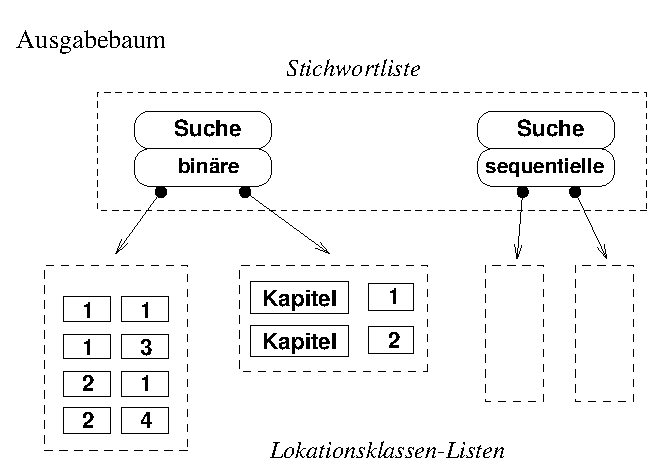
\epsfig{file=ausgabebaum.eps}

  \vspace*{5mm}

  \noindent \Hierzwei{Suche}{bin�re}: 1.1, 1.3, 2.1, 2.4; Kapitel 1,
  Kapitel 2, \ldots
\end{tfigure}

Bei der Ausgabeformatierung m�ssen wir nun den kompletten Baum
geeignet traversieren und entlang der Knoten und Verbindungen
entsprechende Zeichenketten in den Ausgabestrom schreiben. Die
Traversierung mu� auf die gew�nschte Ausgabeform anpa�bar sein.
Betrachten wir die Lokationen in der Abbildung, so sind \zB die
folgenden Ausgabeformen denkbar:
%
\begin{enumerate}
\item 1.1, 1.3, 2.1, 2.4; Kapitel 1, Kapitel 2
  \label{ausg:sequentiell}
\item \ldots{}; Kapitel 1, 2
  \label{ausg:bumper}
\item 1 \  1,3; 2 \ 1,4; \ldots
\end{enumerate}
%
Wir m�ssen demnach in der Lage sein, Strukturkomponenten
einzeln ausgeben zu k�nnen und zus"atzlich die Ausgabe von bestimmten
Elementen des Ausgabebaums gezielt zu unterdr�cken.

%%Wir teilen dazu die Ebenen einer Lokationsklasse in \emph{aktive} und
%%\emph{passive}\remark{aktive und passive Strukturkomponenten} ein. Ein
%%aktiver Knoten wird bei der Ausgabe nur einmal ausgegeben wie das Wort
%%\quasi{Kapitel} in Fallbeispiel~2 oder die oberste Strukturkomponente der
%%Gliederungsnummern in Fallbeispiel~3. Dagegen kann der Wert von
%%passiven Strukturkomponenten mehrfach ausgegeben werden wie in
%%Fallbeispiel~1.


%Wir m�ssen also f�r die Lokationsklasse der Kapitel den Baum in einer
%Hauptreihenfolge durchlaufen, w�hrend wir f�r die Lokationsklasse der
%Abschnittsnummern \Quasi{jojo--artig} durch den Baum auf und ab laufen
%m�ssen. Wir m�ssen also f�r alle Lokationsklassen die Traversierung
%separat festlegen, wobei wir im folgenden zwischen aktiven und
%passiven Knoten unterscheiden.

%\begin{Def}\mbox{}\par
%  \begin{circleitemize}
%  \item Ein \emph{aktiver} Knoten oder \emph{Bumper}\footnote{Dieser
%      Name soll die Vorstellung ausdr�cken, da� das gedachte JoJo an
%      dieser Stelle beim Hochlaufen gegen ein Hindernis st��t und
%      zur�ckgesto�en wird.} ist ein Knoten, der beim Traversieren
%    nicht nach oben verlassen werden darf, ohne da� alle Elemente des
%    Knotens inklusive ihrer Unterb�ume abgearbeitet wurden.
%  \item Ein \emph{passiver} Knoten kann w�hrend des Traversierens nach
%    oben verlassen werden.
%  \item Der oberste Knoten einer Lokationsklasse ist immer ein aktiver
%    Knoten.
%  \end{circleitemize}
%\end{Def}

%\noindent Betrachten wir nun die Beispiele der Abbildung, so sind f�r
%die Ausgabeform~\ref{ausg:sequentiell} die Knoten A$_1$ und B$_1$
%aktive Knoten, w�hrend f�r die Ausgabeform~\ref{ausg:bumper} auch noch
%der Knoten A$_{1,1}$\footnote{A$_{x,y}$ bezeichnet im Baum A den
%  Unterknoten $y$ des Unterknotens $x$ von A} aktiv ist. Ordnen wir
%nun an geeigneten Stellen Ausgabekommandos in die Traversierung ein,
%so sind wir prinzipiell in der Lage alle m�glichen Ausgabevarianten zu
%realisieren, die mit Hilfe dieser Traversierung durchf�hrbar sind.
\subsection{Traversierung des Ausgabebaums}
\label{sec:travAusgabebaum}

Nun stellt sich die Frage nach den notwendigen Ausgabekommandos und
dem Traversierungsalgorithmus. Folgende Ausgabekommandos sind anhand
der Traversierung und der Durchsicht verschiedener Indexe entworfen
worden:
%
\begin{circleitemize}

\item Beim erstmaligen Eintritt in einen Knoten und beim endg�ltigen
  Verlassen sollten Ausgabekommandos definierbar sein:
  \textsf{pre-print-node} und \textsf{post-print-node}.

\item Vor und nach einer Strukturkomponente: \textsf{pre-print-layer} und
  \textsf{post-print-layer}.

\item Die Strukturkomponente, also das Element selbst:
  \textsf{print-element}.

\item Bei listenf�rmigen Aufz�hlungen mit Trennzeichen ist es
  w�n"-schens"-wert, Trennzeichen \emph{nach} dem letzten Element
  unterdr�cken zu k�nnen. Wir bezeichnen das Ausgabekommando, welches
  immer nach einer Strukturkomponente, aber nicht nach der letzten
  Strukturkomponente ausgegeben wird, als
  \textsf{optional-post-print-layer}.

  Beispiel: 1.1, 1.3, 1.5$[,]$

\item Bei der Aufz�hlung von Bereichen (\zB 1.2--1.5) mu� das
  Bereichstrennzeichen (in diesem Fall \quasi{--}) definierbar sein.
  Es tritt beim Ausdruck von Bereichen an die Stelle von
  \textsf{optional-post-print-layer}. Wir bezeichnen es mit
  \textsf{optional-range}.

\item Es ist vor allem bei Stichw�rtern notwendig, ein
  Wiederholungssymbol definieren zu k�nnen. Oft findet man Indexe in
  der Form
  \begin{tabbing}
      \hspace{1cm}\=S\=uche\=, bin�re \hspace{3em} \=\ldots\\
                  \>\>$\widetilde{\ \ \ }$\>, sequentielle \>\ldots
  \end{tabbing}
  Hier wird das Tilde-Zeichen als Wiederholungssymbol f�r das
  Stichwort der ersten Ebene verwendet. �blicherweise wird das
  Wiederholungszeichen an jedem Seiten- oder Spaltenanfang nicht
  verwendet, um dem Leser eine leichtere Orientierung zu erm�glichen.
  Das Erkennen des Seitenanfangs oder anderer Positionen im Dokument
  kann jedoch nur durch das Textsatzsystem geleistet werden.  Dieses
  Wiederholungssymbol bezeichnen wir mit \textsf{repetition-symbol}.

\item Wir ordnen jedem Knoten die Eigenschaft \emph{aktiv} oder
  \emph{passiv} zu. Ein aktiver Knoten erzwingt bei der Ausgabe seine
  Einreihung in den momentanen Ausgabestrom. Ein passiver Knoten
  �berl��t die Entscheidung �ber seine Einreihung der
  Formatierungsroutine, die mittels Kontextvergleich die passende
  Einordnungsstrategie ermittelt.

\end{circleitemize}

\newcommand{\indexopen}[1]{\textit{#1}$_{\scriptscriptstyle(}$}
\newcommand{\indexclose}[1]{\textit{#1}$_{\scriptscriptstyle)}$}

\begin{ttable}%
  {Tabelle mit Ausgabematrizen f�r unterschiedliches Markup eines
    Ausgabebaums}%
  {tab:ausgabematrix}%
  \centering%
  \begin{tabular}{|c|c|c|c|c|c|c|c|c|}
    \hline%
    \multicolumn{9}{|c|}{\textbf{Ausgabematrix}\medrule}\\
    \hline\hline
    \multicolumn{9}{|c|}{\smallrule Ausgabeform:\, 1.1.1, 1.1.2,
      1.2.1--1.2.3, \ldots{} 2.1.1 \ldots{} $x.y.z$}\\
    \hline%
    \textit{Typ} & \textsf{pre-} &
    \textsf{pre-} & \textsf{layer} & \textsf{rep.-} & \textsf{post-} &
    \multicolumn{2}{|c|}{\textsf{optional-}} & \textsf{post-} \\[-2pt]
    & \textsf{node} & \textsf{layer} & & \textsf{symbol} & \textsf{layer} &
    \textsf{post-layer} & \textsf{range} & \textsf{node} \\
    \hline%
    \textsf{A}  & &                    & \textit{num} & & &
    \quasi{\textbf{,}$\sqcup$} & &\\
    \textsf{A} & & \quasi{\textbf{.}} & \textit{num} & & & & &\\
    \textsf{A} & & \quasi{\textbf{.}} & \textit{num} & & & &
    \quasi{\textbf{--}} &\\
    \hline%
    \hline%
    \multicolumn{9}{|c|}{\smallrule Ausgabeform:\, \textbf{1} 1.1, 1.2,
      2.1--2.3, \ldots{}; \textbf{2} $x.y$, \ldots{}}\\
    \hline%
    \textit{Typ} & \textsf{pre-} &
    \textsf{pre-} & \textsf{layer} & \textsf{rep.-} & \textsf{post-} &
    \multicolumn{2}{|c|}{\textsf{optional-}} & \textsf{post-} \\[-2pt]
    & \textsf{node} & \textsf{layer} & & \textsf{symbol} & \textsf{layer} &
    \textsf{post-layer} & \textsf{range} & \textsf{node} \\
    \hline%
    \textsf{P} & & {\small\slshape bold-on} & \textit{num} & &
    {\small\slshape bold-off} & \quasi{\textbf{;}$\sqcup$} & &\\
    \textsf{A} & \quasi{$\sqcup$} & & \textit{num} & & &
    \quasi{\textbf{,}$\sqcup$} & &\\
    \textsf{A} & & \quasi{\textbf{.}} & \textit{num} & & & &
    \quasi{\textbf{--}} &\\
    \hline
  \end{tabular}

  \smallskip

\end{ttable}


\noindent Daraus ergibt sich nun eine Definitionsmatrix, in der f�r jede
Strukturkomponente einer Lokationsklasse die Ausgabekommandos
definiert werden k�nnen und die Komponenten als aktive (\textsf{A})
oder passive Einheiten (\textsf{P}) festgelegt werden m�ssen. Eine
entsprechende Beispielmatrix ist in Tabelle~\ref{tab:ausgabematrix}
dargestellt.

Als nat�rliches Durchlaufverfahren des Ausgabebaums w�hlen wir eine
modifizierte Version der Traversierung \emph{Hauptreihenfolge}.

Jeder Ebene eines Stichworts und jeder Strukturkomponente einer
Lokationsklasse wird ein entsprechendes Markup zugewiesen. Bei der
Ausgabe eines neuen Stichworts wird als \emph{Kontext}\remark{Kontext}
der Druckschl�ssel des vorherigen Stichworts mitgegeben. Die
Formatierungsroutine kann durch einen Vergleich dieses Kontexts mit
dem aktuellen Stichwort entscheiden, ab welcher Ebene sich beide
unterscheiden. Passive Knoten werden bei Gleichheit mit dem Kontext
unterdr�ckt. Unterscheiden sich Kontext und Schl�ssel, oder ist das
Markup einer Ebene aktiv oder mit einem Wiederholungssymbol versehen,
wird die Ausgabe des Knotens gestartet.

Entscheidet sich die Formatierungsroutine f�r eine Ausgabe einer
Strukturkomponente, so werden die Formatierungsanweisungen f�r das �ffnen
von Umgebungen in den Ausgabestrom hineingeschrieben.

Die Formatierungsanweisungen zum Schlie�en der jeweiligen Umgebungen
werden auf einem Stapel\remark{Umgebungs\-stapel} abgelegt, da ihre
Ausgabe verz�gert werden mu�, bis die Unterstrukturen abgearbeitet
sind. Da sich die Stichw�rter und Lokationsreferenzen an bestimmten
Stellen in den Ausgabeproze� einreihen, mu� bei der Einreihung daf�r
gesorgt werden, da� der Stapel mit den Umgebungen immer geeignet
geleert wird und die Anweisungen in den Ausgabestrom eingef�gt werden.
Dies beschreibt ein einfaches aber m�chtiges Verfahren, die Ausgabe
von Lokationsreferenzen zu steuern.


%%Hierbei gibt ein passives Element seine Repr�sentation an seine Kinder
%%weiter, w�hrend ein aktiver Knoten eine leere Zeichenkette weitergibt.
%%Eine \emph{Repr�sentation} besteht aus der Komposition von
%%\textsf{pre-print-layer}, \textsf{print-element} und
%%\textsf{post-print-layer}. Ein aktiver Knoten f�gt seine
%%Repr�sentation selbst dem Ausgabestrom hinzu. Ansonsten sind die
%%Bl�tter des Ausgabebaums daf�r zust�ndig, die �bergebene
%%Repr�sentation ihrer Vorg�nger vor der Ausgabe der eigenen
%%Repr�sentation in den Ausgabestrom einzuleiten.


%Eine vereinfachte \LISP-�hnliche Notation dieses Algorithmus ist wie folgt:
%\begin{verbatim}
%(defun print-node (current-node prefix-of-father)
%  (let ((prefix nil))
%    (if (is-active current-node)
%        (progn
%          (do-write current-node)
%          (setq prefix ""))
%        (progn
%          (setq prefix
%                (append prefix-of-father
%                        do-return current-node))))
%    (dolist (son list-of-all-sons)
%      (print-node son))))
%\end{verbatim}

%Der resultierende Algorithmus ist f�r die
%aktionsgebundene Traversierung ist in
%Abbildung~\ref{alg:controlled-jojo-traverse} dargestellt.

%\begin{tfigure}
%  {Algorithmus \emph{controlled-jojo-traverse} f�r die Traversierung
%    des Ausgabebaumes}
%  {alg:controlled-jojo-traverse}
%  \small
%  \begin{algorithm}
%    \ENUM \F{node-type} : $\{$\F{bumper}, \F{passive}$\}$;\\
%    \ENUM \F{control-mode} : $\{$\F{callback}, \F{finished}$\}$;\\[6pt]
%    \FUNC \F{controlled-jojo-traverse}
%          $($ \F{r} : \F{node}, \F{modevec}$[\ ]$ : \F{node-type} $)$;\\
%    \VAR \F{positionvec}$[\ ]$ \= $\equiv [0]$;\\
%    \>   \F{curr-control} : \F{control-mode};\\[6pt]
%    \>\FUNC \F{inner-traverse} $( r : \F{node}, \F{lay} : \F{int}
%    )$ : \F{control-mode};\\
%    \>\VAR \F{position} $\equiv$ \F{positionvec}$[\F{lay}]$;\\
%    \>\BEGIN\\
%    \>\>\IF (\F{position} $=$ 0) \THEN \ACTION{\textsf{pre-print-node}};\\
%    \>\>\REPEAT \texttt{//} {\small\slshape Schleife �ber alle Elemente eines Kontens}\\
%%    \>\>\>\IF (\F{position} $>$ 0) \THEN
%%    \ACTION{\textsf{optional-pre-print-layer}};\\
%    \>\>\>\F{position} $\equiv$ \F{position}$+ 1$;\\
%    \>\>\>\REPEAT \texttt{//} {\small\slshape Schleife �ber alle Callbacks
%      eines Knotens}\\
%    \>\>\>\>\ACTION{\textsf{pre-print-layer}};\\
%    \>\>\>\>\ACTION{\textsf{print-layer}};\\
%    \>\>\>\>\F{curr-control} $\equiv$
%             \F{inner-traverse}(\F{r}$[\F{position}]$ , \F{lay}$+ 1$);\\
%    \>\>\>\>\ACTION{\textsf{post-print-layer}};\\
%    \>\>\>\>\texttt{//} {\small\slshape Beende Schleife falls passiver Knoten
%      oder Subknoten fertig}\\
%    \>\>\>\UNTIL( \=( \=(\F{modevec}$[\F{lay}]$ $=$ \F{bumper}) \AND\\
%    \>\>\>        \>  \>(\F{curr-control} $=$ \F{finished}) ) \OR\\
%    \>\>\>        \>(\F{modevec}$[\F{lay}]$ $=$ \F{passive}) )\\
%    \>\>\>\IF (\F{curr-control} $=$ \F{finished}) \THEN\\
%    \>\>\>\>\F{position} $\equiv \F{position} + 1$;\\
%    \>\>\>\IF (\F{position} $<$ \F{maxelement}($r$)) \THEN\\
%    \>\>\>\>  \ACTION{\textsf{optional-post-print-layer}};\\
%    \>\>\>\texttt{//} {\small\slshape Beende Schleife falls passiver Knoten
%      oder alle Elemente bearbeitet}\\
%    \>\>\UNTIL( \=(\F{modevec}$[\F{lay}]$ $=$ \F{passive}) \OR\\
%    \>\>     \>( \=(\F{modevec}$[\F{lay}]$ $=$ \F{bumper}) \AND\\
%    \>\>     \> \>(\F{position} $>$ \F{r}$[$\F{maxelement}(\F{r})$]$) ) )\\
%    \>\>\F{positionvec}$[\F{lay}]$ $\equiv$ \F{position};\\
%    \>\>\IF (\EXPR{Range follows}) \THEN
%      \ACTION{\textsf{optional-print-range}}; \ENDIF\\
%    \>\>\IF (\F{position} $\ge$ \F{r}$[$\F{maxelement}(\F{r})$]$) \THEN\\
%    \>\>\>\ACTION{\textsf{post-print-node}};\\
%    \>\>\>\RETURN (\F{finished});\\
%    \>\>\ELSE\\
%    \>\>\>\RETURN (\F{callback});\\
%    \>\>\ENDIF\\
%    \>\ENDFUNC\\[6pt]
%    \BEGIN\\
%    \>\F{inner-traverse}($r$, 1);\\
%    \ENDFUNC
%  \end{algorithm}
%\end{tfigure}


\subsection{Stichwortgruppen}

Bei der Darstellung von Indexen ist es �blich,
Stichwortgruppen\remark{Stichwortgruppen} durch spezielle
Informationen visuell darzustellen. Oft bildet man Stichwortgruppen
nach dem ersten Buchstaben eines Stichworts und trennt beispielsweise
in einem Index jede Buchstabengruppe optisch voneinander ab. Da eine
solche optische Abtrennung Teil der Ausgabeformatierung ist, m�ssen
wir auf geeignete Weise die Definition von Stichwortgruppen und deren
Markup vorsehen.

Da die Sortierung der
Stichw�rter bereits durch das sort-mapping festgelegt wurde, m�ssen wir
uns einfach nur eine Liste von Stichwortgruppen durch Tupel der Form
\begin{center}
  \lettergrp $= ( \keyword, \markup )$\, mit\, \keyword, \markup\ :
  \textsl{String}
\end{center}
definieren und k�nnen beim Traversieren des Stichwortbaums bei
�ber\-schrei\-ten der Gruppengrenzen die entsprechenden Markups in den
Ausgabestrom einf�gen. Im \textsf{makeindex}-System von
\cite{Chen:SPE-19-9-897} werden Stichwortgruppen grund\-s�tz\-lich nur
aus den Anfangsbuchstaben der Stichw�rter gebildet und optische
Trennungen in den Ausgabestrom eingef�gt. Im \emph{International
  MakeIndex} \cite{Schrod:CG-10-81} werden Anweisungen eingef�hrt,
welche die Bildung von zus�tzlichen Buchstabengruppen und deren Markup
erlaubt.

Die in diesem Verfahren angewandte Grundidee besteht aus einem
zus�tzlichen Mapping des Sortierungsschl�ssels eines Indexeintrags auf
einen \emph{Stichwortgruppenschl�ssel}. Dieses Mapping wird in den
Systemen implizit als die Abbildung auf den ersten Buchstaben
angenommen.

Wir erweitern die Ausgabe zu einem zweischichtigen Modell durch die
Bildung von Stichwortgruppen, denen jeweils ein zus�tzliches Markup
zugeordnet wird. Wir beschreiben die Ausgabeinformationen in einer
Liste $G$ von Stichwortgruppen mit $G = \{g_1,\ldots{},g_n\}$ mit $g_i
= (\{l_1,\ldots{},\l_m\}, \markup)$.  Die Elemente $g_i$ sind also
Obergruppen, denen als Gesamtheit ein Markup zugeordnet ist, w�hrend
die $l_i$ Stichwortgruppen der �blichen Form sind. Ein Markup besteht
in der einfachsten Form aus einem Paar von Strings, welche die
entsprechenden Formatierungs-Umgebungen einleiten und abschlie�en.

Diese Definition erscheint uns im Moment ausreichend genug, um auch
komplexere Indexe geeignet auszugeben.


\section{Indexstyle}

Mit dem Abschlu� des vorigen Abschnitts haben wir nun die
grundlegenden Parameter des Indexsystems umrissen. Dies gibt uns nun
die M�glichkeit, das Datenmodell des
\emph{Indexstyles}\remark{Indexstyle} zu entwerfen. Der Indexstyle ist
die Zusammenfassung aller Parameter und Spezifikationen, mit denen
unser System in der Lage sein soll, einen Indexierungsproze�
durchzuf�hren. Zu diesen Parametern z�hlen \ua die folgenden Daten:

\begin{circleitemize}

%\item Spezifikation des Eingabeformates der Rohdaten.

\item Beschreibung der Lokationsklassen mit Struktur und Regelwerk.

\item Beschreibung der Indexklassen, insbesondere deren
  Ausgabeformatierung.

\item Regelwerk zum Mischen und Sortieren der Stichw�rter.
  Insbesondere das regelbasierte Substitutionsschema analog zum
  \emph{International MakeIndex}.

\item Informationen zur Ausgabeformatierung des kompletten Indexes mit
  der Definition von Stichwortgruppen.

\end{circleitemize}

\noindent Aus der Menge der Parameter wird auch das Ziel der Arbeit
deutlich, ein hoch parametrisierbares und individuell vom Benutzer
definierbares Indexsystem zu entwerfen. M�glichst viele Parameter
sollen in die externe Spezifikation ausgelagert werden, um h�chste
Konfigurierbarkeit zu erlangen.

Bei den folgenden Definitionen verwenden wir bei Bezeichnern den
Exponenten \isindex{}{}, um kenntlich zu machen, da� es sich um
Datenelemente des Indexstyles handelt. Weil wir hier die Parameter von
realen Objekten des Indexeintrags beschreiben, bietet es sich an,
�hnliche Bezeichner daf�r zu verwenden, um die Analogie kenntlich zu
machen. Gleichzeitig schlie�en wir eine Verwechslung mit den Elementen
des Indexeintrags aus, die ohne Exponenten geschrieben werden.

%Im wesentlichen handelt es sich bei der Elementen im Indexstyle um die
%Parameter einer Objektklasse\footnote{vergleichbar mit statischen
%  Klassendaten in \cpp}, w�hrend entsprechende Elemente im
%Indexeintrag instanziierte reale Objekte handelt.

\begin{Def}
  Ein \textbf{Indexstyle} \idxstyle ist eine Liste von Indexklassen
  \begin{center}
    \idxstyle $= ($ \isidxclsSet $)$ .
  \end{center}
\end{Def}

\begin{Def}
  Eine \textbf{Indexklasse} \isidxcls ist ein Tupel
  \begin{center}
    \isidxcls $=$ $($ \isidxclsname, \isbasetypeSet, \ismapruleSet,
    \isidxtagSet $)$
  \end{center}
  mit den Komponenten
  \begin{deflistcolon}{\isidxclsname}
  \item[\isidxclsname] \textbf{Klassenname}, String
  \item[\isbasetypeSet] \textbf{Komponententypen}, Alphabete und Aufz�hlungen
  \item[\islocclsSet]  \textbf{Lokationsklassen}
  \item[\isidxtagSet]  \textbf{Markup-Informationen}.
  \end{deflistcolon}
\end{Def}

%%\begin{Def}
%%  Eine \textbf{Abbildungsregel} \ismaprule ist ein Tupel
%%  \begin{center}
%%    \ismaprule $=$ $($ \isruletype, \ispattern, \isreplace $)$
%%  \end{center}
%%  mit den Komponenten
%%  \begin{deflistcolon}{isruletype}
%%  \item[\isruletype] \textbf{Regeltyp}, Element aus \isruletypes $=
%%    \{${\normalfont \textsf{sort}, \textsf{merge}}$\}$.
%%  \item[\ispattern]  \textbf{Regul�rer Ausdruck}, String
%%  \item[\isreplace]  \textbf{Regul�rer Ausdruck}, String
%%  \end{deflistcolon}
%%\end{Def}


\begin{Def}
  Eine \textbf{Lokationsklasse} \isloccls ist ein Tupel
  \begin{center}
    \isloccls $= ($ \islocclsname, \islaystruc, \islocrefruleSet $)$
  \end{center}
  mit den Komponenten
  \begin{deflistcolon}{\islocclsname}
  \item[\islocclsname]   \textbf{Lokationsklassenname}, String
  \item[\islaystrucSet]  Menge der \textbf{Lokationsstrukturkomponenten}
  \item[\islocrefruleSet]Menge der
    \textbf{Lokationsverarbeitungsregeln}, siehe
    Definition~\ref{def:lokationsverarbeitungsregel} auf
    Seite~\pageref{def:lokationsverarbeitungsregel}.
  \end{deflistcolon}
\end{Def}

\begin{Def}
  Eine \textbf{Lokationsstrukturkomponente} \islaystruc ist ein Tupel
  \begin{center}
    \islaystruc $= ($ \isbasetype, \issep $)$
  \end{center}
  mit den Komponenten
  \begin{deflistcolon}{\issep}
  \item[\isbasetype] \textbf{Komponententyp}, Element aus \isbasetypes
    %$= \{${\normalfont\textsf{num}, \textsf{alpha},
    %  \textsf{Alpha}, \textsf{roman}, \textsf{Roman},
    %  \textsf{userdefined}}$\}$
  \item[\issep] \textbf{Trennzeichen}, String.
  \end{deflistcolon}
\end{Def}

\noindent Mit diesen Definitionen haben wir das schematische
Datenmodell des Indexstyles festgelegt. Wir verzichten auf eine
detailliertere Beschreibung aller Komponenten, da sie f�r das
Verst�ndnis des Gesamtsystems nicht relevant sind.

Um die Benutzbarkeit des Systems zu erh�hen, definieren wir eine
\texttt{default}-Indexklasse, deren Definitionen in allen anderen
Indexklassen ebenfalls gelten sollen. Die Festlegungen dieser
Indexklasse werden jedoch von Definitionen in den jeweiligen Klassen
�berschrieben.


%%Die fehlenden Definitionen f�r die Darstellung der Grammatik des
%%Eingabeformates wird nicht modelliert, da wir prinzipiell nur an der
%%Grammatik selbst und nicht an ihrer Darstellung interessiert sind.

%%Wie im Datenmodell des Indexeintrags geben wir hier ebenfalls eine
%%grobe hierarchische �bersicht in Abbildung~\ref{fig:indexstyle}.

%%\begin{tfigure}%
%%  {�berblick �ber das Datenmodell einer Indexklassenbeschreibung in
%%    hierarchischer Darstellung}%
%%  {fig:indexstyle}%
%%  \begin{tabbing}
%%    \hspace*{0.5cm} \=
%%    \hspace*{0.5cm} \=
%%    \hspace*{0.5cm} \=
%%    \hspace*{0.5cm} \=
%%    \hspace*{0.5cm} \=
%%    \hspace*{0.5cm} \=
%%    \hspace*{2.5cm} \=
%%    \kill
%%    \idxstyle\\
%%    \> \isidxclsSet\\
%%    \> \> \isidxcls $[1]$\\
%%    \> \> \> \isidxclsname  \> \> \> \> \quasi{Autor}\\
%%    \> \> \> \ismapruleSet\\
%%    \> \> \> \> \ismaprule $[1]$\\
%%    \> \> \> \> \> \isruletype \> \> \textsf{sort}\\
%%    \> \> \> \> \> \ispattern  \> \> \verb|"\"A"|\\
%%    \> \> \> \> \> \isreplace  \> \> \verb|"ae"|\\
%%    \> \> \> \> \ismaprule $[2]$\\
%%    \> \> \> \> \> \isruletype \> \> \textsf{merge}\\
%%    \> \> \> \> \> \ispattern  \> \> \verb|"\\?\"[AaOoUus]"|\\
%%    \> \> \> \> \> \isreplace  \> \> \verb|"&"|\\
%%    \> \> \> \isidxtagSet\\
%%    \> \> \isidxcls $[2]$\\
%%    \> \> \> \isidxclsname  \> \> \> \> \quasi{Gesamt}\\
%%    \> \> \> \ldots\\
%%    \> \> \isidxcls $[3]$\\
%%    \> \> \> \isidxclsname  \> \> \> \> \quasi{Kommandos}\\
%%    \> \> \> \ismapruleSet\\
%%    \> \> \> \> \ismaprule $[1]$\\
%%    \> \> \> \> \> \isruletype \> \> \textsf{sort}\\
%%    \> \> \> \> \> \ispattern  \> \> \verb|"^\(.*)"|\\
%%    \> \> \> \> \> \isreplace  \> \> \verb|"\1"|\\
%%    \> \> \> \> \ldots\\
%%    \> \> \> \isidxtagSet\\
%%    \> \> \> \> \ldots\\
%%    \> \islocclsSet\\
%%    \> \> \isloccls $[1]$\\
%%    \> \> \> \islocclsname  \> \> \> \> \quasi{LaTeX-Section}\\
%%    \> \> \> \islaystrucSet \> \> \> \> \Strukdrei{num}{.}{num}{.}{num}\\\
%%    \> \> \> \isloclsortorderSet \> \> \> \> $\{$\textsf{default},
%%    \textsf{bold}, \textsf{italic} $\}$  \\
%%    \> \> \> \islocrefruleSet \> \> \> \> \ldots\\
%%    \> \> \ldots\\
%%    \> \isidxgram\\
%%    \> \> \ldots%
%%  \end{tabbing}%
%%%
%%% Beispiel:
%%% \begin{tabbing}
%%%   Lokationsreferenzen \= \kill
%%%   Stichwort           \>: \Hierzwei{Suche}{bin�re}\\
%%%   Lokationsreferenz   \>: \textbf{2.1}\textit{f.}\\
%%%   Lokationsklasse     \>: \quasi{Gesamtindex}\\
%%% \end{tabbing}%
%%\end{tfigure}



%% Local Variables:
%% mode: latex
%% TeX-master: "makeindex4.tex"
%% TeX-master: t
%% End:

%%
%% $Log$
%% Revision 1.5  1995/11/15 14:58:12  kehr
%% Final correction (I hope so).
%%
%% Revision 1.4  1995/11/14  16:05:57  kehr
%% Made two more corrections on the report.
%%
%% Revision 1.3  1995/11/08  16:17:01  kehr
%% New correction.
%%
%% Revision 1.2  1995/10/20  11:57:35  kehr
%% Korrektur nach Klaus' Durchsicht.
%%
%% Revision 1.1  1995/10/16  17:31:53  kehr
%% Initial checkin of Report and Presentation.
%%
%% Revision 1.26  1995/10/06  23:05:16  kehr
%% Korrektur nach der Durchsicht von Karin.
%%
%% Revision 1.25  1995/09/22  01:12:07  kehr
%% Zweite �berarbeitung nch der inhaltlichen Korrektur. Au�erdem habe
%% ich das Logo zu MacIndex ver�ndert. Hat jetzt mehr pepp !
%%
%% Revision 1.24  1995/09/21  00:05:45  kehr
%% Erste Ver�nderungen nach der inhaltlichen Korrektur durch Joachim am
%% 20.Sep.95. Fast alle Dateien d'sind davon betroffen. Au�erdem sind noch zwei
%% neue Abbildungen hinzugekommen.
%%
%% Revision 1.23  1995/09/06  18:52:51  kehr
%% Made final changes before giving for correction.
%%
%% Revision 1.22  1995/08/28  18:08:17  kehr
%% Neue Einspielung der xfig-Dateien
%%
%% Revision 1.21  1995/07/04  09:46:30  kehr
%% Weitere �nderungen. Bin aber fast fertig.
%%
%% Revision 1.20  1995/07/04  00:46:52  kehr
%% Bald ist's soweit ;-)
%% Ich habe heute die generelle Umstrukturierung vorgenommen und einige
%% Teile herausgeschmissen. Die Indexverarbeitung mu� noch �berarbeitet werden.
%%
%% Revision 1.19  1995/06/18  23:32:24  kehr
%% Schlu� f�r heute. Genug geschafft.
%%
%% Revision 1.18  1995/06/18  19:10:38  kehr
%% Lokationsverarbeitung geblickt !;-)
%%
%% Revision 1.17  1995/06/17  20:36:30  kehr
%% Habe die Lokationsreferenzverarbeitung umstrukturiert und besser
%% definiert. DIe Buchstabengruppen m�ssen noch beendet werden und der
%% Algorithmus zum Mischen und Sortieren der Lokationsreferenzen mu�
%% fertiggestellt werden.
%%
%% Revision 1.16  1995/06/15  12:58:43  kehr
%% Erweiterung der Ausgabematrix und kleinere �nderungen am Layot.
%% �berpr�fe jetzt das ganze Dokument, um mich auf die beiden letzten
%% Probleme einzulesen.
%%
%% Revision 1.15  1995/06/13  21:55:16  kehr
%% Habe heute die Formulierung des Algorithmus controlled-jojo-traverse
%% fertiggestellt. Desweiteren Fehler in der Anwendung der \lindent-Umgebung
%% gefunden. Ich mu� noch die Matrix f�r die Definition der Ausgabekommandos
%% und der Angabe im Indexstyle entwickeln.
%%
%% Revision 1.14  1995/06/09  20:59:51  kehr
%% Superviel gemacht heute ;-)
%%
%% Revision 1.13  1995/06/08  20:19:48  kehr
%% Bibliographie erweitert.
%%
%% Revision 1.12  1995/06/08  11:25:59  kehr
%% Implementierungsteil angefangen.
%%
%% Revision 1.11  1995/06/08  00:35:54  kehr
%% Was soll ich blo� schreiben ???
%%
%% Revision 1.10  1995/06/07  20:59:13  kehr
%% Und weiter am Modellentwurf. Spezifikation des Indexstyles vorerst
%% fertig. Es fehlt noch die Eingabegrammatik.
%%
%% Revision 1.9  1995/06/07  11:24:21  kehr
%% Definitionen der Indexstyle-Elemente.
%%
%% Revision 1.8  1995/06/06  23:50:14  kehr
%% Modellentwurf weitergebracht.
%%
%% Revision 1.7  1995/06/06  17:51:02  kehr
%% Commit um die �nderungen festzuhalten.
%%
%% Revision 1.6  1995/06/06  11:50:35  kehr
%% Weitere Bearbeitung des Modellentwurfs.
%%
%% Revision 1.5  1995/05/31  19:18:52  kehr
%% Fertigstellung des Analyse-Abschnitts (Hoffentlich ;-).
%%
%% Revision 1.4  1995/05/28  21:37:11  kehr
%% Neue �berarbeitete Version.
%% Inhaltliche �nderungen:
%%   Glossar hinzugenommen. Einleitung mit Datenflu�graph. Kleinere
%%   �nderungen an der Beschreibung des International Makeindex.
%% System�nderungen:
%%   Makefile-�nderungen, Stil�nderungen, Titelseite
%%
%% Revision 1.3  1995/05/05  23:07:15  kehr
%% Ge�nderte Datenstrukturen mit enumerate und neuen labels f�r enumerate
%%
%% Revision 1.2  1995/05/05  22:25:05  kehr
%% Ge�nderte Struktur mit einleitung.tex
%% Zwischenspeicherung vor der Umstellung der Definnitionen
%%
%% Revision 1.1  1995/04/28  22:15:26  kehr
%% Weitere Dateien eingecheckt.
%%
%%


%%% Local Variables:
%%% mode: latex
%%% TeX-master: t
%%% End:


%%
%% $Id$
%%
%% Document: Indexverarbeitung `makeindex4' - Projekt
%%

\chapter{Indexverarbeitung}
\label{sec:indexverarbeitung}

Wir kommen nach der Daten- und Strukturmodellierung in
Abschnitt~\ref{sec:modellentwurf} zu den einzelnen Verfahren der
Indexverarbeitung. Vergegenw�rtigen wir uns dazu noch die Einbettung
des Indexierungssystems in den Proze� der Indexerstellung, wie er in
Abbildung~\ref{fig:datenfluss} auf Seite~\pageref{fig:datenfluss}
dargestellt ist.

Wir betrachten nun die einzelnen Abschnitte der Indexverarbeitung und
behandeln insbesondere die Verarbeitung der Lokationsreferenzen
vertieft, weil sie im Hinblick auf die bestehenden Systeme neu
entwickelt wurde.

%Wir verwenden dazu formale Beschreibungen und eine pascal-�hnliche,
%algorithmische Notation.\footnote{Diese Algorithmen sollen das
%  grunds�tzliche Verfahren aufzeigen und sind in der tats�chlichen
%  Implementierung teilweise anders gel�st.}


\section{Indexstyle einlesen}

Das Einlesen des Indexstyles dient dazu, dem System alle Parameter
bekannt zu machen, die von Benutzerseite spezifiziert wurden. Der
Indexstyle ist eine Menge von Dateien, in denen in deklarativer Form
die Angaben �ber die Parameter des Indexsystems spezifiziert sind.
Diese Spezifikationen werden eingelesen und geeignet abgelegt.


\section{Indexeintr�ge einlesen und normalisieren}

%Durch das Einlesen des Indexstyles sind auch Informationen eingelesen
%worden, sie das Format der Datei beschreibt, welche die Rohindexdaten
%enth�lt. Anhand dieser Beschreibung werden die Indexeintr�ge
%und deren Komponenten eingelesen.

Die Indexeintr�ge werden eingelesen und jeweils ein internes Objekt
\idxent erzeugt. Dabei fallen noch die folgenden Aufgaben an:
%
\begin{circleitemize}
%\item Filterung aller Eintr�ge der Indexklasse die bearbeitet werden soll.
\item Der Indexeintrag mu� auf G�ltigkeit �berpr�ft werden.
\item Die Indexschl�ssel m�ssen durch die Sortier- und Mischregeln
  gegebenenfalls normalisiert werden.
\item Dem Indexeintrag mu� die passende Lokationsklasse zugeordnet werden.
\item Die Ordnungsnummern der einzelnen Strukturkomponenten m�ssen anhand
  der Lokationsklassendefinition errechnet werden.
\end{circleitemize}
%
Das \emph{Normalisieren}\remark{Normalisieren} der Indexschl�ssel wird
analog zum Verfahren des \emph{International Makeindex} durchgef�hrt.
Aus dem Schl�ssel \keyK wird mit den Mischregeln der Mischschl�ssel
gebildet, aus welchem mit Hilfe der Sortierregeln der Sortierschl�ssel
generiert wird.

%Das \textit{Normalisieren} der Indexschl�ssel wird nach dem Schema des
%\textit{International MakeIndex} vorgenommen, wo aus dem
%Indexschl�ssel \keyK der Indexschl�ssel \keyM mit Hilfe der
%Abbildungsregeln \ismapruleSet vorgenommen wird. Eine
%Regel\remark{Regel} ist eine Abbildung $\phi : \emph{Stichwort\/} \to
%\emph{Stichwort\/}$ und wird durch die Anwendung von regul�ren
%Ausdr�cken auf ein Stichwort. Wir betrachten die Mengen der Misch-
%und Sortierregeln, die wir folgt definiert sind:
%%
%\[ {\cal M} = \{ r \in \ismapruleSet\ \mid\ r.\isruletype =
%\textsf{merge} \}.\]
%%
%Analog definieren wir
%%
%\[ {\cal S} = \{ r \in \ismapruleSet\ \mid\ r.\isruletype =
%\textsf{sort} \}.\]
%%
%Fassen wir das Applizieren dieser Regeln als Funktionen auf, so gilt
%allgemein f�r die Normalisierung eines Schl�ssels $k$ durch eine
%Regelmenge ${\cal R}$:

%\begin{algorithm}
%  \FUNC \F{apply}( $k, {\cal R}$ )\\
%  \BEGIN\\
%  \>\FORALL $ r \in {\cal R} $ \DO \\
%  \>\> \textit{subst}( $r$, $k$ ) \\
%  \>\ENDDO\\
%  \ENDFUNC
%\end{algorithm}


%\noindent Die Funktion \F{subst}() wendet die Regul�ren
%Ausdr�cke $r$.\ispattern und $r$.\isreplace auf den Schl�ssel $k$ an.
%Wir k�nnen jetzt den kompletten Normalisierungsproze� algorithmisch
%beschreiben:

%\begin{algorithm}
%  \FUNC \F{normalize}( \VAR $i :$ \idxent )\\
%  \BEGIN\\
%  \>\IF \F{empty}($i$.\keyM) \THEN\\
%  \>\> $i$.\keyM $\equiv$ $i$.\keyK\\
%  \>\> \F{apply}( $i$.\keyM, ${\cal M}$ )\\
%  \>\ENDIF\\
%  \>$i$.\keyS $\equiv$ $i$.\keyM\\
%  \>\F{apply}( $i$.\keyS, ${\cal S}$ )\\
%  \ENDFUNC\\
%\end{algorithm}


\section{Stichwortmischung und -sortierung}
\label{sec:stwmischung}

Stichwortmischung dient dazu, alle Indexeintr�ge zusammenzufassen,
deren Mischschl�ssel \keyM identisch ist. Wir definieren dazu eine
Funktion \textit{join}, die zwei Indexeintr�ge miteinander vereinigt.

\newcommand{\Ione}{\mbox{${\cal I}_1$}}
\newcommand{\Itwo}{\mbox{${\cal I}_2$}}
\newcommand{\joinsymbol}{\mbox{$\triangleleft$}\xspace}

Diese Funktion kann folgenderma�en beschrieben werden. Seien \Ione{}
und~\Itwo{} Indexeintr�ge, so ist
\[\begin{array}{rl}
  \mbox{\textit{join}}(\Ione,\Itwo) \equiv (&\Ione.\keyK\ \joinsymbol\
  \Itwo.\keyK,\ \Ione.\keyM,\\
  & \Ione.\keyS\ \joinsymbol\ \Itwo.\keyS,\ \Ione.\keyP\ \joinsymbol\
  \Itwo.\keyP,\ \\ & \Ione.\locrefSet\ \cup\
  \Itwo.\locrefSet ).
\end{array}\]

\noindent Die Funktion \joinsymbol ist hier wie folgt definiert:
%
\[ x\ \joinsymbol\ y = \left\{
  \begin{array}{ll}
    y & \textrm{falls}\ x\ \textrm{leer}\\ x & \textrm{sonst} .
  \end{array}
\right.\]

\noindent Nach dem Mischen der zusammengeh�renden Indexeintr�ge wird der Index
lexikographisch anhand der Sortierschl�ssel sortiert.


%Folgende Beschreibung verdeutlicht dies:
%\begin{algorithm}
%  \FUNC \F{sortindex} ( \VAR \F{idx} : \indeX )\\
%  \BEGIN\\[6pt]
%  \>\FUNC \F{compare} ( \F{i,j} : \idxent ) : int\\
%  \>\BEGIN\\
%  \>\> return ( $i$.\keyS $\leq$ $j$.\keyS )\\
%  \>\ENDFUNC\\[6pt]
%  \>\F{sort} ( \textit{idx, compare} )\\
%  \ENDFUNC\\
%\end{algorithm}
%\noindent Hinter der Funktion \F{sort} kann sich eine geeignete
%Sortierroutine wie \zB \textit{Quicksort} verbergen.


\section{Lokationsreferenzmischung und -sortierung}
\label{sec:locrefmischung}

Durch die Hinzunahme von verschiedenen Lokationsklassen mu� die
Mischung und Sortierung von Lokationsreferenzen anhand der in
Abschnitt~\ref{sec:lokationsverarbeitung:regeln} definierten Misch-
und Sortierregeln erfolgen. Der Verarbeitungsproze� der
Lokationsreferenzen eines Indexeintrags gliedert sich in die folgenden
Phasen:

\begin{enumerate}
\item Lokationsklassenmatrix (\emph{siehe
    Abbildung~\ref{tab:Lokationsreferenzmatrix:eins}}) aufstellen. Den
  Lokationsreferenzen wird ihre Lokationsklasse zugeordnet. Die
  Kategorieattribute werden bei diesem Klassifizierungsproze� noch
  nicht beachtet.

\item Auf"|l�sen der Matrix und Mischen und Sortieren jeder einzelnen
  Lokationsklasse gem�� ihrer Kategorieattribute. Dieser Proze� l�uft
  in folgender Weise ab:

  \begin{enumerate}
  \item Unterteilung der Lokationsreferenzen in Mengen, deren Elemente
    zu einer Lokationsklasse geh�ren.

  \item Die gebildeten Lokationsreferenzmengen werden gem�� der
    Unterscheidung in Separate- und Mixedsorting bez�glich ihrer
    Kategorieattribute unterteilt.

  \item Aufl�sen der \textsf{merge-to}-Regeln, indem die
    entsprechenden Referenzen zus�tzlich in die Referenzmengen der
    Kategorie-Nachbarn eingef�gt werden (Prim�rattribut), wobei ein
    Hinweis auf ihr originales Kategorieattribut beibehalten wird
    (Sekund�rattribut).

  \item Sortieren dieser Mengen gem�� der definierten Totalen Ordnung.

  \item Erzeugung von Bereichen durch das Zusammenfassen von
    aufeinander folgenden Lokationsreferenzen. Dabei werden sowohl das
    Prim�rattribut als auch die Sekund�rattribute verwendet.

  \item Verdr�ngung von Lokationsreferenzen innerhalb von virtuellen
    Attributen durch Referenzen mit h�herer Vorrangstufe.

  \item Eliminierung von Lokationsreferenzen, welche durch eine
    \textsf{merge-to}-Regel nicht in einem Bereich aufgenommen werden
    konnten oder die aufgrund einer erfolgreichen
    \textsf{drop-if-merged}-Regel wegfallen. Des weiteren Eliminierung
    von Lokationsreferenzen aufgrund der \textsf{substitite}-Regel.

  \end{enumerate}

\end{enumerate}

\noindent Nach diesem Arbeitsabschnitt ist die grunds�tzliche Arbeit
am Index vollendet. Wir m�ssen uns zum Abschlu� mit der Ausgabe des
kompletten Indexes in den Ausgabestrom befassen.

\section{Ausgabeformatierung}

Die Ausgabe des Indexes ist im wesentlichen die in
Abschnitt~\ref{sec:ausgabe-tagging} beschriebene Traversierung des
Ausgabebaums. Wir m�ssen dem Ausgabestrom noch zus�tzliche
Informationen beif�gen, die im Indexstyle definiert sind. Desweiteren
m�ssen die Stichwortgruppen w�hrend der Traversierung korrekt erkannt
und die entsprechenden Ausgabekommandos aufgerufen werden.

%%Da sich aber prinzipiell das hier verwendete Verfahren mit Ausnahme
%%des Ausgabebaums nicht vom \textsf{makeindex}- und
%%\emph{International MakeIndex} unterscheidet, werden wir hier keine
%%besonderen Beschreibungen dieses Prozesses beif�gen.


%% Local Variables:
%% mode: latex
%% TeX-master: "makeindex4.tex"
%% End:

%%
%% $Log$
%% Revision 1.2  1995/10/20 11:57:34  kehr
%% Korrektur nach Klaus' Durchsicht.
%%
%% Revision 1.1  1995/10/16  17:31:53  kehr
%% Initial checkin of Report and Presentation.
%%
%% Revision 1.8  1995/10/06  23:05:14  kehr
%% Korrektur nach der Durchsicht von Karin.
%%
%% Revision 1.7  1995/09/22  01:12:04  kehr
%% Zweite �berarbeitung nch der inhaltlichen Korrektur. Au�erdem habe
%% ich das Logo zu MacIndex ver�ndert. Hat jetzt mehr pepp !
%%
%% Revision 1.6  1995/09/21  00:05:44  kehr
%% Erste Ver�nderungen nach der inhaltlichen Korrektur durch Joachim am
%% 20.Sep.95. Fast alle Dateien d'sind davon betroffen. Au�erdem sind noch zwei
%% neue Abbildungen hinzugekommen.
%%
%% Revision 1.5  1995/09/06  18:52:50  kehr
%% Made final changes before giving for correction.
%%
%% Revision 1.4  1995/08/28  18:08:15  kehr
%% Neue Einspielung der xfig-Dateien
%%
%% Revision 1.3  1995/07/04  09:46:29  kehr
%% Weitere �nderungen. Bin aber fast fertig.
%%
%% Revision 1.2  1995/06/18  23:32:23  kehr
%% Schlu� f�r heute. Genug geschafft.
%%
%% Revision 1.1  1995/06/18  22:50:20  kehr
%% HuHu. habe das cvs add die ganze Zeit vergessen...
%%
%%



%%
%% $Id$
%%
%% Document: Implementierung des `makeindex4' - Projekts
%%


\chapter{Implementierung}
\label{sec:implementierung}


In diesem Abschnitt soll auf die konkrete Implementierung des
\mkxvier-Systems eingegangen werden. Dabei wird kurz auf die
verwendete Programmiersprache und auf die Entwicklungsumgebung
eingegangen. Allgemeine Anforderungen an das System waren:
%
\begin{enumerate}
\item Das System sollte m�glichst portabel sein. Die bestehenden
  Indexsysteme werden besonders intensiv im Zusammenhang mit dem
  \TeX-\cite{texbook} \bzw{} \LaTeX-System~\cite{latex} genutzt. Es
  sollte m�glich sein, das zu entwickelnde System weiterhin in diesem
  Bereich einzusetzen, wenngleich das System auf andere
  Anwendungssysteme hin konfigurierbar ist.
\item Das System sollte eine einfache und schnelle Umsetzung des
  entworfenen Datenmodells in eine Programmiersprache erm�glichen und
  leicht erweiterbar sein.
  \label{forderung:datenmodell}
\item Es sollte eine m�glichst schnelle Implementierung gestatten und
  die wesentlichen Punkte des Modells umfassen. Zur Realisierung
  sollten auch fertige Bibliotheken verwendet werden.
  \label{forderung:entwicklungszeit}
\end{enumerate}
%

\section{Entwicklungsumgebung}

Aus den aufgef�hrten Forderungen haben wir uns zun�chst f�r die
Programmiersprache \cpp entschieden, da eine einfache Abbildung in
entsprechende Klassen m�glich ist. Diese Sprache ist au"serdem auf den
wichtigsten Betriebssystemen verf"ugbar.

\newcommand{\CL}{\textsc{Common Lisp}\xspace}
\newcommand{\CLOS}{{CLOS}\xspace}

Nach weiteren �berlegungen wurde eine Implementierung in \CL
\cite{Steele:CLL84,Steele:common-lisp-2} vorgenommen, um die
Entwicklungszeit zu verk�rzen und im Rahmen dieser Arbeit m�glichst
viele neue Punkte des Modells zu verifizieren. Dabei wurde
umfangreichen Gebrauch von den objektorientierten M�glichkeiten des
\emph{Common Lisp Object System} \CLOS~\cite{Keene:88,ACM:X3J13}
gemacht.

%Forderung~\ref{forderung:datenmodell} l��t sich durch eine Umsetzung
%in \cpp-Klassen realisieren. Desweiteren ist diese Sprache f�r die
%Komplexit�t dieses Projekt ausreichend genug portabel. Wir entschieden
%uns um Forderung~\ref{forderung:entwicklungszeit} zu erf�llen f�r die
%LEDA-Bibliothek~\cite{LEDA}. Diese \cpp-Klassenbibliothek bietet
%bereits viele vordefinierte Sprachelemente wie Listen, Arrays und
%Dictionaries. Der Entwicklungsproze� konnte damit entscheidend
%vereinfacht werden.
%\smallskip
%Da das System intensiven Gebrauch von Konfigurationsdateien macht,
%welche ef"|fizient und schnell eingelesen werden m�ssen, haben wir
%einen entsprechenden Parsergenerator verwendet. Wir haben und f�r da�
%PCCTS-System~\cite{PCCTSmanual} enschieden. Es handelt sich dabei um
%das lexikalische Analysewerkzeug \texttt{dlg} und den
%\textsl{LL}$(k)$-Parsergenerator \texttt{antlr}. Dieses System ist zum
%einen in der Lage mit \cpp-Code zu generieren und weist gegen�ber
%anderen Systemen wie \texttt{lex} und \texttt{yacc}~\cite{Levine:LY92}
%vereinfachte Syntax zur Definition der Produktionsregeln an.
%\smallskip

Um au�erdem Erfahrung mit \emph{Literate Programming} zu sammeln,
wurde das System mit Hilfe des LPS-Systems\footnote{LPS bedeutet
  Literate Programming System. Man versteht darunter die parallele
  Beschreibung von Programm und Dokumentation in gemischter Form
  innerhalb eines Dokumentes.} \texttt{noweb}~\cite{Ramsey:LPT93}
erstellt und mit Hilfe von \LaTeXe{} gesetzt.

%Als wesentliche Arbeitsunterlagen f�r den Umgang mit \cpp wurden
%\cite{Lippman:CP91} und \cite{Meyers:1992} verwendet. F�r die
%Erstellung des Parsers \cite{Aho:CPT86}, \cite{Parr:predLLk:94} und
%\cite{Parr:sem:94}.

Wertvolle Hilfe f�r textuelle Erstellung der Studienarbeit in \LaTeXe{}
und Nachformatierung der \texttt{noweb}-Programme waren
\cite{Goosens:LC94,latex,Kopka:94}. Als mathematisches Nachschlagewerk
wurde im wesentlichen \cite{Ihringer:93} benutzt.


\section{Struktur}

Da das System in \CL implementiert wurde, bot sich die M�glichkeit,
den Indexstyle mit einer deklarativen Beschreibung in Form von
\LISP-Ausdr�cken anzugeben, die der Interpreter direkt lesen kann.
Dadurch ist die urspr�nglich angestrebte Erstellung eines Parsers f�r
den Indexstyle entfallen und bietet letztendlich einen h�heren
Konfigurierungsgrad als urspr�nglich angestrebt.

F"ur die Rohindexerkennung war urspr"unglich ein eigener Parser in
Form eines \texttt{perl}-Skripts~\cite{Wall:PP92,Schwartz:LP93}
vorgesehen. Diese skriptorientierte Programmiersprache bietet
vielf�ltige M�glichkeiten zur Erkennung von Mustern und verwendet
Regul�re Ausdr�cke, um die Indexeintr�ge zu filtern und in eine Folge
von \LISP-Ausdr�cken umzuwandeln. Diese werden dann von
\mkxvier-System gelesen und ausgewertet.

Das entsprechende Skript ist leicht auf andere Eingabeformate und
Textsysteme modifizierbar. Das hier vorgestellte Konzept nutzt die
St�rken vorhandener Systeme und bildet mit der Symbiose von
\texttt{perl} und \CL eine schnelle und leicht wart- und adaptierbare
Gesamtl�sung.


\section{Portabilit�t}

Das \mkxvier-System wurde auf den folgenden Rechnerarchitekturen und
Betriebssystemen getestet:
%
\begin{circleitemize}
\item \textsf{IBM RS/6000, AIX 3.2} mit \texttt{perl-4.0.36} und
  \texttt{clisp-94-10-26}.
\item \textsf{IBM-AT}-kompatibler Rechner auf
  \textsf{Intel-i486}-Basis, \textsf{Linux 1.2},
  \texttt{perl-4.0.36} und \texttt{clisp-94-10-26}.
%%\item \textsf{IBM-AT}-kompatibler Rechner mit MS-DOS 6.0
\end{circleitemize}
%
%Prinzipiell sollte das System auch auf anderen
%ARM~\cite{Ellis:ACR90}-konformen \cpp-Umgebungen lauf"|f�hig sein.

\noindent Das \texttt{clisp}-System ist eine
Public-Domain-Implementierung von \CL und auf diversen ftp-Servern
verf�gbar.

Das \mkxvier-System sollte grunds�tzlich auf allen Plattformen
lauf"|f�hig sein, auf denen \CL und \texttt{perl} verf�gbar sind.
Sollte letzteres nicht verf�gbar sein, so mu� evtl.\ eine L�sung mit
einer anderen Sprache verwendet werden. Die Rohindexerkennung und
Generierung der \LISP-Ausdr�cke kann auch auf beliebige andere Weise
erfolgen, solange das \LISP-Kernmodul entsprechend mit Informationen
versorgt wird.


\section{Aktueller Implementierungsstand}


Im folgenden Abschnitt soll die bisherige Implementierung skizziert
werden und insbesondere die Modellierung der Klassen und Module
vorgestellt werden.  Abbildung~\ref{fig:datenmodell} zeigt einen
�berblick �ber die Beziehungen zwischen den zentralen Klassen des
Systems. Sie stellt die \emph{enth�lt}-Relationen der wichtigsten
Klassen dar und beschreibt welche Klasse \emph{Container} f�r eine
andere Klasse sind.

\begin{tfigure}{Schematisches Datenmodell der wichtigsten Klassen der
    Implementierung mit \emph{enth"alt}-Beziehungen}
  {fig:datenmodell}
  \centering 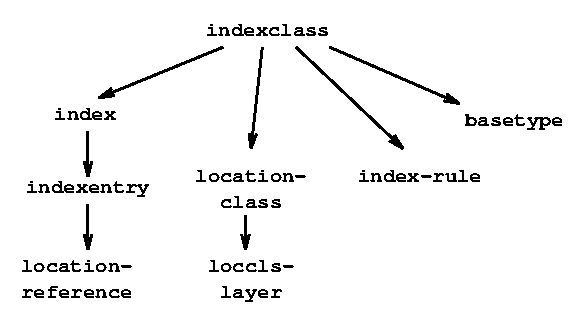
\epsfig{file=datenmodell.eps}
\end{tfigure}

In Abbildung~\ref{fig:vererbungsgraph} sind die wichtigsten
Vererbungsbeziehungen zwischen Klassen dargestellt. Sie sollen einen
�berblick �ber die dem System innewohnenden Beziehungen geben.
Weitere implementationsspezifische Vererbungsbeziehungen sind nicht
dargestellt. Der Modulgraph in Abbildung~\ref{fig:modulgraph} zeigt
die \emph{benutzt}-Relationen der Module.


\begin{tfigure}{Vererbungsgraphen der wichtigsten Klassen der Implementierung}
  {fig:vererbungsgraph}
  \centering
  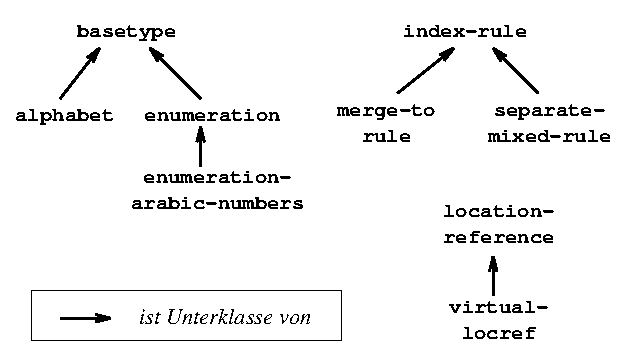
\epsfig{file=vererbungsgraph.eps}
\end{tfigure}

\begin{tfigure}{Modulgraph mit \emph{benutzt}-Relationen}
  {fig:modulgraph}
  \centering%%
  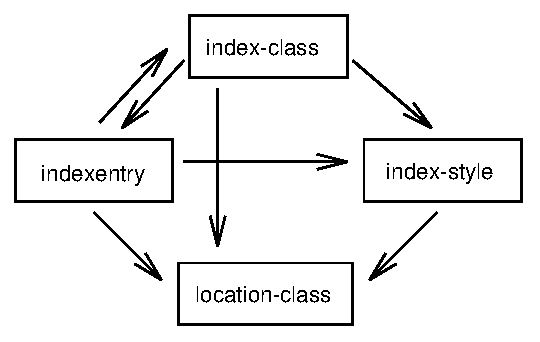
\epsfig{file=modulgraph.eps}
\end{tfigure}

%\afterpage{\clearpage}
\newpage

\section*{Klassenbeschreibungen}

Wir beschreiben nun f�r die angef�hrten Klassen ihre jeweilige
Funktion und die wichtigsten Komponenten und Methoden \bzw
Schnittstellen, um einen �berblick �ber das Gesamtsystem zu erhalten.

\begin{describeClass}{indexclass}
  Diese Klasse ist die oberste Datenstruktur im System. Sie enth�lt
  alle Definitionen, die zu einer Indexklasse geh�ren. Dazu geh�ren
  sowohl die Komponenten, die den Indexstyle definieren, als auch der
  Index selbst.
\end{describeClass}

\begin{describeComponents}
\item[name] Hier ist der Name der Indexklasse abgelegt. Es exisitiert
  immer eine Indexklasse mit Namen \texttt{default}.
\item[basetypes] Alle definierten Komponententypen werden hier
  abgelegt. Die Komponententypen werden �ber ihre Namen angesprochen.
  Die Elemente sind Instanzen der Klasse \texttt{basetype}.
\item[locclasses] Alle vom Benutzer definierten Lokationsklassen
  werden hier abgelegt. Die Elemente sind Instanzen der Klasse
  \texttt{location-class}.
\item[index] Hier ist der Index abgelegt. Es handelt sich um eine
  Instanz der \texttt{index}-Klasse.
\item[keyword-markup] Die Ausgabeformatierung f�r die Stichw�rter
  werden hier abgelegt.
\item[succ-table] ist die Tabelle mit den Nachfolgerdefinitionen.
  Hierin ist das \emph{Dokumentwissen} enthalten.
\item[merge-to-rules] sind die \textsf{merge-to}-Regeln. Sie sind
  Instanzen der Klasse \texttt{index-rule}.
\item[sep-mix-rule] enthalten die \textsf{separated-mixed}-Regeln.
\end{describeComponents}

\begin{describeMethods}
  Da die Klasse oberste Verwaltungseinheit ist, stehen im wesenlichen
  nur Operationen zum F�llen und Zugreifen der Komponenten zur
  Verf�gung.
\end{describeMethods}



\begin{describeClass}{basetype}
  Diese Klasse ist die abstrakte Basisklasse f�r Alphabete und
  Aufz�hlungen.
\end{describeClass}

\begin{describeComponents}
\item[name] enth�lt den Namen des Komponententyps.
\item[base-alphabet] das Basisalphabet des Komponententyps.
\end{describeComponents}

\begin{describeMethods}
  \begin{defgen}{prefix-match}{\farg{string} \farg{basetype}}
    Das Argument \farg{string} ist dieZeichenkette, \farg{basetype}
    ist eine Instanz eines Komponententyps. Die Funktion versucht,
    einen Pr�fix der Zeichenkette dem angegebenen Komponententyp
    zuzuordnen. Die Methoden m�ssen f�r alle abgeleiteten Klassen von
    \texttt{basetype} definiert sein und einen multiple-value der Form
    (\farg{matched-str} \farg{rest-str} \farg{ordnum}) zur�ckliefern.
    Dabei bezeichnet \farg{matched-str} eine Zeichenkette, die dem
    Komponententyp zugeordnet werden konnte, \farg{rest-str} der Rest
    der Zeichenkette und \farg{ordnum} die Ordnungszahl, die der
    Zeichenkette zugeordnet wurde.
  \end{defgen}
\end{describeMethods}



\begin{describeClass}{alphabet}
  Diese Klasse ist Basisklasse aller Alphabete und von
  \texttt{basetype} abgeleitet.
\end{describeClass}

\begin{describeComponents}
\item[symbols] enth�lt eine Liste aller Symbole des Alphabets. Ein
  Symbol ist dabei ein Wort �ber dem Basisalphabet. Wir ermitteln bei
  Alphabeten das Basisalphabet durch Analyse der Symbole des
  Alphabets.
\end{describeComponents}

\begin{describeMethods}
  Es ist eine allgemeine Methode \func{prefix-match} definiert, die
  das oben beschriebene Verhalten f�r alle Alphabete nachbildet.
\end{describeMethods}


%\newpage

\begin{describeClass}{enumeration}
  Diese Klasse ist Basisklasse aller Aufz�hlungen und von
  \texttt{basetype} abgeleitet.
\end{describeClass}

\begin{describeComponents}
\item[\normalfont\emph{Konstruktor}] Der Konstruktor bekommt das
  Basisalphabet �bergeben, da keine weiteren Informationen �ber die
  Aufz�hung bekannt sind.
\end{describeComponents}

\begin{describeMethods}
  Da Aufz�hlungen wie die arabischen oder die r�mischen Zahlen eine
  grund"-s�tz"-lich andere Struktur aufweisen als Alphabete, mu� f�r
  jede konkrete Aufz�hlung eine entsprechende Methode
  \func{prefix-match} implementiert werden.
\end{describeMethods}


\begin{describeClass}{location-class}
  Diese Klasse ist Container f�r alle zu einer Lokationsklasse
  geh�renden Informationen.
\end{describeClass}

\begin{describeComponents}
\item[name] enth�lt den Namen der Lokationsklasse.
\item[layers] enth"alt die Liste der Ebenen der Lokationsstruktur.
  Die Ebenen sind Instanzen der Klasse \texttt{loccls-layer}.
\item[join-layers] enth�lt eine Liste der Nummern aller
  Strukturkomponenten, die prinzipiell zur Bereichsbildung herangezogen
  werden d�rfen.
\item[ordnum] die einer Lokationsklasse zugeordnete Ordnungsnummer.
  Dies wird zur Definition eines Ordnungskriteriums auf
  Lokationsklassen f�r die Sortierung von Lokationsreferenzen
  ben�tigt. Das momentan implementierte Ordnungskriterium bezieht sich
  auf die Reihenfolge der Definitionen der Lokationsklassen.
  Lokationsreferenzen von fr�her definierten Lokationsklassen
  erscheinen bei der Ausgabe zuerst.
\end{describeComponents}

\begin{describeMethods}
  Die zugeordneten Methoden dienen dem Zugriff auf die Komponenten der
  Instanzen.
\end{describeMethods}


\begin{describeClass}{location-reference}
  Diese Klasse verwaltet eine Lokationsreferenz. Sie ist Container f�r
  die Strukturkomponenten und Attribute der Lokationsreferenz.
\end{describeClass}

\begin{describeComponents}
\item[layers] hierin finden sich die einzelnen Ebenen der
  Lokationsreferenz. Eine Ebene ist ein Objekt von Klasse
  \texttt{locref-layer}.
\item[ordnums] Die Ordnungszahlen der Ebenen werden hier abgelegt.
  Urspr�nglich wurde in jeder Ebene die zugeordnete Ordnungszahl
  abgelegt. Durch die Zusammenfassung in einer direkt zugreifbaren
  Liste wurde eine einfache Optimierung vorgenommen.
\item[optattr] beinhaltet den Namen des zugeordneten optischen Attributs.
\item[locclass] beinhaltet den Namen der zugeordneten Lokationsklasse.
\end{describeComponents}

\begin{describeMethods}
  \begin{defunc}{locref<}{\farg{locref-1} \farg{locref-2}}
    Diese Funktion vergleicht die Ordnungszahlen zweier
    Lokationsreferenzen und liefert \texttt{t} oder \texttt{nil}.
  \end{defunc}

  \begin{defmethod}{markup-object}{\farg{location-reference} \farg{markup}
      \farg{context} \farg{env-stack}}
    Implementiert die Ausgabeformatierung f�r eine Lokationsreferenz.
  \end{defmethod}
\end{describeMethods}



\begin{describeClass}{indexentry}
  Diese Klasse enth�lt alle Informationen �ber einen Indexeintrag. Sie
  stellt einen Container dar, der beim Einlesen eines Indexeintrags
  initialisiert wird.
\end{describeClass}

\begin{describeComponents}
\item[main-key] enth�lt den Hauptschl�ssel des Indexeintrags.
\item[merge-key] ist der Schl�ssel zum Mischen zweier Eintr�ge.
\item[sort-key] ist der Sortierschl�ssel.
\item[print-key] ist der Schl�ssel, der f�r die Ausgabe verwendet wird.
\item[locrefs] sind die dem Indexeintrag zugeordneten Lokationsreferenzen.
\end{describeComponents}

\begin{describeMethods}
  \begin{defunc}{process-indexentry}{\farg{indexentry}}
    Sortiert und mischt alle Lokationsreferenzen dieses Indexeintrags
    und bildet Bereiche aus aufeinanderfolgenden Referenzen.

    Diese Verarbeitung gliedert sich in verschiedene Unterprozesse.
    Die Funktionsweise folgt der in
    Abschnitt~\ref{sec:locrefmischung} beschriebenen Vorgehensweise.
    Die Lokationsreferenzen werden in Gruppen unterteilt, die zu
    verschiedenen Lokationsklassen geh�ren. Anschlie�end wird jede
    Gruppe gem�� der Regeln des separate- \bzw mixed-sorting
    unterteilt. Es folgt die Anwendung der \texttt{merge-to}-Regeln
    und eine Sortierung gem�� der Totalen Ordnung. Zuletzt werden die
    Bereiche gebildet.
  \end{defunc}

  \begin{defmethod}{markup-object}{\farg{indexentry} \farg{markup-list}
      \farg{context-list} \farg{env-stack}}
    Implementiert die Ausgabeformatierung f�r einen Indexeintrag.
  \end{defmethod}
\end{describeMethods}



\begin{describeClass}{index}
  Diese Klasse ist ein Container f�r die Liste der Indexeintr�ge.
\end{describeClass}

\begin{describeComponents}
\item[entries] enth�lt die Liste der Indexeintr�ge.
\end{describeComponents}

\begin{describeMethods}
  \begin{defunc}{indexentry=}{\farg{indexentry-1} \farg{indexentry-2}}
    �berpr�ft, ob zwei Indexeintr�ge bez�glich ihres Mischschl�ssels
    gleich sind.
  \end{defunc}

  \begin{defunc}{merge-indexentry-to-index}{\farg{indexentry} \farg{index}}
    F�gt einen Indexeintrag in den Index ein und vereinigt ihn
    gegebenenfalls mit einem Indexeintrag gleichen Mischschl�ssels.
  \end{defunc}

  \begin{defunc}{merge-indexentries}{\farg{indexentry-1} \farg{indexentry-2}}
    Vereinigt zwei Indexeintr�ge miteinander, deren Mischschl�ssel
    gleich sind und liefert einen neuen Indexeintrag (\emph{siehe
      Abschnitt~\ref{sec:stwmischung}}).
  \end{defunc}

  \begin{defmethod}{markup-object}{\farg{index} \farg{markup-list}
      \farg{context-list} \farg{env-stack}}
    Implementiert die Ausgabeformatierung f�r einen Index.
  \end{defmethod}

  \begin{defunc}{process-index}{\farg{indexclass}}
    Verarbeitet den zur Indexklasse \farg{indexclass} geh�renden Index.
  \end{defunc}
\end{describeMethods}



\begin{describeClass}{markup}
  Diese Klasse definiert die Markup-Struktur f�r die
  Ausgabeformatierung. Sie definiert Ausgabeprimitive f�r die
  \texttt{markup-object}-Methoden und behandelt die Verwaltung
  der ge�ffneten Umgebungen mittels eines Stacks.
\end{describeClass}

\begin{describeComponents}
\item[\ ] s�mtliche Komponenten wie in Abschnitt~\ref{sec:travAusgabebaum}
  beschrieben.
\end{describeComponents}

\begin{describeMethods}
  \begin{defgen}{markup-object}{\farg{index} \farg{markup}
      \farg{context} \farg{env-stack}}%
    Diese generische Funktion wird verwendet, um die Komponenten, die
    bei der Ausgabeformatierung beteiligt sind, mit einer
    einheitlichen Schnittstelle zu versehen.  Jede Komponente ben�tigt
    eine an die jeweilige Klasse gebundene Methode, f�gt ihre
    Ausgabekommandos in den Ausgabestrom hinzu und legt die
    Ausgabestrings f�r das Schlie�en von Formatierungsumgebungen auf
    den Environment-Stack.  Dieser Stack wird dann von der Funktion
    \texttt{close-environment} gegebenenfalls entleert.

    Wir beschreiben nun den Rumpf der
    \texttt{markup-object}-Methoden.  Die Punktnotation
    \emph{list}.\textsf{komp} liefert die Komponente \textsf{komp} des
    ersten Elements der Liste \emph{list}.
    \begin{algorithm}
      \FUNC \texttt{markup-object} (\F{object markup-list context-list
        env-stack})\\
      \BEGIN\\
        \>\F{object-list} := \flqq hole \F{object-list} aus
        \F{object}\frqq\\%%
        \>\WHILE \=(\F{context-list}.\textsf{value} ==
        \F{object-list}.\textsf{value}) \OR\\%%
        \>\>\>(\F{markup-list}.\textsf{typ} == \emph{aktiv})\\%%
        \>\>\F{counter}++\\%%
        \>\>\ACTION{\textsl{entferne erste Elemente aus}
          \F{object-list
          markup-list context-list}}\\%%
        \>\ENDWHILE\\%%
        \>\F{env-stack} := %%
        \F{close-environments}(\F{env-stack} \F{counter})\\%%
        \>\WHILE \NOT\ \F{empty}(\F{object-list})\\%%
        \>\>\F{mprint}(\F{markup-list}.\textsf{pre-node})\\%%
        \>\>\F{mprint}(\F{markup-list}.\textsf{pre-layer})\\%%
        \>\>\ACTION{drucke nun \F{object-list}.\textsf{value} \bzw
          \F{markup-list}.\textsf{repetition-symbol}}\\%%
        \>\>\F{mprint}(\F{markup-list}.\textsf{post-layer})\\%%

        \>\>\F{push}(\=$\{$\F{markup-list}.\textsf{post-node},
        \ACTION{\textsl{evtl. auch} \textsf{optional-post-layer}}$\}$,\\%%
          \>\>\>\F{env-stack})\\%%
          \>\>\ACTION{\textsl{entnehme erstes Element aus
              \F{object-list} und
            \F{markup-list}}}\\%%
        \>\ENDWHILE\\%%
        \>\ACTION{\textsl bearbeite Unterelemente von \F{object}}\\%%
        \ENDFUNC
    \end{algorithm}
  \end{defgen}


  \begin{defunc}{close-environments}{\farg{env-stack}\,
      \texttt{\&optional} \farg{stack-length}}%%
    Schlie�t die auf dem Stack ge�ffneten Umgebungen der
    Ausgabeformatierung bis der Stack nur noch die Tiefe
    \farg{stack-length} besitzt. Fehlt das optionale Argument so
    werden alle Umgebungen geschlossen. Der Stack wird in den
    \texttt{markup-object}-Methoden aufgebaut.
  \end{defunc}

  \begin{defgen}{mprint}{\farg{object}}
    Definiert eine generische Funktion f�r Ausgabeprimitive wie
    Strings und Zahlen. Entsprechende Methoden sind daf�r
    implementiert.
  \end{defgen}

\end{describeMethods}


%% Local Variables:
%% mode: latex
%% TeX-master: "makeindex4.tex"
%% End:

%%
%% $Log$
%% Revision 1.2  1995/10/20 11:57:34  kehr
%% Korrektur nach Klaus' Durchsicht.
%%
%% Revision 1.1  1995/10/16  17:31:52  kehr
%% Initial checkin of Report and Presentation.
%%
%% Revision 1.14  1995/10/06  23:05:14  kehr
%% Korrektur nach der Durchsicht von Karin.
%%
%% Revision 1.13  1995/09/22  01:12:03  kehr
%% Zweite �berarbeitung nch der inhaltlichen Korrektur. Au�erdem habe
%% ich das Logo zu MacIndex ver�ndert. Hat jetzt mehr pepp !
%%
%% Revision 1.12  1995/09/21  00:05:43  kehr
%% Erste Ver�nderungen nach der inhaltlichen Korrektur durch Joachim am
%% 20.Sep.95. Fast alle Dateien d'sind davon betroffen. Au�erdem sind noch zwei
%% neue Abbildungen hinzugekommen.
%%
%% Revision 1.11  1995/09/06  18:52:49  kehr
%% Made final changes before giving for correction.
%%
%% Revision 1.10  1995/08/28  18:08:14  kehr
%% Neue Einspielung der xfig-Dateien
%%
%% Revision 1.9  1995/07/04  09:46:29  kehr
%% Weitere �nderungen. Bin aber fast fertig.
%%
%% Revision 1.8  1995/07/04  00:46:51  kehr
%% Bald ist's soweit ;-)
%% Ich habe heute die generelle Umstrukturierung vorgenommen und einige
%% Teile herausgeschmissen. Die Indexverarbeitung mu� noch �berarbeitet werden.
%%
%% Revision 1.7  1995/06/18  19:10:37  kehr
%% Lokationsverarbeitung geblickt !;-)
%%
%% Revision 1.6  1995/06/17  20:36:29  kehr
%% Habe die Lokationsreferenzverarbeitung umstrukturiert und besser
%% definiert. DIe Buchstabengruppen m�ssen noch beendet werden und der
%% Algorithmus zum Mischen und Sortieren der Lokationsreferenzen mu�
%% fertiggestellt werden.
%%
%% Revision 1.5  1995/06/15  12:58:41  kehr
%% Erweiterung der Ausgabematrix und kleinere �nderungen am Layot.
%% �berpr�fe jetzt das ganze Dokument, um mich auf die beiden letzten
%% Probleme einzulesen.
%%
%% Revision 1.4  1995/06/13  21:55:15  kehr
%% Habe heute die Formulierung des Algorithmus controlled-jojo-traverse
%% fertiggestellt. Desweiteren Fehler in der Anwendung der \lindent-Umgebung
%% gefunden. Ich mu� noch die Matrix f�r die Definition der Ausgabekommandos
%% und der Angabe im Indexstyle entwickeln.
%%
%% Revision 1.3  1995/06/09  20:59:50  kehr
%% Superviel gemacht heute ;-)
%%
%% Revision 1.2  1995/06/08  20:19:47  kehr
%% Bibliographie erweitert.
%%
%% Revision 1.1  1995/06/08  11:25:58  kehr
%% Implementierungsteil angefangen.
%%
%%



%%
%% $Id$
%%
%% Document: Zusammenfassung des `makeindex4' - Projekts
%%



\chapter{Zusammenfassung}
\label{sec:zusammenfassung}

Das \mkxvier-System ist eine Weiterentwicklung der \textsf{makeindex}-
und \textit{International MakeIndex}-Systeme.
%%Dies soll durch die Namensgebung der Zahl vier im Index dargestellt
%%werden, da die Vorg�ngerversionen unter den Bezeichnungen 2.x und 3.x
%%verf�gbar sind.

Durch eine komplette theoretische Neuanalyse von Indexen konnten die
Erfordernisse an ein Indexsystem �berarbeitet werden. Die intensive
Analyse von Lokationsklassen und deren Verarbeitungsprozesse sowie die
neuartige universelle Ausgabeformatierung bilden den Hauptteil dieser
Studienarbeit.

%Daraus entstand nach einer datengerechten Modellierung das vorliegende
%System, welches auch dem Bedarf nach h�chstm�glicher
%Konfigurierbarkeit gerecht wird. Es stellt dem Benutzer ein
%leistungsf�higes Werkzeug zur Indexerstellung zur Verf�gung, dessen
%Grundstruktur m�glichst wenig Einschr�nkungen unterliegt.

Die Implementierungszeit konnte durch die vollst�ndige theoretische
Erarbeitung des Modells und der Verarbeitungsverfahren drastisch
verk�rzt werden.

W�hrend der Modellierung f�hrte vor allen Dingen die semantische
Bedeutung, die bestimmten Ausgabeformen von Lokationsreferenzen
zugeordnet werden mu�te, zu Problemen. Besondere Schwierigkeit lag in
der Kategorisierung von Ausgabeformen und inwieweit
Lokationsreferenzen unterdr�ckbar sein sollten. Wir haben uns hier zum
einen an existierende Indexe gehalten und zum anderen auch eigene
�berlegungen angestellt, die in die Modellierung eingeflossen sind.
Um die Komplexit�t niedrig zu halten und auch den Benutzer nicht mit
�bertriebener Konfigurierbarkeit zu �berfordern, haben wir uns
letztendlich f�r pragmatische, aber leistungsf�hige L�sungen
entschieden.

Die Erstellung eines Indexes ist generell auch eine Geschmacksfrage.
An dieser Stelle ist es aufgrund der Vielfalt der potentiellen W�nsche
der Autoren schwierig, eine zufriedenstellende Gesamtl�sung
auszuarbeiten.


\section*{Weiterf�hrende Arbeiten}
\label{sec:weiterArbeiten}

Im Rahmen der Modellierung eines Indexes und der damit verbundenen
Algorithmen sind zwei Probleme grunds�tzlicher Natur in den
Vordergrund getreten.

Das erste Problem ist die Erkenntnis, da� die Lokationsreferenzen als
Informationstr�ger �ber das zu indizierende Dokument nicht ausreichend
sind, um bestimmte in der Praxis vorkommende Indexe nachzubilden. Das
Hauptproblem ist in fehlendem Dokumentwissen\remark{Dokument\-wissen}
begr�ndet. Bereits die einfachste Gliederungsform in Punktnotation
(\textsf{1.2.3}\ldots) mit verschiedenen Gliederungstiefen macht die
Bestimmung des Nachfolgers einer Lokation unl�sbar, sofern dem System
die ben�tigten Informationen nicht zus"atzlich zugef�hrt werden.

Das zweite Problem besteht darin, da� ein Index sich auch
typographischen Satzregeln unterwerfen mu�, die \zB verlangen, da� die
Ersetzung von Stichw�rtern durch Wiederholungssymbole (\emph{siehe
  Abschnitt \ref{sec:travAusgabebaum}}) an Seiten- und
Spaltenanf�ngen unterdr�ckt werden sollte.\remark{textsatz\-abh�ngige
  Indexausgabe} Um dieses Problem zu l�sen, ben�tigt das
Textsatzsystem allerdings Informationen, die w�hrend des
Indexierungsvorgangs ermittelt werden.

Wie man sieht, sind diese Probleme nur dann l�sbar, wenn ein geeigneter
Informationsaustausch zwischen beiden Systemen stattfindet. Die
untersuchten Textsatzsysteme bieten allerdings keine direkte
Unterst�tzung, um ein Indexierungssystem direkt an den Textsatzproze�
anzukoppeln.

Interessant ist es die Spezifikation der Ausgabeformatierung und der
Regeln zum Sortieren und Mischen der Lokationsreferenzen zu
"uberarbeiten. Im Moment ist Wissen "uber die zugrundeliegenden
Algorithmen n"otig, um eine solche Spezifikation zu erstellen. Dies
ist jedoch f"ur einen Benutzer eine sehr unbefriedigende L"osung und
eine Untersuchung, ob \emph{interaktive} Werkzeuge dieses Problem
vereinfachen k"onnen, ist mit Sicherheit sinnvoll.

Des weiteren k�nnte es sinnvoll sein, das Konzept der Indexklassen
weiter zu untersuchen. Insbesondere k�nnte man sich mit der Bildung
einer Hierarchie von Klassen besch�ftigen, um Klasseneigenschaften
durch Vererbung\remark{Indexklassen\-vererbung} weiterzugeben. In
diesem Zusammenhang kann man auch die Gesamt- und Masterindexe und
ihre Eigenschaften vertieft untersuchen.


%% Local Variables:
%% mode: latex
%% TeX-master: "makeindex4.tex"
%% End:

%%
%% $Log$
%% Revision 1.2  1995/10/20 11:57:35  kehr
%% Korrektur nach Klaus' Durchsicht.
%%
%% Revision 1.1  1995/10/16  17:32:00  kehr
%% Initial checkin of Report and Presentation.
%%
%%



%%
%% $Id$
%%
%% Document: Glossar: `makeindex4' - Projekt
%%


\chapter{Glossar}
\label{sec:glossar}

\begin{tfigure}%
  {Index mit Bezeichnung der Komponenten eines Indexeintrags}%
  {fig:glo:1}%
  \centering
  \begin{minipage}{8cm}
    \begin{mkindex}
      \idx B�ume
      \subidx AVL, 3.3
      \subidx nat�rliche, 3.1
      \idx
      \fbox{%
        \fbox{Suche, bin�re}\,\footnote{Stichwort},%
        \fbox{%
          \fbox{2.2}\,\footnote{Strukturreferenz} %
          \fbox{\emph{f.}}\,\footnote{Lokationsattribut}%
          }\,\footnote{Attributierte Strukturreferenz}\,%
        }\,\footnote{Indexeintrag}
      \subidx sequentielle, 2.1
    \end{mkindex}
  \end{minipage}
\end{tfigure}


\begin{description}

\item[Attributierte Strukturreferenz] \mbox{}\\ Strukturreferenz, der
  ein zus�tzliches Attribut zugeordnet ist. Die Lokationsreferenz
  \quasi{35\emph{f.}}, die auf Seite 35 und die folgenden Seiten
  verweist, besteht aus der Strukturreferenz \Strukeins{35} und dem
  Attribut \quasi{\emph{f.}}.

\item[Basisalphabet] \mbox{}\\ Teilmenge eines Dokumentalphabets.
  \emph{Siehe auch Definition~\ref{def:basisalphabet},
    S.\,\pageref{def:basisalphabet}}.


\item[Dokumentalphabet] \mbox{}\\ Gemeinsames zugrundeliegendes
  Alphabet des Textsatzsystems und des Indexsystems. �blicherweise
  ASCII, ISO-Latin--Familie oder Unicode. \emph{Siehe auch
    Definition~\ref{def:dokumentalphabet},
    S.\,\pageref{def:dokumentalphabet}}.

\item[Dokumentwissen] \mbox{}\\ Bezeichnet Informationen, die in der
  Struktur des Dokumentes abgelegt sind und dem Indexierungssystem zur
  korrekten Bildung von Lokationsbereichen mitgeteilt werden m�ssen.
  \emph{Siehe Abschnitt~\ref{sec:nachfolger}}.

\item[Hierarchieebene] \mbox{}\\ Bezeichnet eine einzelne Ebene eines
  hierarchisch untergliederten Stichworts. Das Stichwort
  \Hierzwei{Suche}{bin�re} besteht aus den Hierarchieebenen
  \quasi{Suche} und \quasi{bin�re}.

\item[Index] \mbox{}\\ Bezeichnet ein Stichwortverzeichnis im �blichen
  Sinne. Es besteht aus einer Liste von sortierten Indexeintr�gen.

\item[Indexeintrag] \mbox{}\\ Besteht aus einem Stichwort und einer
  Menge von Lokationsreferenzen. \emph{Siehe auch
    Abbildung~\ref{fig:glo:1}}.

\item[Kategorieattribut] \mbox{}\\ Lokationsreferenzattribut, welches
  zu Kategorisierungszwecken verwendet wird und vom Textsatzsystem zur
  unterschiedlichen optischen Hervorhebung von Lokationsreferenzen
  verwendet werden kann. \emph{Siehe auch
    Abschnitt~\ref{sec:kategorieattribute}}.

\item[Komponententyp] \mbox{}\\ Bezeichnet den Typ einer
  Strukturkomponente.

\item[Lokation] \mbox{}\\ Strukturelles Objekt \bzw Element eines
  Textes. Beispiele f�r solche Lokationen sind \emph{Seiten},
  \emph{Kapitel}, \emph{Abschnitte}, \emph{Unterabschnitte},
  \emph{Anh�nge} \etc{}\,. Jede Lokation kann in einem Dokument nur
  ein einziges Mal auftreten und mu� eindeutig auf"|findbar sein.

\item[Lokationsreferenz] \mbox{}\\ Eindeutiger Bezeichner, der einer
  Lokation zugeordnet ist. Die Lokationsreferenz \quasi{Seite 51}
  verweist auf eindeutige Weise auf bestimmtes Objekt des Dokuments,
  eben die 51.\ Seite.

  %Im \mkxvier{}--System wird eine Lokationsreferenz als
  %\emph{Attributierte Strukturreferenz} behandelt.

\item[Permutierter Index] \mbox{}\\ Enh�lt zu jedem hierarchisch
  gegliederten Stichwort wie \Hierzwei{Suche}{bin�re} auch
  Permutationen der Stichworthierarchien wie \zB
  \Hierzwei{bin�re}{Suche}. \emph{Siehe dazu auch
    Abschnitt~\ref{index:permutierter}}\,.

\item[Referenz] ist gleichbedeutend mit \emph{Lokationsreferenz}.

\item[Sortieralphabet] \mbox{}\\ Definiert ein Alphabet von Worten
  �ber einem Basisalphabet. Ein solches Alphabet bestimmt die
  Sortierordnung innerhalb von Strukturkomponenten einer Lokationsreferenz.
  \emph{Siehe auch Definition~\ref{def:sortierungsalphabet},
    S.\,\pageref{def:sortierungsalphabet}}.

\item[Stichwort] \mbox{}\\ Begriff, auf dessen Vorkommen innerhalb
  eines Textes verwiesen werden soll. Ein strukturierter
  Begriff kann sich aus mehreren Ebenen zusammensetzen. Im
  Beispiel~\ref{fig:glo:1} haben wir die Stichw�rter
  \Hierzwei{B�ume}{AVL}, \Hierzwei{B�ume}{nat�rliche} und
  \Hierzwei{Suche}{bin�re}. Wir verstehen hier als Stichwort alle
  zusammengeh�renden Ebenen eines Begriffs.

\item[Strukturkomponente] \mbox{}\\ Teilkomponente der Struktur einer
  Lokationsreferenz. Die Lokationsreferenz \Strukdrei{3}{.}{1}{.}{2}
  besteht aus den Strukturkomponenten \Strukebene{3}, \Strukebene{1} und
  \Strukebene{2}.

\item[Strukturreferenz] \mbox{}\\ Beschreibt die strukturelle
  Zusammensetzung einer Lokationsreferenz. Die Struktur einer Referenz
  ergibt sich aus der Folge der Strukturkomponenten und der Trennzeichen
  zwischen den Ebenen. Die Lokation \mbox{\quasi{Kapitel--1}} besteht
  aus der 1.\ Ebene \quasi{Kapitel}, dem Trennzeichen \quasi{--} und
  der 2.\ Ebene \quasi{1}. Wir notieren solche Strukturreferenzen als
  \Strukzwei{Kapitel}{--}{1}. Weitere Beispiele sind der Abschnitt
  \Strukdrei{1}{.}{2}{.}{3} oder die Seite \Strukeins{23}.

\end{description}


%% Local Variables:
%% mode: latex
%% TeX-master: "makeindex4.tex"
%% End:

%%
%% $Log$
%% Revision 1.1  1995/10/16 17:31:51  kehr
%% Initial checkin of Report and Presentation.
%%
%% Revision 1.13  1995/10/06  23:05:13  kehr
%% Korrektur nach der Durchsicht von Karin.
%%
%% Revision 1.12  1995/09/22  01:12:02  kehr
%% Zweite �berarbeitung nch der inhaltlichen Korrektur. Au�erdem habe
%% ich das Logo zu MacIndex ver�ndert. Hat jetzt mehr pepp !
%%
%% Revision 1.11  1995/09/21  00:05:42  kehr
%% Erste Ver�nderungen nach der inhaltlichen Korrektur durch Joachim am
%% 20.Sep.95. Fast alle Dateien d'sind davon betroffen. Au�erdem sind noch zwei
%% neue Abbildungen hinzugekommen.
%%
%% Revision 1.10  1995/08/28  18:08:13  kehr
%% Neue Einspielung der xfig-Dateien
%%
%% Revision 1.9  1995/07/04  00:46:50  kehr
%% Bald ist's soweit ;-)
%% Ich habe heute die generelle Umstrukturierung vorgenommen und einige
%% Teile herausgeschmissen. Die Indexverarbeitung mu� noch �berarbeitet werden.
%%
%% Revision 1.8  1995/06/17  20:36:29  kehr
%% Habe die Lokationsreferenzverarbeitung umstrukturiert und besser
%% definiert. DIe Buchstabengruppen m�ssen noch beendet werden und der
%% Algorithmus zum Mischen und Sortieren der Lokationsreferenzen mu�
%% fertiggestellt werden.
%%
%% Revision 1.7  1995/06/09  20:59:49  kehr
%% Superviel gemacht heute ;-)
%%
%% Revision 1.6  1995/06/08  20:19:47  kehr
%% Bibliographie erweitert.
%%
%% Revision 1.5  1995/06/07  20:59:12  kehr
%% Und weiter am Modellentwurf. Spezifikation des Indexstyles vorerst
%% fertig. Es fehlt noch die Eingabegrammatik.
%%
%% Revision 1.4  1995/05/31  19:18:51  kehr
%% Fertigstellung des Analyse-Abschnitts (Hoffentlich ;-).
%%
%% Revision 1.3  1995/05/31  16:14:57  kehr
%% Dokumant- und Sortierungsalphabet entwickelt. Makefile�nderungen und
%% Stylever�nderungen.
%%
%% Revision 1.2  1995/05/29  00:22:43  kehr
%% Die Einleitung ist somweit fertig und die Analyse mu� jetzt noch
%% beendet werden. Mir fehlt da noch eine vern�nftige Idde f�r die
%% Alphabete und deren Definitionen.
%%
% Revision 1.1  1995/05/28  21:37:10  kehr
% Neue �berarbeitete Version.
% Inhaltliche �nderungen:
%   Glossar hinzugenommen. Einleitung mit Datenflu�graph. Kleinere
%   �nderungen an der Beschreibung des International Makeindex.
% System�nderungen:
%   Makefile-�nderungen, Stil�nderungen, Titelseite
%
%%



\bibliography{bibliographie}
%%\bibliographystyle{apalike}
\bibliographystyle{alpha}

%%
%% $Id$
%%
%% Document: 
%%
%%

\end{document}



%% Local Variables:
%% mode: latex
%% TeX-command-default: "LaTeX"
%% TeX-master: t
%% End:

%%
%% $Log$
%% Revision 1.1  1995/10/16 17:31:59  kehr
%% Initial checkin of Report and Presentation.
%%
%% Revision 1.13  1995/10/06  23:05:15  kehr
%% Korrektur nach der Durchsicht von Karin.
%%
%% Revision 1.12  1995/09/06  18:52:50  kehr
%% Made final changes before giving for correction.
%%
%% Revision 1.11  1995/08/28  18:08:15  kehr
%% Neue Einspielung der xfig-Dateien
%%
%% Revision 1.10  1995/06/08  11:25:58  kehr
%% Implementierungsteil angefangen.
%%
%% Revision 1.9  1995/06/06  17:51:02  kehr
%% Commit um die �nderungen festzuhalten.
%%
%% Revision 1.8  1995/05/31  19:18:52  kehr
%% Fertigstellung des Analyse-Abschnitts (Hoffentlich ;-).
%%
%% Revision 1.7  1995/05/31  16:14:58  kehr
%% Dokumant- und Sortierungsalphabet entwickelt. Makefile�nderungen und
%% Stylever�nderungen.
%%
%% Revision 1.6  1995/05/29  00:22:43  kehr
%% Die Einleitung ist somweit fertig und die Analyse mu� jetzt noch
%% beendet werden. Mir fehlt da noch eine vern�nftige Idde f�r die
%% Alphabete und deren Definitionen.
%%
%% Revision 1.5  1995/05/28  21:37:10  kehr
%% Neue �berarbeitete Version.
%% Inhaltliche �nderungen:
%%   Glossar hinzugenommen. Einleitung mit Datenflu�graph. Kleinere
%%   �nderungen an der Beschreibung des International Makeindex.
%% System�nderungen:
%%   Makefile-�nderungen, Stil�nderungen, Titelseite
%%
%% Revision 1.4  1995/05/05  22:25:03  kehr
%% Ge�nderte Struktur mit einleitung.tex
%% Zwischenspeicherung vor der Umstellung der Definitionen
%%
%% Revision 1.3  1995/04/30  16:14:10  kehr
%% Trennung in Einleitung, Einf�hrung und Analyse. Evtl. sollten die Filenamen
%% entsprechend anepa�t werden. Dar�berhinaus Analyse weitergef�hrt.
%%
%% Revision 1.2  1995/04/25  01:09:39  kehr
%% Analyse und Modellentwurf weitergebracht.
%%
%% Revision 1.1  1995/04/22  21:05:41  kehr
%% Erstes Setup der Studienarbeit des Makeindex4-Projektes
%%
